\documentclass[handout]{beamer}
\usepackage{templates/beamerthemekitwide}

\usepackage[utf8]{inputenc}
\usepackage[T1]{fontenc}
\usepackage[ngerman]{babel}
\usepackage{listings}
\usepackage{hyperref}
\usepackage{graphicx}

\usepackage{amsmath}
\usepackage{amsthm}
\usepackage{amssymb}
\usepackage{polynom}

%\usepackage{ifthen}
%\usepackage{adjustbox} % for \adjincludegraphics

%\usepackage{tikz}
\usepackage{listings}

%\usepackage[]{algorithm2e}

%\usepackage{colortbl}
\usepackage{verbatim}
%\usepackage{alltt}
%\usepackage{changes}

%\usepackage{pdfpages}
%\usepackage{tabularx}

%\usepackage{euler}


\newcommand{\markBlue}[1]{\textcolor{kit-blue100}{#1}}
\newcommand{\markGreen}[1]{\textcolor{kit-green100}{#1}}
\newcommand{\vertspace}{\vspace{.2cm}}

%\newcommand{\#}{\markBlue{#1}}

%\newcommand{\pitem}{\pause\item}
\newcommand{\p}{\pause}

% -- MATH MACROS
\newcommand{\thistheoremname}{}
\newcommand{\G}{\mathbb{Z}}
\newcommand{\B}{\mathbb{B}}
\newcommand{\R}{\mathbb{R}}
\newcommand{\N}{\mathbb{N}}
\newcommand{\Q}{\mathbb{Q}}
\newcommand{\C}{\mathbb{C}}
\newcommand{\Z}{\mathbb{Z}}
\newcommand{\F}{\mathbb{F}}
\newcommand{\mi}{\mathrm{i}}
\renewcommand{\epsilon}{\varepsilon}
\newcommand{\okalk}{\mathscr{O}}


\newenvironment<>{taskblock}[1]{%
	\setbeamercolor{block title}{fg=kit-orange15,bg=kit-orange100}
	\setbeamercolor{block body}{fg=black,bg=kit-orange30}%
	\begin{block}#2{#1}}{\end{block}}

\setbeamertemplate{enumerate items}[default]

% Aussagenlogik Symbole
\newcommand{\W}{w}
\renewcommand{\F}{f}

% Kodierung
\newcommand{\frepr}{\textbf{repr}}
\newcommand{\fRepr}{\textbf{Repr}}
\newcommand{\fZkpl}{\textbf{Zkpl}}
\newcommand{\fbin}{\textbf{bin}}
\newcommand{\fdiv}{\textbf{ div }}
\newcommand{\fmod}{\textbf{ mod }}

% Speicherabbild
\newenvironment{memory}{\begin{tabular}{r | l}Adresse&Wert\\\hline\hline}{\end{tabular}}
\newcommand{\memrow}[2]{#1 & #2 \\\hline}

% Praedikatenlogik
\newcommand{\objequiv}{\stackrel{\cdot}{=}}
\newcommand{\pval}{val_{D,I,\beta}}

% Neue Befehle
\newcommand{\ip}{\pause} % inline pause, für mitten im satz
\newcommand{\pitem}{\pause\item} % für aufzählungen
\newcommand{\bp}{\pause} % block pause, für zwischen blöcken

\title[Grundbegriffe der Informatik]{Grundbegriffe der Informatik\\Tutorium 33}
\subtitle{}
\author{Lukas Bach, lukas.bach@student.kit.edu}
\date{gbi.lukasbach.com}

\institute{Tutorium im Wintersemester 2016/2017}

\titlelogo{lukasbach}

\titleimage{bg}

\setbeamercovered{invisible}

\renewcommand{\subsection}[1]{}
\renewcommand{\section}[1]{\begin{frame}\vfill\centering \huge\markBlue{#1} \vfill\end{frame}}

\begin{document}
	
	\selectlanguage{ngerman}
	
	%title page
	\begin{frame}
		\titlepage
	\end{frame}
	
	
\def\compiletype{print}

%\ifdefined\compileall

\begin{frame}\vfill\centering \huge\markGreen{Tutorium vom \tutdate} \vfill\end{frame}

\else
\ifdefined\compiletype
	\documentclass[handout]{beamer}
\else
	\documentclass{beamer}
	\def\compiletype{livebeamer}
\fi

\usepackage{templates/beamerthemekitwide}
%\usepackage{enumitem}

\usepackage[utf8]{inputenc}
\usepackage[T1]{fontenc}
\usepackage[ngerman]{babel}
\usepackage{listings}
\usepackage{hyperref}
\usepackage{graphicx}

\usepackage{amsmath}
\usepackage{amsthm}
\usepackage{amssymb}
\usepackage{polynom}

%\usepackage{ifthen}
%\usepackage{adjustbox} % for \adjincludegraphics

%\usepackage{tikz}
\usepackage{listings}

%\usepackage[]{algorithm2e}

%\usepackage{colortbl}
\usepackage{verbatim}
%\usepackage{alltt}
%\usepackage{changes}

%\usepackage{pdfpages}
%\usepackage{tabularx}

%\usepackage{euler}


\newcommand{\markBlue}[1]{\textcolor{kit-blue100}{#1}}
\newcommand{\markGreen}[1]{\textcolor{kit-green100}{#1}}
\newcommand{\vertspace}{\vspace{.2cm}}

%\newcommand{\#}{\markBlue{#1}}

%\newcommand{\pitem}{\pause\item}
\newcommand{\p}{\pause}

% -- MATH MACROS
\newcommand{\thistheoremname}{}
\newcommand{\G}{\mathbb{Z}}
\newcommand{\B}{\mathbb{B}}
\newcommand{\R}{\mathbb{R}}
\newcommand{\N}{\mathbb{N}}
\newcommand{\Q}{\mathbb{Q}}
\newcommand{\C}{\mathbb{C}}
\newcommand{\Z}{\mathbb{Z}}
\newcommand{\F}{\mathbb{F}}
\newcommand{\mi}{\mathrm{i}}
\renewcommand{\epsilon}{\varepsilon}
\newcommand{\okalk}{\mathscr{O}}


\newenvironment<>{taskblock}[1]{%
	\setbeamercolor{block title}{fg=kit-orange15,bg=kit-orange100}
	\setbeamercolor{block body}{fg=black,bg=kit-orange30}%
	\begin{block}#2{#1}}{\end{block}}

\setbeamertemplate{enumerate items}[default]

% Aussagenlogik Symbole
\newcommand{\W}{w}
\renewcommand{\F}{f}

% Kodierung
\newcommand{\frepr}{\textbf{repr}}
\newcommand{\fRepr}{\textbf{Repr}}
\newcommand{\fZkpl}{\textbf{Zkpl}}
\newcommand{\fbin}{\textbf{bin}}
\newcommand{\fdiv}{\textbf{ div }}
\newcommand{\fmod}{\textbf{ mod }}

% Speicherabbild
\newenvironment{memory}{\begin{tabular}{r | l}Adresse&Wert\\\hline\hline}{\end{tabular}}
\newcommand{\memrow}[2]{#1 & #2 \\\hline}

% Praedikatenlogik
\newcommand{\objequiv}{\stackrel{\cdot}{=}}
\newcommand{\pval}{val_{D,I,\beta}}

% Neue Befehle
\newcommand{\ip}{\pause} % inline pause, für mitten im satz
\newcommand{\pitem}{\pause\item} % für aufzählungen
\newcommand{\bp}{\pause} % block pause, für zwischen blöcken

\title[Grundbegriffe der Informatik]{Grundbegriffe der Informatik\\Tutorium 36}
\date{\tutdate}
\subtitle{}
\author{Maximilian Staab, \texttt{uxhdf@student.kit.edu}}



\institute{}

%\titlelogo{lukasbach}

\titleimage{bg}
%\titleimage{bg-advent}


\ifthenelse{\equal{\compiletype}{livebeamer}}
	{
		\def\livebeamermode{1}
	}{}

\ifthenelse{\equal{\compiletype}{print}}
	{
		\def\printmode{1}
	}{}

\setbeamercovered{invisible}

%\usepackage[citestyle=authoryear,bibstyle=numeric,hyperref,backend=biber]{biblatex}
%\addbibresource{templates/example.bib}
%\bibhang1em

\begin{document}
	
\selectlanguage{ngerman}


%title page
\begin{frame}
	\titlepage
\end{frame}

%table of contents
\ifdefined\printmode
	\ifdefined\compileall \else
	\begin{frame}{Gliederung}
		\tableofcontents
	\end{frame}
\fi\fi

\fi

\def\compileall{1}

\def\tutdate{08.02.2018}

\documentclass{beamer}
\usepackage{../templates/beamerthemekit}
%\usepackage{enumitem}

\usepackage[utf8]{inputenc}
\usepackage[T1]{fontenc}
\usepackage[ngerman]{babel}
\usepackage{listings}
\usepackage{hyperref}
\usepackage{graphicx}

\usepackage{amsmath}
\usepackage{amsthm}
\usepackage{amssymb}
\usepackage{polynom}

%\usepackage{ifthen}
%\usepackage{adjustbox} % for \adjincludegraphics

%\usepackage{tikz}
\usepackage{listings}

%\usepackage[]{algorithm2e}

%\usepackage{colortbl}
\usepackage{verbatim}
%\usepackage{alltt}
%\usepackage{changes}

%\usepackage{pdfpages}
%\usepackage{tabularx}

%\usepackage{euler}


\newcommand{\markBlue}[1]{\textcolor{kit-blue100}{#1}}
\newcommand{\markGreen}[1]{\textcolor{kit-green100}{#1}}
\newcommand{\vertspace}{\vspace{.2cm}}

%\newcommand{\#}{\markBlue{#1}}

%\newcommand{\pitem}{\pause\item}
\newcommand{\p}{\pause}

% -- MATH MACROS
\newcommand{\thistheoremname}{}
\newcommand{\G}{\mathbb{Z}}
\newcommand{\B}{\mathbb{B}}
\newcommand{\R}{\mathbb{R}}
\newcommand{\N}{\mathbb{N}}
\newcommand{\Q}{\mathbb{Q}}
\newcommand{\C}{\mathbb{C}}
\newcommand{\Z}{\mathbb{Z}}
\newcommand{\F}{\mathbb{F}}
\newcommand{\mi}{\mathrm{i}}
\renewcommand{\epsilon}{\varepsilon}
\newcommand{\okalk}{\mathscr{O}}


\newenvironment<>{taskblock}[1]{%
	\setbeamercolor{block title}{fg=kit-orange15,bg=kit-orange100}
	\setbeamercolor{block body}{fg=black,bg=kit-orange30}%
	\begin{block}#2{#1}}{\end{block}}

\setbeamertemplate{enumerate items}[default]

% Aussagenlogik Symbole
\newcommand{\W}{w}
\renewcommand{\F}{f}

% Kodierung
\newcommand{\frepr}{\textbf{repr}}
\newcommand{\fRepr}{\textbf{Repr}}
\newcommand{\fZkpl}{\textbf{Zkpl}}
\newcommand{\fbin}{\textbf{bin}}
\newcommand{\fdiv}{\textbf{ div }}
\newcommand{\fmod}{\textbf{ mod }}

% Speicherabbild
\newenvironment{memory}{\begin{tabular}{r | l}Adresse&Wert\\\hline\hline}{\end{tabular}}
\newcommand{\memrow}[2]{#1 & #2 \\\hline}

% Praedikatenlogik
\newcommand{\objequiv}{\stackrel{\cdot}{=}}
\newcommand{\pval}{val_{D,I,\beta}}

% Neue Befehle
\newcommand{\ip}{\pause} % inline pause, für mitten im satz
\newcommand{\pitem}{\pause\item} % für aufzählungen
\newcommand{\bp}{\pause} % block pause, für zwischen blöcken
\title[Grundbegriffe der Informatik]{ICPC\\Gruppe 2}
\date{\tutdate}
\subtitle{\tutTitle}
\author{Elias Schaut, Dennis Kobert, Niklas Kniep, Lam Vo, Ilia Bozhinov}

\institute{}

\titleimage{bg}
%\titleimage{bg-advent}

%
\ifthenelse{\equal{\compiletype}{livebeamer}}
	{
		\def\livebeamermode{1}
	}{}

\ifthenelse{\equal{\compiletype}{print}}
	{
		\def\printmode{1}
	}{}

\setbeamercovered{invisible}

%\usepackage[citestyle=authoryear,bibstyle=numeric,hyperref,backend=biber]{biblatex}
%\addbibresource{templates/example.bib}
%\bibhang1em

	
\def\tutTitle{Turingmaschinen, Reguläre Sprachen}
\begin{document}

\selectlanguage{ngerman}

%title page
\begin{frame}
	\titlepage
\end{frame}

\section{Turingmaschinen}


\begin{frame}{Definition von Turingmaschinen}
	\begin{block}{Definition von Turingmaschinen}
		Eine Turingmaschine $T = (Z, z_0, X, f, g, m)$ besteht aus:
		\begin{itemize}
			\item $Z$ Zustandsmenge
			\item $z_0 \in Z$ Startzustand
			\item $X$ Bandalphabet
			\item $\Box$ Blanksymbol (sozusagen Markierung für Leerzeichen)
			\item $f: Z \times X \rightarrow Z$ partielle Zustandsübergangsfunktion
			\item $g: Z \times X \rightarrow X$ partielle Ausgabefunktion
			\item $m: Z \times X \rightarrow \{L, N, R\}$ partielle Bewegungsfunktion
		\end{itemize}
	\end{block}

	Anmerkung: partielle Funktionen sind \markGreen{nicht linkstotal}, also manche Elemente des Definitionsbereichs werden nicht abgebildet.
\end{frame}

\begin{frame}{Beispiel einer Turingmaschine}
	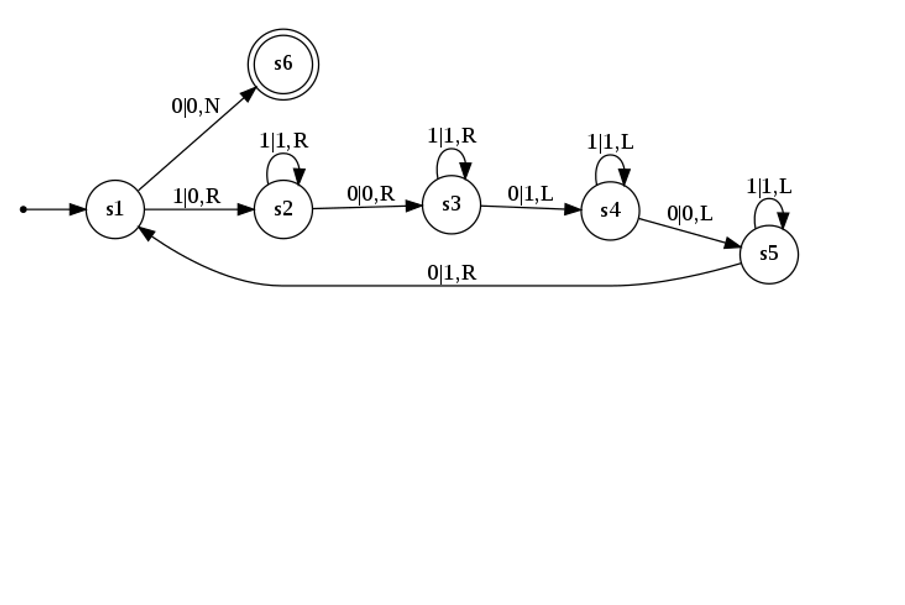
\includegraphics[scale=0.5]{images/turingexample_withoutannotations.png}
\end{frame}

\begin{frame}{Halten von Turingmaschinen}
	
	\p
	
	\begin{block}{Halten einer Turingmaschine}
		Wenn eine Turingmaschine in einem Zustand ist, für den das nächste Eingabezeichen durch die Übergangsfunktion $f$ nicht definiert ist, \markGreen{hält} die Maschine.
	\end{block}

	\bp

	Wann hält also eine Turingmaschine \markBlue{nicht}?
	
	\bp
	
	\begin{block}{Nicht-Halten einer Turingmmaschine}
		Wenn eine Turingmaschine in eine endlose Schleife gerät, so \markGreen{hält sie nicht}.
	\end{block}
\end{frame}

\begin{frame}{Entscheidbarkeit}
	\ip
	
	\begin{block}{Durch Turingmaschine akzeptierte Sprache}
		Eine Turingmaschine \markBlue{akzeptiert} eine formale Sprache $L$, wenn sie für jedes Wort $w \in L$ in einem akzeptierenden Zustand hält.
	\end{block}

	\bp

	\begin{block}{Entscheidbare Sprache}
		Eine formale Sprache $L$ heißt \markBlue{entscheidbar}, wenn es eine Turingmaschine gibt, die \markGreen{immer hält} und $L$ akzeptiert.
	\end{block}

	\bp

	\begin{block}{Aufzählbare Sprache}
		Eine formale Sprache $L$ heißt \markBlue{aufzählbar}, wenn es eine Turingmaschine gibt, die $L$ akzeptiert.
	\end{block}
\end{frame}

\begin{frame}{Vom endlichen Akzeptor zur Turingmaschine}
	\begin{taskblock}{Akzeptieren von Turingmaschinen}
		Wie kann man aus dem gegebenen endlichen Akzeptor eine Turingmaschine machen, die dieselbe Sprache akzeptiert?
	\end{taskblock}

	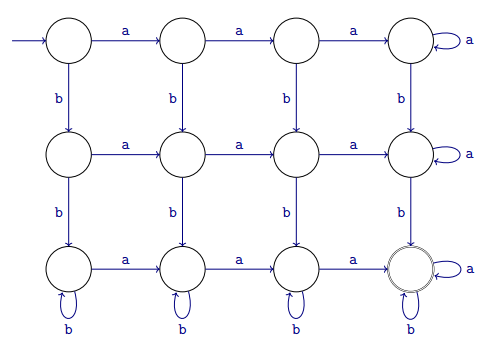
\includegraphics[scale=0.5]{images/AufgAkzeptor2.png}
\end{frame}

\begin{frame}{Lösung}
	Einfach gesagt: mache aus jedem Übergang $a$ einen Turingmaschinen-Übergang der Art $a|a,R$, also bei jedem Zeichen mache den Zustandsübergang, überschreibe aber das Zeichen nicht und gehe zum nächsten Zeichen.
	
	\vspace{.2cm}
	\bp
	
	Formaler ausgedrückt? \pause 
	\begin{itemize}
		\item Für allgemeinen endlichen Akzeptor $(Z, z_0, X, f, Y, h)$, definiere eine Turingmaschine $T := (Z, z_0, X \cup Y, f, g, h)$, also $Z, z_0, f$ gleich und mit Bandalphabet $=$ Eingabealphabet $\cup$ Ausgabealphabet
		\item $g(z, x) := x \quad \forall (z,x)$ in $f$ definiert
		\item $m(z, x) := R \quad \forall (z,y)$ in $f$ definiert		
	\end{itemize}

	\bp
	
	Jeder endliche Akzeptor kann so zu einer Turingmaschine umgeformt werden, die dieselbe Sprache akzeptiert.
\end{frame}

\begin{frame}{Über endliche Akzeptoren hinaus}
	Sei $L$ die Sprache von Palindromen über $\{a,b\}$ ($L = \{aabaa, bbababb, aa, \epsilon\}$). 
	
	\begin{itemize}
		\pitem Ist die Sprache regulär, also gibt es einen endlichen Akzeptor, der diese akzeptiert? \pause Nein.
		\pitem Ist die Sprache entscheidbar, also gibt es eine stets haltende Turingmaschine, die $L$ akzeptiert?
	\end{itemize}
\end{frame}

\begin{frame}{Palindromerkennung mit Turingmaschinen}
	Ja, nämlich: 
		
	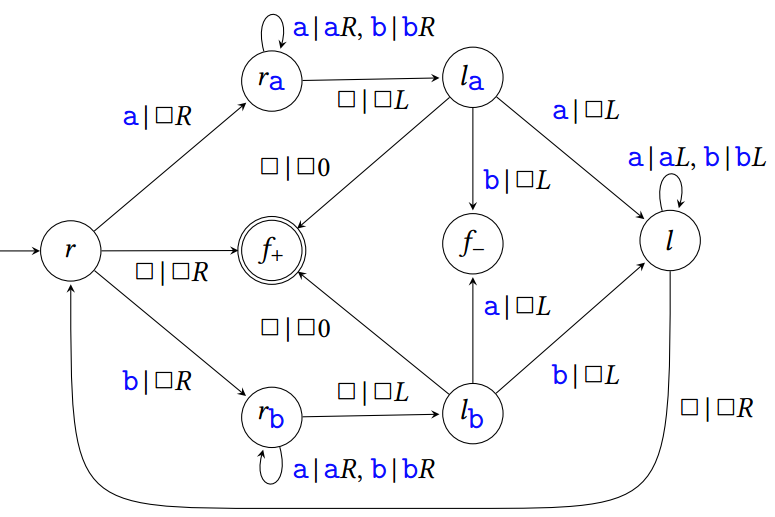
\includegraphics[scale=0.4]{images/turingmaschine_palindrome.png}	
\end{frame}

\begin{frame}{Turingmaschinen Entwurfsaufgabe}
	
	\begin{columns}
		\begin{column}{0.65\textwidth}
			\begin{taskblock}{Turingmaschine Entwurf}
				Entwerfe eine Turingmaschine, die...
				\begin{itemize}
					\item als Eingabe eine Binärzahl auf dem Band erhält
					\item als Ausgabe diese Zahl restlos durch zwei teilt und auf dem Band stehen lässt
				\end{itemize}
			\end{taskblock}
		\end{column}
		
		\begin{column}{0.45\textwidth}
			\pause
			
			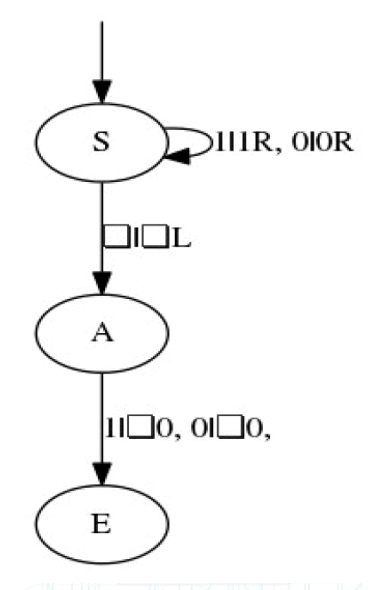
\includegraphics[scale=0.5]{images/turingmaschine_div.png}
		\end{column}
	\end{columns}

\end{frame}

\begin{frame}{Turingmaschinen Entwurfsaufgabe}
	
	\begin{columns}
		\begin{column}{0.65\textwidth}
			\begin{taskblock}{Turingmaschine Entwurf}
				Entwerfe eine Turingmaschine, die...
				\begin{itemize}
					\item als Eingabe eine Binärzahl auf dem Band erhält
					\item als Ausgabe diese Zahl um eins erhöht auf dem Band stehen lässt
					\item den Kopf der Turingmaschine auf dem ersten Zeichen der Ausgabe stehen hat.
				\end{itemize}
			\end{taskblock}
		\end{column}
		
		\begin{column}{0.45\textwidth}
			\pause
			
			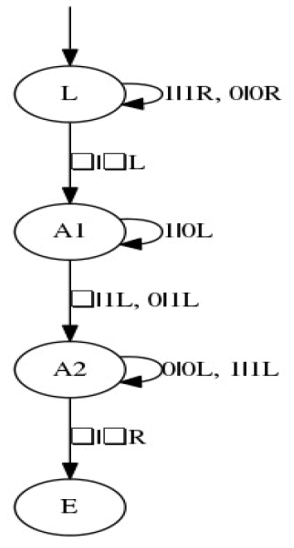
\includegraphics[scale=0.5]{images/turingmaschine_plusone.png}
		\end{column}
	\end{columns}
	
\end{frame}

\begin{frame}{Konfiguration von Turingmaschinen}
	Angenommen, man kennt eine Turingmaschine, hat mit der Abarbeitung eines Wortes angefangen, will aber pausieren, um später weiterzumachen...
	
	\vspace{.2cm}
	
	Was muss man sich alles merken, um später weiter zu machen?
	
	\begin{itemize}
		\pitem Derzeitiger Zustand, in dem die Turingmaschine steht
		\pitem Inhalt des Bandes
	\end{itemize}

	\bp
	\vspace{.2cm}
	
	\begin{block}{Konfiguration von Turingmaschinen}
		Wenn während dem Arbeiten einer Turingmaschine auf dem Band das Wort $w_1 a w_2$ mit $w_1, w_2 \in X^*, a \in X$ steht\ip, der Kopf der Turingmaschine auf das Zeichen $a$ zeigt \ip und die Turingmaschine im Zustand $z$ ist\ip, so schreibt man die \markBlue{Konfiguration der Turingmaschine} als $\Box w_1 (z) a w_2 \Box $.
	\end{block}
\end{frame}

\begin{frame}{Konfiguration von Turingmaschinen}
	Beispiel:
	
	\vspace{.2cm}
	
	\begin{align*}
	\Box\Box\Box\Box\Box\Box\Box\Box abcbabb&\markBlue{d}aabc \Box\Box\Box\Box\Box \\
	&\uparrow \\
	&KOPF
	\end{align*}
	
	\bp
	...sei das Band der Turingmaschine während Abarbeitung der Eingabe, dazu steht sie im Zustand $z_4$.
	
	\vspace{.2cm}
	
	\bp
	Dann sieht sieht die Konfiguration der Turingmaschine so aus: \ip $\Box abcbabb (z_4) daabc \Box$
\end{frame}

\begin{frame}{Dokumentation einer Abarbeitung mit Konfigurationen}
	
	\begin{taskblock}{Aufgabe zu Konfigurationen}
		Gebe alle Konfigurationen der Turingmaschine bei Abarbeitung des Wortes $11$ an.
	\end{taskblock}

	\begin{columns}
		\begin{column}{0.25\textwidth}
			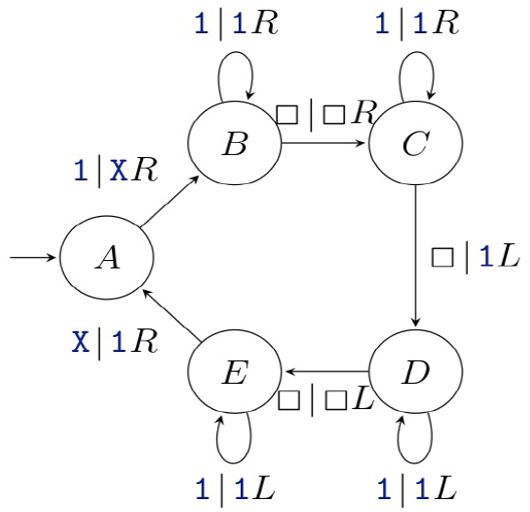
\includegraphics[scale=0.3]{images/turingmaschine_1k.png}
		\end{column}
		
		\begin{column}{0.4\textwidth}
			\begin{description}
				\pause\item[] $\Box (A)11 \Box$
				\pause\item[$\rightarrow$] $\Box X(B)1 \Box$
				\pause\item[$\rightarrow$] $\Box X1(B) \Box$
				\pause\item[$\rightarrow$] $\Box X1 \Box (C) \Box$
				\pause\item[$\rightarrow$] $\Box X1 (D) \Box 1\Box$
				\pause\item[$\rightarrow$] $\Box X (E) 1 \Box 1\Box$
				\pause\item[$\rightarrow$] $\Box (E) X 1 \Box 1\Box$
				\pause\item[$\rightarrow$] $\Box 1 (A) 1 \Box 1\Box$
			\end{description}
		\end{column}
	
		\begin{column}{0.4\textwidth}
			\begin{description}
				\pause\item[$\rightarrow$] $\Box 1 X (B) \Box 1\Box$
				\pause\item[$\rightarrow$] $\Box 1 X \Box (C) 1\Box$
				\pause\item[$\rightarrow$] $\Box 1 X \Box 1 (C)\Box$
				\pause\item[$\rightarrow$] $\Box 1 X \Box (D) 1 1\Box$
				\pause\item[$\rightarrow$] $\Box 1 X (D) \Box 1 1\Box$
				\pause\item[$\rightarrow$] $\Box 1 (E) X \Box 1 1\Box$
				\pause\item[$\rightarrow$] $\Box 1 1 (A) \Box 1 1\Box$
			\end{description}
		\end{column}
	\end{columns}
\end{frame}

\begin{frame}{Halteproblem}
	\markBlue{Halteproblem}: Für einen gegebenen Algorithmus, gelangt dieser bei seiner Abarbeitung zu einem Ende und hält?
	
	\begin{itemize}
		\pitem Algorithmen können durch Turingmaschinen durchgeführt werden
		\pitem Turingmaschinen können durch sogenannte universelle Turingmaschinen simuliert werden
		\begin{itemize}
			\pitem Wenn eine Turingmaschine $T$ kodiert ist mit dem Wort $w$, dann ist $T_w: X \rightarrow X$ eine Funktion, die Eingaben auf die Ausgabe der Turingmaschine $T$ mappt.
			\pitem Also mit $X = \{1,0\}$ gibt z.B. $T_w(100101) = 001$ genau dann zurück, wenn, sofern man $100101$ als Eingabe an die Turingmaschine mit der Kodierung $w$ gibt, diese hält und als Ausgabe $001$ erzeugt.
		\end{itemize}
	\end{itemize}

	\bp
	
	Dann lässt sich das Halteproblem auch als Sprache formulieren:
	
	\vspace{.2cm}
	
	$\quad H = \{w \in A^* : w \text{ ist eine TM-Codierung und } T_w(w) \text{ hält.}\}$
	
	bzw. als allgemeinerer Fall:
	
	$\quad \hat{H} = \{(w,x) \in A^* \times A^* : w \text{ ist eine TM-Codierung und } T_w(x) \text{ hält.}\}$
\end{frame}

\begin{frame}{Halteproblem}
	Das Halteproblem ist unentscheidbar\ip, dh. es gibt keine Turingmaschine, die $H$ entscheidet.
\end{frame}

\begin{frame}{Busy Beaver}
	\markBlue{Busy Beaver TM} ist eine Turingmaschine mit $n$ Zuständen, die möglichst viele Einsen auf das Band schreibt \markBlue{und hält}.
	
	\begin{itemize}
		\pitem Also nicht einfach ewig Einsen aufschreibt und nie aufhört.
	\end{itemize}
	
	\bp
	
	\markBlue{Busy Beaver Problem}: Für eine gegebene Turingmaschine mit $n$ Zuständen, die Einsen aufschreibt und hält: Schreibt sie auch maximal viele Einsen auf?
	
	\bp
	\vspace{.2cm}
	
	Das Busy Beaver Problem ist nicht entscheidbar, bzw. die Busy Beaver Funktion $bb(n)$, die definiert, wieviele einsen von einer Busy Beaver TM maximal geschrieben werden können, ist nicht berechenbar.
	
	\bp
	
	\vspace{.2cm}
	
	Beispielwerte von $bb$: $bb(1) = 1\ip, bb(2) = 4\ip, bb(5) \geq 4098\ip, bb(6) > 10^{18276}$.
\end{frame}

\begin{frame}{Busy Beaver für $n = 3$}
	% 3 zustände und ein haltezustand	
	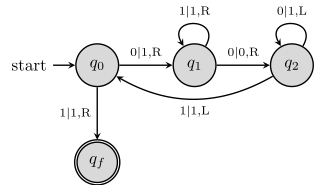
\includegraphics[scale=0.8]{images/turingmaschine_bb.png}	
\end{frame}

\section{Reguläre Ausdrücke}

\begin{frame}{Regulärer Ausdruck}
\begin{block}{Regulärer Ausdruck}
	\begin{itemize}
		\pitem $Z = \{ |, (,), *, \emptyset\}$ Alphabet von ``Hilfssymbolen''
		\pitem Alphabet $A \setminus Z$
		\pitem Ein \textbf{regulärer Ausdruck} (RA) über $A$ ist eine Zeichenfolge über dem Alphabet $A \cup Z$, die gewissen Vorschriften genügt.
		\pitem Vorschriften
		\begin{itemize}
			\pitem $\emptyset$ ist ein RA
			\pitem Für jedes $x \in A$ ist x ein RA
			\pitem Wenn $R_1$ und $R_2$ RA sind, dann auch $(R_1|R_2)$ und $(R_1R_2)$
			\pitem Wenn R ein RA ist, dann auch $(R*)$
		\end{itemize}
	\end{itemize}
\end{block}
\end{frame}

\begin{frame}{Klammerregeln}
\begin{itemize}
\pitem ``Stern- vor Punktrechnung''
\pitem ``Punkt- vor Strichrechnung''
\pitem[$\rightarrow$]$R_1|R_2R_3*$ Kurzform für $(R_1|(R_2(R_3*)))$
\pitem Bei mehreren gleichen Operatoren ohne Klammern links geklammert
\pitem[$\rightarrow$] $R_1|R_2|R_3$ Kurzform für $((R_1|R_2)|R_3)$
\end{itemize}
\pause
\textbf{Aufgabe}\\
Entferne so viele Klammern wie möglich, ohne die Bedeutung des RA zu verändern.\\
\begin{itemize}
\item $(((((ab)b)*)*)|(\emptyset*))$ \pause $\rightarrow$ $(abb)**|\emptyset*$ \pause
\item $((a(a|b))|b)$ \pause  $\rightarrow$ $a(a|b)|b$
\end{itemize}
\end{frame}

\begin{frame}{Alternative Definition}
Wir können die Syntax von regulären Ausdrücken auch über eine kontextfreie Grammatik definieren. \\ \vspace{0.2cm}
\begin{taskblock}{Aufgabe}Vervollständigt die folgende Grammatik.\end{taskblock}
$G = (\{R\}, \{|,(,),*,\emptyset\} \cup A, R, P)$\\
mit $P =\{R\rightarrow \emptyset, R \rightarrow \pause x \text{ }(\text{mit } x \in A),$\\$
R \rightarrow (R|R), R \rightarrow (RR),$\\$
R \rightarrow(R*)$\\$
R \rightarrow \epsilon\}$

\pause

\vspace{.4cm} 
Wieso brauchen wir $\epsilon$?
\end{frame}

\begin{frame}{Durch R beschriebene Sprache}
\textbf{Notation}\\
\begin{itemize}
\item Spitze Klammern $\langle , \rangle$
\end{itemize}

\pause

\textbf{Regeln}\\
%Hier vielleicht selbst auf die Regeln kommen lassen		
\begin{itemize}
\item $\langle \emptyset \rangle = \pause \{\}$ \pause
\item $\langle x \rangle = \pause \{x\}$ für jedes $x \in A$ \pause
\item $\langle R_1| R_2\rangle = \pause \langle R_1\rangle \cup \langle R_2\rangle$ \pause
\item $\langle R_1 R_1 \rangle = \pause \langle R_1 \rangle \cdot \langle R_2 \rangle$ \pause
\item $\langle R* \rangle = \pause \langle R \rangle *$
\end{itemize}
\end{frame}

\begin{frame}{Charakterisierung regulärer Sprachen}
\begin{block}{Satz}
Für jede formale Sprache $L$ sind äquivalent:
\begin{enumerate}
\item $L$ kann von einem endlichen Akzeptor erkannt werden.
\item $L$ kann durch einen regulären Ausdruck beschrieben werden
\item $L$ kann von einer rechtslinearen Grammatik erzeugt werden.
\end{enumerate}
Solche Sprachen heißten regulär.
\end{block}
\end{frame}

\begin{frame}{Anwendung von regulären Ausdrücken}
\vfill \centering Zum selbst probieren:\\http://regexr.com/\\\vspace{.2cm}Achtung: Reguläre Ausdrücke in praktischer Programmierung funktionieren zwar ähnlich, haben aber eine andere Syntax und können teils mehr!\vfill
\end{frame}

\section{Rechtslineare Grammatiken}
\begin{frame}{Rechtslineare Grammatiken}
\begin{block}{Definition}
Eine rechtslineare Grammatik ist eine reguläre Grammatik $G=(N,T,S,P)$ mit der Einschränkung, dass alle Produktionen die folgende Form haben:
\begin{itemize}
\item $X \rightarrow w$ mit $w \in T^*$ oder
\item $x\rightarrow wY$ mit $w \in T^*$, $Y \in N$
\end{itemize}
\end{block}
\end{frame}

\begin{frame}
\begin{taskblock}{Aufgabe zu rechtslinearen Grammatiken}
Gebe zu $L = \{ w \in \{ 0,1 \}^* | \exists k \in \mathbb{N}_0: Num_2(w) = 2^k + 1 \}$ jeweils einen regulären Ausdruck R und eine rechtslineare Grammatik G an, sodass $L = \langle R \rangle = L(G)$ gilt.
\end{taskblock}
\pause
\textbf{Lösung}\\		
\begin{itemize}
\item $R = (0*10)|(0*1(0)* 1) = \pause 0*10|0*10* 1 $ \pause
\item $G = (\{S,A\}, \{0,1\}, S, \{S \rightarrow0S|10|1A, A \rightarrow 0A|1\})$
\end{itemize}
\end{frame}

\begin{frame}
	
\includegraphics[width=\linewidth]{../images/thatsall.png}
\end{frame}


\end{document}
\def\tutdate{2.11.2017}
\ifdefined\compileall

\begin{frame}\vfill\centering \huge\markGreen{Tutorium vom \tutdate} \vfill\end{frame}

\else
\ifdefined\compiletype
	\documentclass[handout]{beamer}
\else
	\documentclass{beamer}
	\def\compiletype{livebeamer}
\fi

\usepackage{templates/beamerthemekitwide}
%\usepackage{enumitem}

\usepackage[utf8]{inputenc}
\usepackage[T1]{fontenc}
\usepackage[ngerman]{babel}
\usepackage{listings}
\usepackage{hyperref}
\usepackage{graphicx}

\usepackage{amsmath}
\usepackage{amsthm}
\usepackage{amssymb}
\usepackage{polynom}

%\usepackage{ifthen}
%\usepackage{adjustbox} % for \adjincludegraphics

%\usepackage{tikz}
\usepackage{listings}

%\usepackage[]{algorithm2e}

%\usepackage{colortbl}
\usepackage{verbatim}
%\usepackage{alltt}
%\usepackage{changes}

%\usepackage{pdfpages}
%\usepackage{tabularx}

%\usepackage{euler}


\newcommand{\markBlue}[1]{\textcolor{kit-blue100}{#1}}
\newcommand{\markGreen}[1]{\textcolor{kit-green100}{#1}}
\newcommand{\vertspace}{\vspace{.2cm}}

%\newcommand{\#}{\markBlue{#1}}

%\newcommand{\pitem}{\pause\item}
\newcommand{\p}{\pause}

% -- MATH MACROS
\newcommand{\thistheoremname}{}
\newcommand{\G}{\mathbb{Z}}
\newcommand{\B}{\mathbb{B}}
\newcommand{\R}{\mathbb{R}}
\newcommand{\N}{\mathbb{N}}
\newcommand{\Q}{\mathbb{Q}}
\newcommand{\C}{\mathbb{C}}
\newcommand{\Z}{\mathbb{Z}}
\newcommand{\F}{\mathbb{F}}
\newcommand{\mi}{\mathrm{i}}
\renewcommand{\epsilon}{\varepsilon}
\newcommand{\okalk}{\mathscr{O}}


\newenvironment<>{taskblock}[1]{%
	\setbeamercolor{block title}{fg=kit-orange15,bg=kit-orange100}
	\setbeamercolor{block body}{fg=black,bg=kit-orange30}%
	\begin{block}#2{#1}}{\end{block}}

\setbeamertemplate{enumerate items}[default]

% Aussagenlogik Symbole
\newcommand{\W}{w}
\renewcommand{\F}{f}

% Kodierung
\newcommand{\frepr}{\textbf{repr}}
\newcommand{\fRepr}{\textbf{Repr}}
\newcommand{\fZkpl}{\textbf{Zkpl}}
\newcommand{\fbin}{\textbf{bin}}
\newcommand{\fdiv}{\textbf{ div }}
\newcommand{\fmod}{\textbf{ mod }}

% Speicherabbild
\newenvironment{memory}{\begin{tabular}{r | l}Adresse&Wert\\\hline\hline}{\end{tabular}}
\newcommand{\memrow}[2]{#1 & #2 \\\hline}

% Praedikatenlogik
\newcommand{\objequiv}{\stackrel{\cdot}{=}}
\newcommand{\pval}{val_{D,I,\beta}}

% Neue Befehle
\newcommand{\ip}{\pause} % inline pause, für mitten im satz
\newcommand{\pitem}{\pause\item} % für aufzählungen
\newcommand{\bp}{\pause} % block pause, für zwischen blöcken

\title[Grundbegriffe der Informatik]{Grundbegriffe der Informatik\\Tutorium 36}
\date{\tutdate}
\subtitle{}
\author{Maximilian Staab, \texttt{uxhdf@student.kit.edu}}



\institute{}

%\titlelogo{lukasbach}

\titleimage{bg}
%\titleimage{bg-advent}


\ifthenelse{\equal{\compiletype}{livebeamer}}
	{
		\def\livebeamermode{1}
	}{}

\ifthenelse{\equal{\compiletype}{print}}
	{
		\def\printmode{1}
	}{}

\setbeamercovered{invisible}

%\usepackage[citestyle=authoryear,bibstyle=numeric,hyperref,backend=biber]{biblatex}
%\addbibresource{templates/example.bib}
%\bibhang1em

\begin{document}
	
\selectlanguage{ngerman}


%title page
\begin{frame}
	\titlepage
\end{frame}

%table of contents
\ifdefined\printmode
	\ifdefined\compileall \else
	\begin{frame}{Gliederung}
		\tableofcontents
	\end{frame}
\fi\fi

\fi

\section{Wiederholung und Übung}
\begin{frame}{Maß für Information}
	Die Zahl der verschiedenen mäglichen Nachrichten ist ein Maß für die\\
	Information einer Nachricht, wenn das Auftreten der Nachrichten\\
	 gleichverteilt ist.
	 \begin{itemize}
		 \item Logarithmus naturalis: natural units (nat)
		 \item Logarithmus zur Basis 10: Hartley (Hart)
		 \item Logarithmus dualis: Shannon (Sh)
	 \end{itemize}
\end{frame}

\begin{frame}{Mengen}
	Seien $A=\{1,2,3,4\}, B=\{3.4.5.6.7\}, C=\{5,6,7\}$. Bestimme
	\begin{itemize}
		\item $A \cup B$
		\item $A \cup C$
		\item $A \cap B$
		\item $A \cap C$
	\end{itemize}
	sowie die Kardinalität dieser Mengen.
\end{frame}
\begin{frame}{Mengen}
	Lösung:
	\begin{itemize}
		\item $A \cup B = \{1,2,3,4,5,6,7,\}$ und $\mid A \cup B\mid = 7$
		\pause
		\item $A \cup B = \{1,2,3,4,5,6,7,\}$ und $\mid A \cup C\mid = 7$
		\pause
		\item $A \cap B = \{3,4\}$ und $\mid A \cap B \mid = 2$
		\pause
		\item $A \cap C = \emptyset$ und $\mid\emptyset\mid = 0$
	\end{itemize}
\end{frame}

\begin{frame}{Mengen}
	\begin{block}{Aufgabe aus WS16/17}
		Es seinen A,B und C Mengen. Beweisen oder widerlegen Sie:
		$A \backslash (B \backslash C) = (A \backslash B)\backslash C$
	\end{block}
	\pause
	\begin{block}{Widerlegung durch Gegenbeispiel}
		Seien $A = \{1,2,3\}, B = \{3,4,5\}$ und $C = \{3\}$.
		Dann ist $\{1,2,3\} \backslash (\{3,4,5\} \backslash \{3\}) = \{1,2,3\} \backslash \{4,5\} = \{1,2,3\} \neq$
		$\{1,2\} = \{1,2\} \backslash \{3\} = (\{1,2,3\} \backslash \{3,4,5\}) \backslash \{3\}$
	\end{block}
\end{frame}
\begin{frame}{Mengenäquivalenz}
	\begin{block}{Zeigen Sie}
		$A \cup (B \cap C) = (A \cup B) \cap (A \cup C)$
		\begin{itemize}
			\pause\item ``$\subseteq$'': Sei $x \in A \cup (B\cap C).$ Dann ist $x \in A$ oder $x \in (B \cap C)$
			\begin{itemize}
				\pause
				\item Falls $x\in A$, dann gilt auch $x\in (A\cup B)$ und $x\in (A\cup C)$. Also
				insbesondere $x\in(A\cup B)\cap(A\cup C)$.
				\pause
				\item Falls $x\in(B\cap C)$, dann gilt auch $x\in (A\cup B)$ und $x\in (B\cup C)$. Also
				insbesondere $x\in(A\cup B)\cap(A\cup C)$.
				\pause
			\end{itemize}
			\item ``$\supseteq$'': $x\in(A\cup B)\cap(A\cup C)$. Dann liegt x in $(A\cup B)$ und $(A\cup C)$.
			Also liegt x entweder in A oder in (B und C). Folglich gilt 
			$x\in A\cup(A\cap C)$.
			\pause\item Insgesamt ist also $A\cup(B\cap C) = (A\cup B)\cap(A\cup C)$.
		\end{itemize}
	\end{block}
\end{frame}

\begin{frame}{Mengen}
	\begin{block}{Aufgabe aus WS16/17}
		Es sei M eine Menge und es seien $A\subseteq M$ und $B\subseteq M$. Beweisen Sie:
		$M\backslash(A\cap B) = (M\backslash A)\cup(M\backslash B)$
		\begin{itemize}
			\pause \item ``$\subseteq$'': Sei $x\in M\backslash(A\cap B)$. Dann ist $x\in M$ und $x\notin A$ oder $x\notin B$.
			\\Somit ist
			\begin{itemize}
				\item $x\in M$ und $x\notin A$ oder
				\item $x\in M$ und $x\notin B$.
			\end{itemize}
			Also ist $x\in(M\backslash A)$ oder $(M\backslash B)$, folglich also
			$x\in(M\backslash A)\cup(M\backslash B)$.

			\pause\item ``$\supseteq$'': Sei $x\in(M\backslash A)\cup(M\backslash B)$. Dann ist $x\in(M\backslash A)$ oder\\
			$x\in(M\backslash B)$. Somit ist
			\begin{itemize}
				\item $x\in M$ und $x\notin A$ oder
				\item $x\in M$ und $x\notin B$.
			\end{itemize}
			Also ist $x\in M$, und $x\notin A$ oder $x\notin B$. Dann ist $x\in M$ und \\
			$x\notin(A\cap B)$, folglich also $x\in M\backslash(A\cap B)$.
		\end{itemize}
	\end{block}
\end{frame}

\section{Wörter}

\begin{frame}{Wörter}
	\begin{block}{Konkatenation}
		Durch Konkatenation werden einzelne Buchstaben aus einem Alphabet miteinander verbunden.
	\end{block}

	\begin{itemize}
		\pitem Symbol: $\cdot$\pause , also zwei Buchstaben $a$ und $b$ miteinander konkateniert: $a \cdot b$.
		\pitem Nicht kommutativ : $a \cdot b \neq b \cdot a$
		\pitem Aber assoziativ : $(a \cdot b) \cdot c = a \cdot (b \cdot c)$
		\pitem Kurzschreibweise : Ohne Punkte , also $a \cdot b = ab$
	\end{itemize}
\end{frame}

\begin{frame}{Wörter}
	\begin{block}{Wörter: Intuitivere Definition}
		Ein Wort $w$ entsteht durch die Konkatenation durch Buchstaben aus einem Alphabet.
	\end{block}

	$\rightarrow$ Also Abfolge von Zeichen über ein Alphabet A.

	\pause Sei $A := \{a, b, c\}$.

	\begin{itemize}
		\pitem Mögliche Worte: \pause $w_1 := a \cdot b$\pause , $w_2 = b \cdot c \cdot c$\pause , $w_3 = a \cdot c \cdot c \cdot b \cdot a$.
		\pitem Keine möglichen Worte: \pause $d$.
		\end{itemize}
\end{frame}

\begin{frame}{Wörter}
	\begin{block}{Wörter: Abstraktere Definition}
		Ein Wort $w$  über dem Alphabet $A$  ist definiert als surjektive Abbildung  $w : \Z_n \rightarrow A$. Dabei heißt $n$ die Länge $|w|$ des Wortes.
	\end{block}

	\begin{itemize}
		\pitem $\Z_n$  $ = \{i \in \N : 0 \leq i < n \}$
		
		\pause $\Z_3  = \{0, 1, 2\},  \Z_2 = \{0, 1\}, \Z_0 = \emptyset$.
		
		\pitem Länge oder Kardinalität eines Wortes:  $|w|$. \pause $|abcde|$ $= 5$.
		
		\pitem Wort $w = abdec$ als Relation aufgeschrieben: \pause $w = \{(0, a), (1, b), (2, d), (3, e), (4, c)\}$.  Also $w(0) = a, w(1) = b, w(2) = d, \dots$
		
		\pause Damit sieht man auch: $|w| = |\{(0, a), (1, b), (2, d), (3, e), (4, c)\}| = 5$.
	\end{itemize}
\end{frame}

\begin{frame}{Wörter}
	\begin{itemize}
		\item Wort der Kardinalität 0?
	\end{itemize}

	\pause

	\begin{block}{Das leere Wort}
		Das leere Wort $\varepsilon$ ist definiert ein Wort mit Kardinalität 0 , also mit 0 Zeichen.
	\end{block}

	\begin{itemize}
		\pitem Leere Wort wird interpretiert als ``nicht sichtbar'' und kann überall platziert werden\pause : $aabc = a\epsilon abc = \epsilon\epsilon a\epsilon bc \epsilon$.
		\pitem $|\{\epsilon\}|$ \pause $ = 1$ , die Menge ist nicht leer! Das leere Wort ist nicht \emph{nichts}! (Vergleiche leere Menge)
		\pitem $|\epsilon| = 0$.
	\end{itemize}
\end{frame}

\begin{frame}{Mehr über Wörter}
	\begin{block}{$A^n$}
		Zu einem Alphabet $A$ ist $A^n$ definiert als die Menge aller Wörter der Länge $n$ über dem Alphabet $A$.
	\end{block}

	\begin{itemize}
		\pitem Nicht mit Mengenpotenz verwechseln!
		\pitem $A := \{a, b, c\}$\pause , $A^2 = \{aa, ab, ac, ba, bb, bc, ca, cb, cc\}$. \pause $A^1 = A, \pause A^0 = \{\epsilon\}$.
	\end{itemize}
	
	\pause Die Menge aller Wörter  \emph{beliebiger} Länge: \pause
	\begin{itemize}
		\item $A^* := \bigcup_{i \in \N_0} A_i$
		\pitem $A := \{a, b, c\}$ . $aa \in A^* , abcabcabc \in A^* , aaaa \in A^* , \epsilon \in A^*$.
	\end{itemize}
\end{frame}

\begin{frame}{Mehr über Wörter}
	\begin{block}{Wort Potenzen}
		Sich direkt wiederholende Teilworte kann man als Wortpotenz darstellen , daher $w_i^n = w_i \cdot w_i \cdots w_i$ (n $\times$ mal).
	\end{block}

	\begin{itemize}
		\pitem $a^4 = aaaa$\pause , $b^3 = bbb$\pause , $c^0 = \pause \epsilon$\pause , $d^1 = \pause d$.
		\pitem $a^3c^2b^6 \pause = aaaccbbbbbb$.
		\pitem $b \cdot a \cdot (n \cdot a)^2$ \pause $ = banana$.
		\end{itemize}
\end{frame}

\begin{frame}{Übung zu Wörter}
	Sei $A$ ein Alphabet.
	
	\begin{taskblock}{Übung zu Wörter}
		\begin{enumerate}
			\item Finde Abbildung $f: A^* \rightarrow A^*$, sodass für alle $w \in A^*$ gilt: \\\quad $2 \cdot |w| = |f(w)|$.
			\item Finde Abbildung $g: A^* \rightarrow A^*$, sodass für alle $w \in A^*$ gilt: \\\quad $|w| + 1 = |g(w)|$.
			\item Sind $f, g$ injektiv und/oder surjektiv?
		\end{enumerate}
	\end{taskblock}

	\pause
	
	\begin{enumerate}
		\item $f: A^* \rightarrow A^*, w \mapsto w \cdot w$.
		\pitem $g: A^* \rightarrow A^*, w \mapsto w \cdot x, x \in A$.
	\end{enumerate}
\end{frame}

\begin{frame}{Übung zu Wörter}
	\begin{enumerate}
		\item $f: A^* \rightarrow A^*, w \mapsto w \cdot w$.
		\begin{itemize}
			\pitem $f$ ist injektiv\pause , denn jedes $w$ aus der Bildmenge wird von maximal einem Wort abgebildet.
			\pitem $f$ ist nicht surjektiv\pause , denn z.B. bildet nichts auf $x \in A$ ab (oder auf andere Wörter mit ungerader Anzahl an Buchstaben).
		\end{itemize}
		\pitem $g: A^* \rightarrow A^*, w \mapsto w \cdot x, x \in A$.
		\begin{itemize}
			\pitem $g$ ist injektiv.
			\pitem $g$ ist nicht surjektiv\pause , denn z.B. bildet nichts auf $\epsilon$ ab.
		\end{itemize}
	\end{enumerate}
\end{frame}

\section{Formale Sprachen}

\begin{frame}{Formale Sprache}
	\begin{itemize}
		\pitem Was war nochmal $A^*$? Menge aller Wörter \emph{beliebiger} Länge über Alphabet $A$.
	\end{itemize}

	\pause
	
	\begin{block}{Formale Sprache}
		Eine Formale Sprache $L$ über einem Alphabet $A$ ist eine Teilmenge $L \subseteq A^*$.
	\end{block}

	\begin{itemize}
		\pitem Zufälliges Beispiel: \pause $A := \{b, n, a\}$.
		\begin{itemize}
			\pitem $L_1 := \{ban, baan, nba, aa\}$ ist eine mögliche formale Sprache über $A$.
			\pitem $L_2 := \{banana, bananana, banananana, ...\}$ \pause $ = \{w : w = bana(na)^k, k \in \N\}$ auch.
			\pitem $L_3 := \{ban, baan, baaan, ...\}$ auch. \pause Andere Schreibweise? \pause \\ $ L_3 = \{w : w = ba^kn, k \in \N \}$
		\end{itemize}
		\pitem Formale Sprachen sind also nicht zwangsweise endliche Mengen.
		\pitem Praktischeres Beispiel: $A := \{w : w $ ist ein ASCII Symbol $\}$.
		\begin{itemize}
			\pitem $L_4 := \{class, if, else, while, for, ...\}$ ist eine formale Sprache über $A$.
			\pitem $L_5 := \{w : w = a \cdot b$ mit $a$ als Großbuchstabe und $b$ als Groß- oder Kleinbuchstabe $ \} \pause \backslash L_4$ \pause ist eine formale Sprache von korrekten Klassennamen in Java.
		\end{itemize}
	\end{itemize}
\end{frame}

\begin{frame}{Übung zu formalen Sprachen}
	$A := \{a, b\}$
	
	\begin{itemize}
		\pitem Sprache $L$ aller Wörter über $A$, die nicht das Teilwort $ab$ enthalten?
		\begin{itemize}
			\pitem Was passiert wenn ein solches Wort ein $a$ enthält? \pause Dann keine $b$'s mehr!
			\pitem $L = \{w_1 \cdot w_2 : w_1 \in \{b\}^*$ und $w_2 \in \{a\}^* \}$
			\pitem Andere Möglichkeit\pause : Suche Wörter mit $ab$ und nehme diese Weg.
			\pitem $L = \{a, b\}^*\pause \backslash\{ w_1 \cdot ab \cdot w_2 : w_1, w_2 \in \{a,b\}^* \}$
		\end{itemize}
	\end{itemize}
\end{frame}

\begin{frame}{Übung zu formalen Sprachen}
	
	Sei $A := \{a, b\}, B := \{0, 1\}$.
	
	\begin{taskblock}{Aufgabe zu formalen Sprachen}
		\begin{enumerate}
			\item Sprache $L_1 \subseteq A^*$ von Wörtern, die mindestens drei $b$'s enthalten.
			\item Sprache $L_2 \subseteq A^*$ von Wörtern, die gerade Zahl von $a$'s enthält.
			\item Sprache $L_3 \subseteq B^*$ von Wörtern, die, interpretiert als Binärzahl eine gerade Zahl sind.
		\end{enumerate}
	\end{taskblock}

	\pause
	
	\begin{enumerate}
		\item $L_1 = \{w = w_1  b  w_2  b  w_3 b w_4 : w_1,w_2,w_3,w_4 \in A^* \}$
		\pitem $L_2 = \{w = (w_1 a w_2 a w_3)^* : w_1,w_2,w_3 \in \{b\}^* \}$ \pause (Ist da $\epsilon$ drin?)
		\pitem $L_3 = \{w = w \cdot 0 : w \in B^* \}$
	\end{enumerate}
\end{frame}

\ifdefined\compileall
\else


\ifthenelse{\equal{\compiletype}{print}}
{

\begin{frame}{Informationen}
	
	\begin{columns}
		\begin{column}{0.5\textwidth}
			
			\begin{block}{Zum Tutorium}
				\begin{itemize}
					\item Maximilian Staab
					\item Tutoriumsnummer: 36
					\item Tutorium findet statt:
					\begin{itemize}
						\item Donnerstags, 09:45 - 11:15
						\item 50.34 Informatikbau, -109
					\end{itemize}
				\end{itemize}
			\end{block}
			
			\begin{block}{Mehr Material}
				\begin{itemize}
					\item Ehemalige GBI Webseite:
					\begin{itemize}
						\item \url{http://gbi.ira.uka.de}
						\item Altklausuren!
					\end{itemize}
				\end{itemize}
			\end{block}
			
		\end{column}
		\begin{column}{0.5\textwidth}
			
			\begin{block}{Zur Veranstaltung}
				\begin{itemize}
					\item Grundbegriffe der Informatik
					\item Klausurtermin:
					\begin{itemize}
						\item 08.03.2018, 14:00
						\item Zwei Stunden Bearbeitungszeit
						\item 6 ECTS für Informatiker und Informationswirte, 4 ECTS für ?
					\end{itemize}
				\end{itemize}
			\end{block}
			
			\begin{block}{Zum Übungsschein}
				\begin{itemize}
					\item Übungsblatt alle zwei wochen
					\item Ab >50\% insgesamt hat man den Übungsschein
					\item Keine Voraussetzung für die Klausur, aber für das Modul
				\end{itemize}
			\end{block}
			
		\end{column}
	\end{columns}
	
\end{frame}

}{}

\ifdefined\livebeamermode
	\begin{frame}
		
\includegraphics[width=\linewidth]{images/thatsall.png}
	\end{frame}
\fi

\end{document}

\fi
\def\tutdate{09.11.2017}
\ifdefined\compileall

\begin{frame}\vfill\centering \huge\markGreen{Tutorium vom \tutdate} \vfill\end{frame}

\else
\ifdefined\compiletype
	\documentclass[handout]{beamer}
\else
	\documentclass{beamer}
	\def\compiletype{livebeamer}
\fi

\usepackage{templates/beamerthemekitwide}
%\usepackage{enumitem}

\usepackage[utf8]{inputenc}
\usepackage[T1]{fontenc}
\usepackage[ngerman]{babel}
\usepackage{listings}
\usepackage{hyperref}
\usepackage{graphicx}

\usepackage{amsmath}
\usepackage{amsthm}
\usepackage{amssymb}
\usepackage{polynom}

%\usepackage{ifthen}
%\usepackage{adjustbox} % for \adjincludegraphics

%\usepackage{tikz}
\usepackage{listings}

%\usepackage[]{algorithm2e}

%\usepackage{colortbl}
\usepackage{verbatim}
%\usepackage{alltt}
%\usepackage{changes}

%\usepackage{pdfpages}
%\usepackage{tabularx}

%\usepackage{euler}


\newcommand{\markBlue}[1]{\textcolor{kit-blue100}{#1}}
\newcommand{\markGreen}[1]{\textcolor{kit-green100}{#1}}
\newcommand{\vertspace}{\vspace{.2cm}}

%\newcommand{\#}{\markBlue{#1}}

%\newcommand{\pitem}{\pause\item}
\newcommand{\p}{\pause}

% -- MATH MACROS
\newcommand{\thistheoremname}{}
\newcommand{\G}{\mathbb{Z}}
\newcommand{\B}{\mathbb{B}}
\newcommand{\R}{\mathbb{R}}
\newcommand{\N}{\mathbb{N}}
\newcommand{\Q}{\mathbb{Q}}
\newcommand{\C}{\mathbb{C}}
\newcommand{\Z}{\mathbb{Z}}
\newcommand{\F}{\mathbb{F}}
\newcommand{\mi}{\mathrm{i}}
\renewcommand{\epsilon}{\varepsilon}
\newcommand{\okalk}{\mathscr{O}}


\newenvironment<>{taskblock}[1]{%
	\setbeamercolor{block title}{fg=kit-orange15,bg=kit-orange100}
	\setbeamercolor{block body}{fg=black,bg=kit-orange30}%
	\begin{block}#2{#1}}{\end{block}}

\setbeamertemplate{enumerate items}[default]

% Aussagenlogik Symbole
\newcommand{\W}{w}
\renewcommand{\F}{f}

% Kodierung
\newcommand{\frepr}{\textbf{repr}}
\newcommand{\fRepr}{\textbf{Repr}}
\newcommand{\fZkpl}{\textbf{Zkpl}}
\newcommand{\fbin}{\textbf{bin}}
\newcommand{\fdiv}{\textbf{ div }}
\newcommand{\fmod}{\textbf{ mod }}

% Speicherabbild
\newenvironment{memory}{\begin{tabular}{r | l}Adresse&Wert\\\hline\hline}{\end{tabular}}
\newcommand{\memrow}[2]{#1 & #2 \\\hline}

% Praedikatenlogik
\newcommand{\objequiv}{\stackrel{\cdot}{=}}
\newcommand{\pval}{val_{D,I,\beta}}

% Neue Befehle
\newcommand{\ip}{\pause} % inline pause, für mitten im satz
\newcommand{\pitem}{\pause\item} % für aufzählungen
\newcommand{\bp}{\pause} % block pause, für zwischen blöcken

\title[Grundbegriffe der Informatik]{Grundbegriffe der Informatik\\Tutorium 36}
\date{\tutdate}
\subtitle{}
\author{Maximilian Staab, \texttt{uxhdf@student.kit.edu}}



\institute{}

%\titlelogo{lukasbach}

\titleimage{bg}
%\titleimage{bg-advent}


\ifthenelse{\equal{\compiletype}{livebeamer}}
	{
		\def\livebeamermode{1}
	}{}

\ifthenelse{\equal{\compiletype}{print}}
	{
		\def\printmode{1}
	}{}

\setbeamercovered{invisible}

%\usepackage[citestyle=authoryear,bibstyle=numeric,hyperref,backend=biber]{biblatex}
%\addbibresource{templates/example.bib}
%\bibhang1em

\begin{document}
	
\selectlanguage{ngerman}


%title page
\begin{frame}
	\titlepage
\end{frame}

%table of contents
\ifdefined\printmode
	\ifdefined\compileall \else
	\begin{frame}{Gliederung}
		\tableofcontents
	\end{frame}
\fi\fi

\fi


\section{Aussagenlogik}

\begin{frame}{Aussagenlogik}
	\begin{itemize}
		\pitem Das wars erst mal zu formalen Sprachen.
		\pitem Heute ist Donnerstag.
		\pitem Die Menge aller Männer dieser Welt ist disjunkt zur Menge aller Frauen dieser Welt.
	\end{itemize}

	\pause
	
	Das sind alles Aussagen. Aussagen sind entweder \emph{wahr} oder \emph{falsch}.
\end{frame}

\begin{frame}{Aussagenlogik}
	
	Wir kapseln Aussagen und verwendet Variablen dafür. 
	
	Zum Beispiel:
	
	\begin{itemize}
		\pitem $A := $ ``Die Straße ist nass.''
		\pitem $B := $ ``Es regnet.''
	\end{itemize}

	\pause Aussagen lassen sich verknüpfen:
	
	\begin{itemize}
		\pitem \markGreen{Logisches Und:} $A \land B = A$ und $B = $ Die Straße ist nass und es regnet.
		\pitem \markGreen{Logisches Oder:}  $A \lor B  = A$ oder $B  = $ Die Straße ist nass oder es regnet . Es kann auch beides wahr sein.
		\pitem \markGreen{Negierung:}  $\lnot A  = $ nicht $A  = $ Die Straße ist nicht nass.
		\pitem \markGreen{Implikation:}  $A \rightarrow B  = $ Aus $A$ folgt $B  = $ Wenn die Straße nass ist, dann regnet es.
		\pitem \markGreen{Äquivalenz:}pause $A \leftrightarrow B  = A$ und $B$ sind äquivalent $ = $ Die Straße ist \emph{genau dann} nass, \emph{wenn} es regnet.
		\begin{itemize}
			\pitem $A \leftrightarrow B = (A \rightarrow B) \land (B \rightarrow A)$  , also die Straße ist nass wenn es regnet \emph{und} es regnet wenn die Straße nass ist.
		\end{itemize}
	\end{itemize}

\end{frame}

\begin{frame}{Übung zu Aussagenlogik}
	
	\begin{itemize}
		\item $A := $ ``Die Straße ist nass.''
		\item $B := $ ``Es regnet.''
		\item $C := $ ``$\pi$ ist gleich $3$.''
	\end{itemize}

	\begin{itemize}
		\pitem Was ist $B \rightarrow C$?   ``Wenn es regnet, ist $\pi$ gleich $3$.''
	\end{itemize}

	\pause
	
	% Aus Skriptum, Kapitel 5.3 Boolesche Funktionen
	\begin{center}
		\begin{tabular}{c|c||c|c|c|c}%*{2}{>{$}c<{$}}|*{4}{>{$}c<{$}}
			\hline
			$x_1$ & $x_2$ & $\lnot x_1$ & $x_1 \land x_2$ & $x_1 \lor x_2$ & $x_1 \rightarrow x_2$ \\
			\hline
			\F & \F & \W & \F & \F & \W \\
			\F & \W & \W & \F & \W & \W \\
			\W & \F & \F & \F & \W & \F \\
			\W & \W & \F & \W & \W & \W \\
			\hline
		\end{tabular}
	\end{center}
	
\end{frame}

\begin{frame}{Syntax der Aussagenlogik}
	\pause
	Menge der Aussagevariablen:
	
	\pause\quad $Var_{AL} \pause \subseteq \{P_i : i \in \N_0\}$ \pause oder $\{P, Q, R, S, \dots\}$
	
	\pause Alphabet der Aussagenlogik:
	
	\pause\quad $A_{AL} = \{(, ), \lnot, \land, \lor, \rightarrow, \leftrightarrow\} \cup Var_{AL}$
\end{frame}

\begin{frame}{Boolesche Funktionen}
\begin{block}{Boolesche Funktionen}
	Eine boolsche Funktion ist eine Abbildung \pause der Form $f: \B^n \rightarrow \B$ \pause mit $\B = \{w, f\}$.
\end{block}

Typische Boolsche Funktionen\pause : $b_\lnot (x) \pause = \lnot x$\pause , $b_\lor (x_1, x_2) \pause = x_1 \lor x_2$ \dots
\end{frame}

\begin{frame}{Interpretationen}
	\begin{block}{Interpretation}
		\pause Eine Interpretation ist eine Abbildung $I : V \rightarrow \B$\pause , die einer Variablenmenge eine ``Interpretation''\pause , also wahr oder falsch zuordnet.
	\end{block}

\pause Weiter legt man $val_I(F)$ als Auswertung einer aussagenlogischer Formel $F$ fest.
\pause
	\newcommand{\val}{val}
	\begin{align*}
	\val_I(X)         &= I(X) \\
	\val_I(\lnot G)   &= b_{\lnot}(\val_I(G)) \\
	\val_I(G \land H) &= b_{\land}(\val_I(G), \val_I(H)) \\
	\val_I(G \lor H)  &= b_{\lor}(\val_I(G)  \val_I(H)) \\
	\val_I(G \rightarrow H)&= b_{\rightarrow}(\val_I(G), \val_I(H))
	\end{align*}
\end{frame}

\begin{frame}{Übung zu Interpretationen}
	
	
	\begin{itemize}
		\item Wie viele Interpretationen gibt es bei k = 1, 2, 3 Variablen?
		\item Wie viele Interpretationen gibt es bei k+1 Variablen im Vergleich zu k Variablen?
	\end{itemize}
	
\end{frame}	

\begin{frame}{Übung zur Aussagenlogik}
	\pause Sei $A := \W, B := \W, C := \F$.
	
	\begin{itemize}
		\pitem Ist $(A \land B) \lor \lnot C$ wahr oder falsch? \pause $(A \land B) \lor \lnot C \pause = (\W \land \W) \lor \lnot \F \pause = \W \lor \lnot \F = \pause \W \lor \W \pause = \W$\pause , die Aussage ist also wahr.
		\pitem Ist $\lnot (A \lor A)$ wahr oder falsch? \pause Falsch! \pause Wann ist $\lnot (A \lor A)$ im allgemeinen wahr? \pause Genau dann, wenn $\lnot A$ wahr ist.
	\end{itemize}

	\pause

	\begin{block}{Äquivalenz von Aussagen}
		Erinnerung: \pause $A \leftrightarrow B$ heißt: \pause $(A \rightarrow B) \land (B \rightarrow A)$. 
		
		\pause Wenn zwei Aussagen äquivalent sind, sind ihre Wahrheitswerte immer gleich\pause , wenn die Wahrheitswerte, von denen sie abhängen, gleich sind. 
		
		\pause Mann sagt und schreibt dann: \pause $A$ ist \emph{genau dann} wahr, \emph{wenn} $B$ wahr ist.
	\end{block}

	\begin{itemize}
		\pitem $\lnot (A \lor A)$ ist genau dann wahr\pause , wenn $\lnot A$ wahr ist\pause , also gilt:  $\lnot (A \lor A) \pause \leftrightarrow \lnot A$. 
	\end{itemize}
\end{frame}

\begin{frame}{Mehr zu Äquivalenz}
\pause
	\begin{block}{Alternative Definition zu Äquivalenz}
		Zwei Formeln G und H heißen äquivalent, wenn für jede Interpretation gilt $val_I(G) = val_I(H)$.
	\end{block}\pause

	Vorher Äquivalenz von Formeln unter gegebener Interpretation\pause , diesmal Äquivalenz von Formeln unter beliebiger Interpretation.\pause

	\textbf{Bemerkung}\\
	\begin{itemize}
		\pitem Man schreibt $G \equiv  H$
		\pitem $\mathbb{B}^V \rightarrow \mathbb{B}: I \mapsto val_I(G)$
	\end{itemize}\pause
	\textbf{Beispiele}\\\pause
	$(\lnot(\lnot P))$ ist äquivalent zu $P$\\\pause
	$(\lnot(P\land Q))$ ist äquivalent zu $((\lnot P) \lor (\lnot Q))$
\end{frame}

\begin{frame}{Beispiele zu Äquivalenz}
	\begin{itemize}
		\pitem Ein Wort $w$ hat die Länge $n$ $\leftrightarrow |w| = n$.
		\pitem Die Vereinigung zweier Mengen $A$ und $B$ hat die Kardinalität $|A| + |B|$ \pause $\leftrightarrow$ $A \cap B = \emptyset$ \pause $\leftrightarrow$ $A$ und $B$ sind disjunkt.
		\pitem $p$ ist eine rationale Zahl \pause $\leftrightarrow$ $p$ lässt sich darstellen als $p = \frac{a}{b}, a\in \Z, b \in \N$ \pause $\leftrightarrow$ $p \in \Q$.
	\end{itemize}	
\end{frame}

\begin{frame}{Wahrheitstabellen}
	\begin{itemize}
		\item $(((P \land Q) \lor Q) \rightarrow (P \land \lnot Q))$
	\end{itemize}

	\begin{center}
		\begin{tabular}{c|c||c|c|c|c}%*{2}{>{$}c<{$}}|*{4}{>{$}c<{$}}
			\hline
				$P$ & $Q$ & $(P \land Q)$ & $\lor Q$ & $\rightarrow$ & $(P \land \lnot Q)$ \\\hline
				
				\visible<1->{\W} & \visible<1->{\W} & \visible<2->{\W} & \visible<6->{\W} & \visible<14->{\F} & \visible<10->{\F} \\\hline
				
				\visible<1->{\W} & \visible<1->{\F} & \visible<3->{\F} & \visible<7->{\F} & \visible<15->{\W} & \visible<11->{\W} \\\hline
				
				\visible<1->{\F} & \visible<1->{\W} & \visible<4->{\F} & \visible<8->{\W} & \visible<16->{\F} & \visible<12->{\F} \\\hline
				
				\visible<1->{\F} & \visible<1->{\F} & \visible<5->{\F} & \visible<9->{\F} & \visible<17->{\W} & \visible<13->{\F} \\\hline
				
		\end{tabular}
	\end{center}
\end{frame}

\begin{frame}{Übungen zu Aussagenlogik}
	\begin{taskblock}{Übungen zu Aussagenlogik}
		\begin{itemize}
			\item Schreibe Wahrheitstabellen zu den Formeln um den Wahrheitsgehalt festzustellen.
				\item $\lnot(P \land Q) \land \lnot (Q \land P)$
				\item $(P \land Q \land R) \leftrightarrow (\lnot P \lor Q)$
				\item $(A\land(B\lor C))\leftrightarrow ((A\land B)\lor(A\land C))$
			\item Welche dieser Aussagen sind wahr?
				\item $\lnot (P \land Q) = \lnot P \lor \lnot Q$
				\item $P \land P = P \lor P$
				\item $(P \lor Q) \land R = (P \land R) \lor (Q \land R)$
		\end{itemize}
	\end{taskblock}
\end{frame}

\begin{frame} {Wahrheitstabellen}
	\begin{center}
		\begin{tabular}{|c|c|c|c|c|c|c|}
			\hline
			$A$&$B$& $\lnot A$& $A \land B$ & $A\lor B$ &$A\rightarrow B$ &$A \leftrightarrow B$\\
			\hline
			w&w&f&w&w&w&w\\
			w&f&f&f&w&f&f\\
			f&w&w&f&w&w&f\\
			f&f&w&f&f&w&w\\
			\hline
		\end{tabular}
	\end{center}

	\begin{taskblock}{Aufgabe}
		Finde einen logischen Ausdruck in A und B unter Verwendung von $\land, \lor$ und $\lnot$, der die Aussage ``Entweder A oder B'' repräsentiert	
	\end{taskblock}
\end{frame}

\begin{frame}{Wahrheitstabellen}
	
	\begin{taskblock}{Aufgabe}
		Finde einen logischen Ausdruck in A und B unter Verwendung von $\land, \lor$ und $\lnot$, der die Aussage ``Entweder A oder B'' repräsentiert	
	\end{taskblock}

	\textbf{Lösung}
	\begin{center}
		\begin{tabular}{|c|c|c|c|c|}
			\hline
			$A$&$B$& $A \land \lnot B$& $\lnot A \land B$ & $(A \land \lnot B) \lor (\lnot A \land B) $\\
			\hline
			w&w&f&f&f\\
			w&f&w&f&w\\
			f&w&f&w&w\\
			f&f&f&f&f\\
			\hline
		\end{tabular}
	\end{center}
\end{frame}


\begin{frame}{Weitere Begriffe}\pause
	\begin{block}{Tautologie}\pause
		Die Formel $G$ ist eine Tautologie (oder allgemeingültig)\pause , wenn $G$ für alle Interpretationen wahr ist.
	\end{block}\pause
	\begin{block}{Erfüllbarkeit}\pause
		Eine Formel $G$ ist erfüllbar\pause , wenn sie für mindestens eine Interpretation wahr ist.
	\end{block}
	\pause
	\begin{block}{Lemma}
		Wenn $G\equiv H$ ist, dann ist $G \leftrightarrow H$ eine Tautologie.
	\end{block}
\end{frame}

\begin{frame} {Übung zu Tautologien}
Sind das Tautologien?
\begin{itemize}
	\item $(G \rightarrow (H \rightarrow K)) \rightarrow ((G \rightarrow H) \rightarrow (G \rightarrow K))$ \pause \hspace{0.3cm} Ja
	\item $(\lnot P \rightarrow Q) \land R \lor P$ \pause \hspace{0.3cm} Nein
	\item $G \rightarrow (H \rightarrow G)$ \pause \hspace{0.3cm} Ja
	\item $(\lnot P \rightarrow \lnot Q) \rightarrow ((\lnot P \rightarrow Q) \rightarrow P)$ \pause \hspace{0.3cm} Ja
\end{itemize}
\end{frame}


\begin{frame} {Übung zu Erfüllbarkeit}
	Sind die folgenden Ausdrücke erfüllbar?
	\begin{itemize}
		\item $ \lnot (A \lor \lnot A) $ \pause \hspace{0.3cm} nein
		\item $(P \land \lnot Q) \lor (\lnot P \land R)$ \pause \hspace{0.3cm} Ja
		
	\end{itemize}
\end{frame}

\ifdefined\compileall
\else


\ifthenelse{\equal{\compiletype}{print}}
{

\begin{frame}{Informationen}
	
	\begin{columns}
		\begin{column}{0.5\textwidth}
			
			\begin{block}{Zum Tutorium}
				\begin{itemize}
					\item Maximilian Staab
					\item Tutoriumsnummer: 36
					\item Tutorium findet statt:
					\begin{itemize}
						\item Donnerstags, 09:45 - 11:15
						\item 50.34 Informatikbau, -109
					\end{itemize}
				\end{itemize}
			\end{block}
			
			\begin{block}{Mehr Material}
				\begin{itemize}
					\item Ehemalige GBI Webseite:
					\begin{itemize}
						\item \url{http://gbi.ira.uka.de}
						\item Altklausuren!
					\end{itemize}
				\end{itemize}
			\end{block}
			
		\end{column}
		\begin{column}{0.5\textwidth}
			
			\begin{block}{Zur Veranstaltung}
				\begin{itemize}
					\item Grundbegriffe der Informatik
					\item Klausurtermin:
					\begin{itemize}
						\item 08.03.2018, 14:00
						\item Zwei Stunden Bearbeitungszeit
						\item 6 ECTS für Informatiker und Informationswirte, 4 ECTS für ?
					\end{itemize}
				\end{itemize}
			\end{block}
			
			\begin{block}{Zum Übungsschein}
				\begin{itemize}
					\item Übungsblatt alle zwei wochen
					\item Ab >50\% insgesamt hat man den Übungsschein
					\item Keine Voraussetzung für die Klausur, aber für das Modul
				\end{itemize}
			\end{block}
			
		\end{column}
	\end{columns}
	
\end{frame}

}{}

\ifdefined\livebeamermode
	\begin{frame}
		
\includegraphics[width=\linewidth]{images/thatsall.png}
	\end{frame}
\fi

\end{document}

\fi
\def\tutdate{16.11.2017}

\documentclass{beamer}
\usepackage{templates/beamerthemekitwide}
%\usepackage{enumitem}

\usepackage[utf8]{inputenc}
\usepackage[T1]{fontenc}
\usepackage[ngerman]{babel}
\usepackage{listings}
\usepackage{hyperref}
\usepackage{graphicx}

\usepackage{amsmath}
\usepackage{amsthm}
\usepackage{amssymb}
\usepackage{polynom}

%\usepackage{ifthen}
%\usepackage{adjustbox} % for \adjincludegraphics

%\usepackage{tikz}
\usepackage{listings}

%\usepackage[]{algorithm2e}

%\usepackage{colortbl}
\usepackage{verbatim}
%\usepackage{alltt}
%\usepackage{changes}

%\usepackage{pdfpages}
%\usepackage{tabularx}

%\usepackage{euler}


\newcommand{\markBlue}[1]{\textcolor{kit-blue100}{#1}}
\newcommand{\markGreen}[1]{\textcolor{kit-green100}{#1}}
\newcommand{\vertspace}{\vspace{.2cm}}

%\newcommand{\#}{\markBlue{#1}}

%\newcommand{\pitem}{\pause\item}
\newcommand{\p}{\pause}

% -- MATH MACROS
\newcommand{\thistheoremname}{}
\newcommand{\G}{\mathbb{Z}}
\newcommand{\B}{\mathbb{B}}
\newcommand{\R}{\mathbb{R}}
\newcommand{\N}{\mathbb{N}}
\newcommand{\Q}{\mathbb{Q}}
\newcommand{\C}{\mathbb{C}}
\newcommand{\Z}{\mathbb{Z}}
\newcommand{\F}{\mathbb{F}}
\newcommand{\mi}{\mathrm{i}}
\renewcommand{\epsilon}{\varepsilon}
\newcommand{\okalk}{\mathscr{O}}


\newenvironment<>{taskblock}[1]{%
	\setbeamercolor{block title}{fg=kit-orange15,bg=kit-orange100}
	\setbeamercolor{block body}{fg=black,bg=kit-orange30}%
	\begin{block}#2{#1}}{\end{block}}

\setbeamertemplate{enumerate items}[default]

% Aussagenlogik Symbole
\newcommand{\W}{w}
\renewcommand{\F}{f}

% Kodierung
\newcommand{\frepr}{\textbf{repr}}
\newcommand{\fRepr}{\textbf{Repr}}
\newcommand{\fZkpl}{\textbf{Zkpl}}
\newcommand{\fbin}{\textbf{bin}}
\newcommand{\fdiv}{\textbf{ div }}
\newcommand{\fmod}{\textbf{ mod }}

% Speicherabbild
\newenvironment{memory}{\begin{tabular}{r | l}Adresse&Wert\\\hline\hline}{\end{tabular}}
\newcommand{\memrow}[2]{#1 & #2 \\\hline}

% Praedikatenlogik
\newcommand{\objequiv}{\stackrel{\cdot}{=}}
\newcommand{\pval}{val_{D,I,\beta}}

% Neue Befehle
\newcommand{\ip}{\pause} % inline pause, für mitten im satz
\newcommand{\pitem}{\pause\item} % für aufzählungen
\newcommand{\bp}{\pause} % block pause, für zwischen blöcken
\title[Grundbegriffe der Informatik]{ICPC\\Gruppe 2}
\date{\tutdate}
\subtitle{\tutTitle}
\author{Elias Schaut, Dennis Kobert, Niklas Kniep, Lam Vo, Ilia Bozhinov}

\institute{}

\titleimage{bg}
%\titleimage{bg-advent}

%
\ifthenelse{\equal{\compiletype}{livebeamer}}
	{
		\def\livebeamermode{1}
	}{}

\ifthenelse{\equal{\compiletype}{print}}
	{
		\def\printmode{1}
	}{}

\setbeamercovered{invisible}

%\usepackage[citestyle=authoryear,bibstyle=numeric,hyperref,backend=biber]{biblatex}
%\addbibresource{templates/example.bib}
%\bibhang1em


\begin{document}

\selectlanguage{ngerman}

%title page
\begin{frame}
	\titlepage
\end{frame}

%TODO POP Quiz

\begin{frame}{Quiz}
	\begin{itemize}
		\pitem Was macht die Funktion $val_I$?
		\pitem Was bedeutet Äquivalenz?
		\pitem Was bedeutet Tautologie und Erfüllbarkeit?
		\pitem Welche dieser Aussagen sind erfüllbar? % Tautologien, welche sind erfüllbar?
		\begin{itemize}
			\pitem $\lnot (P \land Q) \leftrightarrow \lnot P \lor \lnot Q$
			\pitem $P \land P \leftrightarrow P \lor P$
			%\pitem $(P \lor Q) \land R \leftrightarrow (P \land R) \lor (Q \land R)$
		\end{itemize}
	\end{itemize}
\end{frame}

\section{Vollständige Induktion}
\begin{frame} {Wahrheitsgehalt von unendlich Aussagen}
	Beispielsituation: \p Wir haben unendlich viele Dominosteine. \p Behauptung: \p Alle Dominosteine fallen um.
	
	\begin{itemize}
		\pitem Wir haben Aussagen: \{``1. Stein fällt um'', ``2. Stein fällt um'', ...\}
		\pitem Wie zeigen wir unendlich viele Aussagen?
		\pitem Stelle Aussagen in Abhängigkeit einer Laufvariable $n$ dar:
		\begin{itemize}
			\pitem $A(n) := $ ``$n$-ter Stein fällt um'' $\forall n \in \N$.
		\end{itemize}
		\pitem Aussage $A := $ ``Alle Steine fallen um'' $\equiv$ $A(i)$ ist wahr $\forall i \in \N$.
	\end{itemize}

	\p Wir haben immernoch unendlich viele Aussagen...
	
	\begin{itemize}
		\pitem Zeige: $A(1)$ ist wahr\p , sowie $A(i)\text{ gilt } \rightarrow A(i+1)\text{ gilt }$ für beliebiges $i \in \N$.
		\pitem Also: \p Der erste Stein fällt, sowie: \p falls der $i$-te Stein fällt, so fällt auch der $i+1$-te Stein.
		\pitem Nach dem Prinzip der vollständigen Induktion fallen dann alle Steine um.
	\end{itemize}
\end{frame}

\begin{frame}{Vollständige Induktion}
	\begin{itemize}
		\pitem Beweisverfahren
		\pitem In der Regel zu zeigen: Eine Aussage gilt für alle $n \in \mathbb{N}_+$, manchmal auch für alle $n \in \mathbb{N}_0$
		\pitem Man schließt ``induktiv'' von einem n auf n+1
		\pitem Idee: Wenn die Behauptung für ein beliebiges \textbf{festes} n gilt, dann gilt sie auch für den Nachfolger n+1 (und somit auch für dessen Nachfolger und schließlich für alle n)
	\end{itemize}
\end{frame}

\begin{frame}{Struktur des Beweises}
	\pause 
	Behauptung: (\textit {kurz} \textbf{Beh.:})\\
	Beweis: (\textit{kurz} \textbf{Bew.:})
	\begin{itemize}
		\pause
		\item Induktionsanfang: (\textit{kurz} \textbf{IA:})
		\begin{itemize}
			\item Zeigen, dass Behauptung für Anfangswert gilt (oft $n=1$)
			\item Auch mehrere (z.B. zwei) Anfangswerte möglich
		\end{itemize}
		\pause
		\item Induktionsvoraussetzung: (\textit{kurz} \textbf{IV:})
		\begin{itemize}
			\item Sei $n \in \mathbb{N}_+$ (bzw. $n \in \mathbb{N}_0$) fest aber beliebig und es gelte [Behauptung einsetzen]
		\end{itemize}
		\pause
		\item Induktionsschritt: (\textit{kurz} \textbf{IS:})
		\begin{itemize}
			\item Behauptung für n+1 auf n zurückführen
			\item Wenn induktive Definition gegeben: verwenden!
			\item Sonst: Versuche Ausdruck, in dem (n+1) vorkommt umzuformen in einen Ausdruck, in dem nur n vorkommt
		\end{itemize}
	\end{itemize}

	\p Vorhin:  \p
	\begin{align*}
	\underbrace{A(1) \text{ ist wahr }}_{IA} \text{, sowie } \underbrace{A(i)\text{ gilt }}_{IV} \rightarrow \underbrace{A(i+1) \text{ gilt }}_{IS} \text{ für beliebiges i }\in \N
	\end{align*}
\end{frame}
%Zwei Beispiele, Lösungen siehe gleicher Ordner
% https://www.cl.cam.ac.uk/~mgk25/kuhn-fa.pdf
%Einfacheres S.8
\begin{frame}{Übung zu Vollständiger Induktion}
	\textbf{Aufgabe}\\
	\begin{eqnarray*}
		&x_0 := 0\\
		&\text{Für alle } n \in \mathbb{N}_0: x_{n+1} := x_n + 2n +1
	\end{eqnarray*}			
	\textit{Zeige mithilfe vollständiger Induktion, dass für alle} $n \in \mathbb{N}_0$ \\
	\begin{center}$x_n = n^2$\end{center}
	gilt.
\end{frame}

\begin{frame}{Übung zu vollständiger Induktion}
	\begin{taskblock}{Übungsaufgaben}
		Zeige die Wahrheit folgender Aussagen mit vollständiger Induktion:
		
		\begin{itemize}
			\item $\sum\limits_{i=1}^n i = \frac{n(n+1)}{2}$ $\forall n \in \N$.
			\item $\sum\limits_{i=1}^n i^2 = \frac{n(n+1)(2n+1)}{6}$ $\forall n \in \N$
		\end{itemize}
	\end{taskblock}
\end{frame}

\section{Formale Sprache}

\begin{frame}{Formale Sprache}
	\begin{itemize}
		\pitem Was war nochmal $A^*$? Menge aller Wörter \emph{beliebiger} Länge über Alphabet $A$.
		\pitem Was war nochmal eine formale Sprache?
	\end{itemize}
	
	\pause
	
	\begin{block}{Formale Sprache}
		Eine Formale Sprache $L$ über einem Alphabet $A$ ist eine Teilmenge $L \subseteq A^*$.
	\end{block}

	\pause Als Beispiel von vorigen Folien:
	
	\begin{itemize}
		\pitem $A := \{b, n, a\}$.
		\begin{itemize}
			\pitem $L_1 := \{ban, baan, nba, aa\}$ ist eine mögliche formale Sprache über $A$.
			\pitem $L_2 := \{banana, bananana, banananana, ...\}$ \pause $ = \{w : w = bana(na)^k, k \in \N\}$ auch.
			\pitem $L_3 := \{ban, baan, baaan, ...\}$ auch. \pause Andere Schreibweise? \pause \\ $ L_3 = \{w : w = ba^kn, k \in \N \}$
		\end{itemize}
	\end{itemize}
\end{frame}

\begin{frame}{Produkt von Sprachen}
	\begin{block}{Produkt von formalen Sprachen}
		Von zwei formalen Sprachen $L_1, L_2$ lässt sich das Produkt $L_1 \cdot L_2$ bilden mit \pause $L_1 \cdot L_2 = \{w_1w_2 : w_1 \in L_1 $ und $w_2 \in L_2 \}$.
	\end{block}

	Sei $A := \{a, b\}, B := \{\alpha, \beta, \gamma, \epsilon, \delta\}$.
	
	\begin{itemize}
		\pitem Sprache $L_1 \subseteq A^*$, die zuerst drei $a$'s enthält und dann entweder zwei $b$'s oder vier $a$'s? \pause $L_1 = \{aaa\}\cdot\{bb,aaaa\}$.
		\pitem Sprache $L_2 \subseteq A^*$, die alle Wörter über $A$ enthält außer $\epsilon$? \pause $L_2 = A \cdot A^* \pause = A^* \backslash \{\epsilon\}$.
		\pitem Sprache $L_3 \subseteq B^*$, die alle Wörter über $B$ enthält, mit:
		\begin{itemize}
			\p\item Zwei beliebigen Zweichen aus B.
			\p\item Dann einem $\epsilon$ oder zwei $\delta$'s.
			\p\item Dann vier Zeichen aus A.
		\end{itemize}
		\pitem $L_3 = B \cdot B \cdot \{\epsilon, \delta\delta\} \cdot A \cdot A \cdot A \cdot A$.
	\end{itemize}
\end{frame}

\begin{frame}{Produkt von Sprachen}	
	\begin{taskblock}{Übung zu Produkt von formalen Sprachen}
		Sei $A$ ein beliebiges Alphabet und $M := \{L : L $ ist formale Sprache über $A \} \pause = 2^A$. \pause Produkt von Sprachen lässt sich auch als Abbildung bzw. Verknüpfung $\cdot : M \times M \rightarrow M$ darstellen.
		
		Zeige: 
		\begin{itemize}
			\pitem Die Verknüpfung $\cdot$ ist assoziativ.
			\pitem Es gibt (mindestens) ein Element $e \in M$, sodass für alle $x \in M$ gilt: $x \cdot e = e \cdot x = x$. (Neutrales Element)
			\pitem Es gibt ein Element $o \in M$, sodass für alle $x \in M$ gilt: $x \cdot o = o = o \cdot x$. (Absorbierendes Element)
		\end{itemize}
	\end{taskblock}
\end{frame}

\begin{frame}{Produkt von Sprachen}
	\pause 
	
	Seien $L_1, L_2, L_3 \in M$.
	
	\begin{itemize}
		\item Die Verknüpfung $\cdot$ ist assoziativ:
		\begin{itemize}
			\pitem $(L_1 \cdot L_2) \cdot L_3 \pause = (\{w_1\cdot w_2 : w_1 \in L_1, w_2 \in L_2\}) \cdot L_3 \pause = \{w_1w_2w_3 : w_1 \in L_1, w_2 \in L_2, w_3 \in L_3\} \pause = L_1 \cdot (\{w_2w_3 : w_2 \in L_2, w_3 \in L_3\}) \pause = L_1 \cdot (L_2 \cdot L_3)$.
		\end{itemize}
	
		\pitem Es gibt (mindestens) ein Element $e \in M$, sodass für alle $x \in M$ gilt: $x \cdot e = e \cdot x = x$. (neutrales Element)
		\begin{itemize}
			\pitem $e := \{\epsilon\}$.
			\pitem $L_1 \cdot \{\epsilon\} \pause = L_1 \pause = \{\epsilon\} \cdot L_1$
		\end{itemize}
	
		\pitem Es gibt ein Element $o \in M$, sodass für alle $x \in M$ gilt: $x \cdot o = o = o \cdot x$. (Absorbierendes Element)
		\begin{itemize}
			\pitem $o := \emptyset$
			\pitem $L_1 \cdot \emptyset = \emptyset = \emptyset \cdot L_1$
		\end{itemize}
	\end{itemize}

	$(M, \cdot)$ ist damit trotzdem keine Gruppe\p , denn es existieren keine Invers-Element.
\end{frame}

\begin{frame}{Potenz von Sprachen}
	
	\begin{block}{Potenz von Sprachen}
		Potenz von formellen Sprachen ist wie folgt definiert:
		\begin{itemize}
			\pitem $L^0 := \{\epsilon\}$
			\pitem $L^{i+1} := L^i \cdot L$ für $i \in \N_0$.
		\end{itemize}
	\end{block}

	\begin{itemize}
		\pitem $L_1 := \{a\}$.
		\begin{itemize}
			\pitem $L_1^0 = \{\epsilon\}$. \pause $L_1^1 = \{\epsilon\} \cdot L_1 = L_1$.
			\pitem $L_1^2 = (\{\epsilon\} \cdot L_1) \cdot L_1 \pause = \{aa\}$.
		\end{itemize}
		\pitem $L_2 := \{ab\}^3\{c\}^4$
		\begin{itemize}
			\pitem $L_2^0 = \{\epsilon\}, L_2^1 = ...$
			\pitem $L_2^2 \pause = (\{ab\}^3\{c\}^4)^2 \pause = (\{ab\}^3\{cccc\})^2 \pause = \{abababcccc\}^2 \pause = \{abababccccabababcccc\}$.
		\end{itemize}
		\pitem $L_3 := (\{a\} \cup \{b\})^2 \pause = \{aa, ab, ba, bb\}$
	\end{itemize}

\end{frame}

\begin{frame}{Konkatenationsabschluss bei formalen Sprachen}
	\p
	\begin{block}{Konkatenationsabschluss}
		Zu einer formalen Sprache $L$ ist der Konkatenationsabschluss $L^*$ definiert als \pause $L^* := \bigcup\limits_{i \in \N_0} L^i$.
	\end{block}
	\p
	\begin{block}{$\epsilon$-freie Konkatenationsabschluss}
		Zu einer formalen Sprache $L$ ist der $\epsilon$-freie Konkatenationsabschluss $L^+$ definiert als \pause $L^+ := \bigcup\limits_{i \in \N_+} L^i$.
	\end{block}

	\begin{itemize}
		\pitem Warum gilt $\epsilon \notin L^+$ bei formalen Sprache $L \subseteq A^* \backslash \{\epsilon\}$?
		\pitem $L := \{a, b, c\}.  L^* \pause = \{\epsilon, a, aa, ab, ac, aaa, aab, \dots, b, ba, bb, \dots \}$
		\pitem $L := \{aa, bc\}.  L^* \pause = \{\epsilon, aa, bc, aa\cdot aa, aa\cdot bc, bc \cdot aa, bc \cdot bc, aa \cdot aa \cdot aa, \dots \}$
	\end{itemize}
\end{frame}

\begin{frame}{Übung zu Konkatenationsabschluss}
	Sei $A := \{a, b\}, B := \{A, B, C, D, E, F\}$.
	\begin{itemize}
		\pitem Sprache $L_1 \subseteq A^*$, die das Teilwort $ab$ nicht enthält? \pause $L_1 = \{b\}^*\{a\}^*$.
		\pitem Sprache $L_2 \subseteq B^*$, die alle erlaubten Java Variablennamen enthält.
		\begin{itemize}
			\pitem $B := \{\_,a,b,...,z,A,B,...,Z\}$
			\pitem $C := B \cup \Z_9$
			\pitem $L_2 \subseteq C \pause = (B \cdot C^*) \backslash \{if, class, while, ...\}$
		\end{itemize}
	\end{itemize}
\end{frame}

\begin{frame}{Übung zu Konkatenationsabschluss}
	\pause Sei $L := \{a\}^*\{b\}^*$.
	\begin{itemize}
		\pitem Was ist alles in $L$ drin?
		\begin{itemize}
			\pitem $aaabbabbaaabba$? \pause Nein.
			\pitem $aaabb$, $abb$, $aaabba$, $a$? \pause Ja, ja, nein, ja.
		\end{itemize}
		\pitem Was ist alles in $L^*$ drin?
		\begin{itemize}
			\pitem $aaabbabbaaabba$? \pause Ja.
			\pitem $aaabb$, $abbaaabba$? \pause Ja.
			\pitem $abb$, $aaabba$, $a$? \pause Ja.
			\pitem Alle Wörter aus $\{a,b\}^*$! \pause $\rightarrow L^* = \{a,b\}^*$.
		\end{itemize}
	\end{itemize}
\end{frame}

\begin{frame}{Übung zu Konkatenationsabschluss}
	\begin{exampleblock}{Erinnerung}
		\begin{center}
			$L^* := \bigcup\limits_{i \in \N_0} L^i$\qquad
			$L^+ := \bigcup\limits_{i \in \N_+} L^i$
		\end{center}
	\end{exampleblock}

	\begin{taskblock}{Beweisaufgabe}
		Beweise: $L^* \cdot L = L^+$.
	\end{taskblock}

	\pause
	\begin{columns}
		\begin{column}{0.4\textwidth}
			$\subseteq$:
			
			\p\markBlue{Voraussetzung:} \p $w \in L^* \cdot L$ mit $w = w'w'', w' \in L^*$ und $w'' \in L$.
			
			\vspace{.3cm}
			
			\p Dann existiert ein $i \in \N_0$ mit $w' \in L^i$\p , also $w = w'w'' \in L^i \cdot L \p = L^{i+1}$.
			
			\vspace{.3cm}
			
			\p Weil $i+1\in \N_+$\p , gilt: $L^{i+1} \subseteq L^+$\p , also $w \in L^+$.
		\end{column}
		
		\begin{column}{0.6\textwidth}
			$\supseteq$:
			
			\p\markBlue{Voraussetzung:} \p $w \in L^*\cdot L$.
			
			\vspace{.3cm}
			
			\p Dann existiert ein $i \in \N_+$ mit $w \in L^i$. \p Da $i \in \N_+$\p , existiert ein $j \in \N_0$ mit $i = j+1$\p , also für ein solches $j \in \N_0$\p : $w \in L^{j+1} \p = L^j \cdot L$.
			
			\vspace{.3cm}
			
			\p Also $w = w'w''$ mit $w' \in L^j$ und $w'' \in L$.
			
			\vspace{.3cm}
			
			\p Wegen $L^j \subseteq L^*$ \p ist $w = w'w'' \p \in L^* \cdot L$.
		\end{column}
	\end{columns}
\end{frame}

\begin{frame}{Übung zu formalen Sprachen}
	$L_1, L_2$ seien formale Sprachen.
	\begin{itemize}
		\pitem Wie sieht $L_1 \cdot L_2$ aus?
		\pitem Wie sieht $L_1^3$ aus?
		\pitem Wie sieht $L_1^2 \cdot L_2 \cdot L_2^0 \cdot L_1^*$ aus?
		\pitem Wie sieht $(L_1^*)^0 \cdot L_2^+$ aus?
	\end{itemize}	
\end{frame}



\begin{frame}
	
\includegraphics[width=\linewidth]{../images/thatsall.png}
\end{frame}

\end{document}
\def\tutdate{23.11.2017}

\documentclass{beamer}
\usepackage{../templates/beamerthemekitwide}
%\usepackage{enumitem}

\usepackage[utf8]{inputenc}
\usepackage[T1]{fontenc}
\usepackage[ngerman]{babel}
\usepackage{listings}
\usepackage{hyperref}
\usepackage{graphicx}

\usepackage{amsmath}
\usepackage{amsthm}
\usepackage{amssymb}
\usepackage{polynom}

%\usepackage{ifthen}
%\usepackage{adjustbox} % for \adjincludegraphics

%\usepackage{tikz}
\usepackage{listings}

%\usepackage[]{algorithm2e}

%\usepackage{colortbl}
\usepackage{verbatim}
%\usepackage{alltt}
%\usepackage{changes}

%\usepackage{pdfpages}
%\usepackage{tabularx}

%\usepackage{euler}


\newcommand{\markBlue}[1]{\textcolor{kit-blue100}{#1}}
\newcommand{\markGreen}[1]{\textcolor{kit-green100}{#1}}
\newcommand{\vertspace}{\vspace{.2cm}}

%\newcommand{\#}{\markBlue{#1}}

%\newcommand{\pitem}{\pause\item}
\newcommand{\p}{\pause}

% -- MATH MACROS
\newcommand{\thistheoremname}{}
\newcommand{\G}{\mathbb{Z}}
\newcommand{\B}{\mathbb{B}}
\newcommand{\R}{\mathbb{R}}
\newcommand{\N}{\mathbb{N}}
\newcommand{\Q}{\mathbb{Q}}
\newcommand{\C}{\mathbb{C}}
\newcommand{\Z}{\mathbb{Z}}
\newcommand{\F}{\mathbb{F}}
\newcommand{\mi}{\mathrm{i}}
\renewcommand{\epsilon}{\varepsilon}
\newcommand{\okalk}{\mathscr{O}}


\newenvironment<>{taskblock}[1]{%
	\setbeamercolor{block title}{fg=kit-orange15,bg=kit-orange100}
	\setbeamercolor{block body}{fg=black,bg=kit-orange30}%
	\begin{block}#2{#1}}{\end{block}}

\setbeamertemplate{enumerate items}[default]

% Aussagenlogik Symbole
\newcommand{\W}{w}
\renewcommand{\F}{f}

% Kodierung
\newcommand{\frepr}{\textbf{repr}}
\newcommand{\fRepr}{\textbf{Repr}}
\newcommand{\fZkpl}{\textbf{Zkpl}}
\newcommand{\fbin}{\textbf{bin}}
\newcommand{\fdiv}{\textbf{ div }}
\newcommand{\fmod}{\textbf{ mod }}

% Speicherabbild
\newenvironment{memory}{\begin{tabular}{r | l}Adresse&Wert\\\hline\hline}{\end{tabular}}
\newcommand{\memrow}[2]{#1 & #2 \\\hline}

% Praedikatenlogik
\newcommand{\objequiv}{\stackrel{\cdot}{=}}
\newcommand{\pval}{val_{D,I,\beta}}

% Neue Befehle
\newcommand{\ip}{\pause} % inline pause, für mitten im satz
\newcommand{\pitem}{\pause\item} % für aufzählungen
\newcommand{\bp}{\pause} % block pause, für zwischen blöcken
\title[Grundbegriffe der Informatik]{ICPC\\Gruppe 2}
\date{\tutdate}
\subtitle{\tutTitle}
\author{Elias Schaut, Dennis Kobert, Niklas Kniep, Lam Vo, Ilia Bozhinov}

\institute{}

\titleimage{bg}
%\titleimage{bg-advent}

%
\ifthenelse{\equal{\compiletype}{livebeamer}}
	{
		\def\livebeamermode{1}
	}{}

\ifthenelse{\equal{\compiletype}{print}}
	{
		\def\printmode{1}
	}{}

\setbeamercovered{invisible}

%\usepackage[citestyle=authoryear,bibstyle=numeric,hyperref,backend=biber]{biblatex}
%\addbibresource{templates/example.bib}
%\bibhang1em


\begin{document}

\selectlanguage{ngerman}

%title page
\begin{frame}
	\titlepage
\end{frame}

\section{Übersetzung und Kodierung}

\begin{frame}{Herführung zu Zahlendarstellungen}
	\pause Wir betrachten die Alphabete $A_{dez} := \Z_{10}, A_{bin} := \{0, 1\}, A_{oct} := \Z_8$.
	\begin{itemize}
		\pitem Was können wir daraus machen?
		\pitem $A_{dez}^* \supset \{42, 1337, 999\}$.
		\pitem $A_{bin}^* \supset \{101010, 10100111001, 1111100111\}$.
		\pitem $A_{oct}^* \supset \{52, 2471, 1747\}$.
		\pitem Wir suchen eine Möglichkeit, diese \markGreen{Zahlen} zu \markGreen{deuten}.
		\pitem Aber irgendwie so, dass $42_{\in A_{dez}} \stackrel{Deutung}{=} 101010_{\in A_{bin}} \stackrel{Deutung}{=} 52_{\in A_{oct}}$.
	\end{itemize}
\end{frame}

\subsection{Kodierung von Zahlen}

\begin{frame}{Definition von Zahlendarstellungen}
	\pause
	
	\begin{block}{$Num_k$}
		Einer Zeichenkette $Z_k$ aus Ziffern \p wird mit $Num_k$ eine eindeutige Zahl zugeordnet:
		
		\vspace{.2cm}
		
		\vspace{.2cm}
		
		 \p $Num_k(\epsilon) = 0$
		
		\vspace{.2cm}
		
		 \p $Num_k(wx) = k \cdot Num_k(w) + num_k(x)$ mit $w \in Z_k^*$ und $x \in Z_k$.
	\end{block}

	\pause
	
	\begin{block}{$num_k$}
		Einer einzelnen Ziffer $x \in Z_k$ aus einem Alphabet von Ziffern $Z_k$ wird mit $num_k(x)$ der Wert der Zahl zugewiesen.
	\end{block}

	\pause
	
	\begin{itemize}
		\item Wichtig: $Num_k(w) \neq num_k(w)$!
		\pitem Was ist: $num_{10}(3) \p = 3\p , num_{10}(7) \p = 7\p , num_{10}(11) = \p $ nicht definiert.
		\pitem Für Zahlen $\geq k$: Benutze $Num_k$!
	\end{itemize}
\end{frame}

\begin{frame}{Beispiel zu Zahlendarstellungen}
	$Num_k(\epsilon) = 0$.
	
	$Num_k(wx) = k \cdot Num_k(w) + num_k(x)$ mit $w \in Z_k^*$ und $x \in Z_k$.
	
	\vspace{.3cm}
	
	\p Was ist $Num_{10}(123)$?
	\begin{itemize}
		\pitem $Num_{10}(123) \p = 10 \cdot Num_{10} (12) + num_{10}(3) \p = 10 \cdot ( Num_{10} (1) + num_{10}(2)) + num_{10}(3) \p = 10 \cdot ( num_{10}(1) + 10 \cdot num_{10}(2) ) + num_{10}(3) \p = 10 \cdot ( 1 + 10 \cdot 2 ) + 3 \p = 123$.
	\end{itemize}
	\p Yay?
	
	\p Was ist der dezimale Zahlenwert der Binärzahl 1010? \p Diesmal Basis $k = 2$.
	\begin{itemize}
		\pitem $Num_{2}(1010) \p = 2 \cdot Num_2(101) + num_2(0) \p = 2 \cdot (2 \cdot Num_2(10) + num_2(1) + num_2(0) \p = 2 \cdot (2 \cdot (2 \cdot Num_2(1) + num_2(0) ) + num_2(1) ) + num_2(0) \p = 2 \cdot (2 \cdot (2 \cdot num_2(1) + num_2(0) ) + num_2(1) ) + num_2(0) \p = 2 \cdot ( 2 \cdot (2 \cdot 1 + 0) + 1) + 0) = 10$.
	\end{itemize}
	\p Yay!
\end{frame}

\begin{frame}{Aufgaben zu Zahlendarstellungen}
	$Num_k(\epsilon) = 0$.
	
	$Num_k(wx) = k \cdot Num_k(w) + num_k(x)$ mit $w \in Z_k^*$ und $x \in Z_k$.
	
	\begin{taskblock}{Übungen zu Zahlendarstellungen}
		Berechne den numerischen Wert der folgenden Zahlen anderer Zahlensysteme nach dem vorgestellten Schema:
		\begin{itemize}
			\item $Num_8(345)$.
			\item $Num_2(11001)$.
			\item $Num_2(1000)$.
			\item $Num_4(123)$.
			\item $Num_{16}(4DF)$. (Zusatz)
		\end{itemize}
	\end{taskblock}

	Anmerkung: Hexadezimalzahlen sind zur Basis $16$ und verwenden als Ziffern (in aufsteigender Reihenfolge: $1, 2, 3, 4, 5, 6, 7, 8, 9, A, B, C, D, E, F$.
\end{frame}

\begin{frame}{Aufgaben zu Zahlendarstellungen}
	\pause Lösungen:
	\begin{itemize}
		\pitem $Num_8(345) \p = 229$.
		\pitem $Num_2(11001) \p = 25$.
		\pitem $Num_2(1000) \p = 8$.
		\pitem $Num_4(123) \p = 27$.
		\pitem $Num_{16}(4DF) \p = 1247$. 
	\end{itemize}
\end{frame}

\begin{frame}{Einfachere Umrechnung von Zahlendarstellungen}
	Es gilt: $2(2(2(2(2 \cdot 1 + 0)+1)+0)+1)+0 \p = 2^5 \cdot 1 + 2^4 \cdot 0 + 2^3 \cdot 1 + 2^2 \cdot 0 + 2^1 \cdot 1 + 2^0 \cdot 0$.
	
	\p Daher, einfachere Rechenweise: $Num_k(w) = k^0 \cdot w(0) + k^1 \cdot w(1) + k^2 \cdot w(2) + ...$.
	
	\p Was sind folgende Zahlen in Dezimal im Kopf gerechnet?
	
	\begin{itemize}
		\pitem $Num_2(10101) \p = 21$.
		\pitem $Num_2(11101) \p = 29$.
		\pitem $Num_2(1111111111) \p = 1023$.
	\end{itemize}
	
\end{frame}
		
\begin{frame}{Einfachere Umrechnung von Zahlendarstellungen}
	$Num_k(w) = k^0 \cdot w(0) + k^1 \cdot w(1) + k^2 \cdot w(2) + ...$.
	
	\p Was sind folgende Zahlen in Dezimal im Kopf gerechnet?
	
	\begin{itemize}
		\pitem $Num_{16}(A1) \p = 161$.
		\pitem $Num_{16}(BC) \p = 188$.
		\pitem $Num_{16}(14) \p = 20$.
	\end{itemize}
	
\end{frame}

\begin{frame}{Rechnen mit $div$ und $mod$}
	\pause
	\begin{block}{$div$ Funktion}
		Die Funktion $div$ \markGreen{dividiert ganzzahlig.} \p (Schneidet also den Rest ab).
	\end{block}
	\pause
	\begin{block}{$mod$ Funktion}
		Die Modulo Funktion $mod$ gibt den \markGreen{Rest einer ganzzahligen Division} zurück.
	\end{block}
	\pause
	\begin{itemize}
		\item $22$ div $8 \p = 2 \p $ $(\frac{22}{8} = 2,75)$.
		\pitem $22$ mod $8 \p = 6$.
	\end{itemize}

	\pause Fülle die Tabelle aus:
	
	\begin{tabular}{r | c c c c c c c c c c c c c}
		x & 0 & 1 & 2 & 3 & 4 & 5 & 6 & 7 & 8 & 9 & 10 & 11 & 12\\\hline
		x $div$ 4 & \p 0 & \p 0 & \p 0 & \p 0 & \p 1 & \p 1 & \p 1 & \p 1 & \p 2 & \p 2 & \p 2 & \p 2& \p 3\\
		x $mod$ 4 & \p 0 & \p 1 & \p 2 & \p 3 & \p 0 & \p 1 & \p 2 & \p 3 & \p 0 & \p 1 & \p 2 & \p 3& \p 0\\
	\end{tabular}
\end{frame}

\subsection{Repräsentation von Zahlen}

\newcommand{\definitionOfRepr}{
	\begin{align*}
	\fRepr_k(n) =
	\begin{cases}
	\frepr_k(n) & \text{ falls } n < k \\
	\fRepr_k(n \text{ div } k) \cdot \frepr_k(n \text{ mod } k) & \text{ falls } n \geq k
	\end{cases}
	\end{align*}
}

\begin{frame}{Von Zeichen zu Zahlen zurück zu Zahlen}
	$11101_2$ ist also $29_{10}$. \p Was ist $29_{10}$ in binär? \pause
	\begin{block}{$k$-äre Darstellung}
		Die Repräsentation einer Zahl $n$ \p zur Basis $k$ \p lässt sich wie folgt ermitteln:\p
		\definitionOfRepr
		\p Achtung! \p Das $\cdot$ Symbol steht für Konkatenation, nicht für Multiplikation!
	\end{block}
\end{frame}

\begin{frame}{Beispiel zu $Repr_k$}
	\definitionOfRepr
	
	\pause Zum Beispiel: \p 
	\begin{align*}
	\fRepr_2(29) 
	\only<+->{&= \fRepr_2(29 \fdiv 2) \cdot \frepr_2(29 \fmod 2)}  \\
	\only<+->{&= \fRepr_2(14) \cdot \frepr_2(1) \\}
	\only<+->{&= \fRepr_2(14 \fdiv 2) \cdot \frepr_2(14 \fmod 2) \cdot 1} \\
	\only<+->{&= \fRepr_2(7) \cdot \frepr_2(0) \cdot 1 }\\
	\only<+->{&= \fRepr_2(7 \fdiv 2) \cdot \frepr_2(7 \fmod 2) \cdot 01} \\
	\only<+->{&= \fRepr_2(3) \cdot \frepr(1) \cdot 01 }\\
	\only<+->{&= \fRepr_2(3 \fdiv 2) \cdot \frepr(3 \fmod 2) \cdot 101} \\
	\only<+->{&= \fRepr_2(1) \cdot \frepr(1) \cdot 101} \\
	\only<+->{&= 11101}
	\end{align*}
\end{frame}
\newcommand{\uhd}{_{16}}

\begin{frame}{Beispiel zu $Repr_k$}
	\definitionOfRepr

	\pause Beispiel mit Hexadezimalzahlen: \p 
	\begin{align*}
		\fRepr\uhd (29) 
		\only<+->{&= \fRepr\uhd (29 \fdiv 16) \cdot \frepr\uhd (29 \fmod 16)}  \\
		\only<+->{&= \fRepr\uhd (1) \cdot \frepr\uhd (13)}\\
		\only<+->{&= 1 \cdot D = 1D}
	\end{align*}
\end{frame}

\begin{frame}{Übung zu $Repr_k$}
	\definitionOfRepr
	\begin{taskblock}{Übung zu $Repr_k$}
		Berechne die Repräsentationen folgender Zahlen in gegebenen Zahlensystemen:
		\begin{itemize}
			\item $\fRepr_2(13)$.
			\item $\fRepr_4(15)$.
			\item $\fRepr\uhd (268)$.
		\end{itemize}
	\end{taskblock}

	\pause Lösungen:
	\begin{itemize}
		\pitem $\fRepr_2(13) \p = 1101$.
		\pitem $\fRepr_4(15) \p = 33$.
		\pitem $\fRepr\uhd (268) \p = 10C$.
	\end{itemize}
\end{frame}

\subsection{Zweierkomplement-Darstellung}

\begin{frame}{Feste Länge von Binärzahlen}
	\pause
	
	\begin{block}{$bin_\ell$}
		Die Funktion $\fbin_{\ell}\colon \Z_{2^{\ell}} \to \{0,1\}^{\ell}$ \p  bringt eine gegebene Binärzahl auf eine feste Länge\p , indem sie mit Nullen vorne aufgefüllt wird. \p Formell wird sie definiert als:\p
		\begin{align*}\fbin_{\ell}(n) = 0^{\ell- |\fRepr_2(n)|} \fRepr_2(n)\end{align*}
	\end{block}

	\pause Beispiel:
	\begin{itemize}
		\pitem $\fbin_8(3) \p = 0^{8 - |\fRepr_2(3)|}\fRepr_2(3) \p = 0^{8 - |11|}\cdot 11 \p = 0^{8 - 2} \cdot 11 \p = 0^6 \cdot 11 = 00000011$.
		\pitem $\fbin_{16}(3) \p = 0000000000000011$.
	\end{itemize}
\end{frame}

\newcommand{\definitionOfZkpl}{
\begin{align*}
\fZkpl_{\ell}(x) =
\begin{cases}
0 \fbin_{\ell-1}(x) & \text{ falls } x\geq 0 \\
1 \fbin_{\ell-1}(2^{\ell-1} + x) & \text{ falls } x< 0 
\end{cases}
\end{align*}
}

\begin{frame}{Zweierkomplement}
	\p Was ist mit negative Zahlen?
	
	\begin{itemize}
		\pitem Idee: Verwende das erste Bit, um zu speichern, ob die Zahl positiv oder negativ ist.
		\pitem Beispiel: \p $5 = \markGreen{0}101_{zkpl}$\p , $-5 = \markGreen{1}011_{zkpl}$.
	\end{itemize}

	\pause

	\begin{block}{Zweierkomplement Darstellung}
	Die Zweierkomplementdarstellung einer Zahl $x$ \p mit der Länge $\ell$ ist wie folgt definiert:\p
	\definitionOfZkpl		
	\end{block}

	\begin{itemize}
		\pitem Wieso $\ell - 1$?
	\end{itemize}
	
\end{frame}

\begin{frame}{Aufgaben zu Zweierkomplement-Darstellung}
	\definitionOfZkpl
	
	Was sind folgende Zahlen in Zweierkomplement-Darstellung?
	\begin{itemize}
		\item $\fZkpl_4 (3)$ \visible<1>{$=0011$.}
		\item $\fZkpl_4 (7)$ \visible<2>{$=0111$.}
		\item $\fZkpl_4 (-5)$ \visible<3>{$=1011$.}
		\item $\fZkpl_8 (13)$ \visible<4>{$=0000 1101$.}
		\item $\fZkpl_8 (-34)$ \visible<5>{$=1101 1110$.}
		\item $\fZkpl_8 (-9)$ \visible<6>{$=1111 0111$.}
	\end{itemize}
\end{frame}

\section{Übersetzungen}

\begin{frame} {Übersetzungen}
	\begin{block} {Definition der Semantikabbildung}
		Sei \textit{Sem} die Menge der Bedeutungen. \p Ferner seien $A$ und $B$ Alphabete \p und $L_A \subseteq A^* \text{ und } L_B \subseteq B^*$.\\
		\p Weiter sei $sem_A:L_A \rightarrow Sem$ \p und $sem_B: L_B \rightarrow Sem$\\
		\p Dann heißt $f: L_A \rightarrow L_B$ Übersetzung \p , wenn gilt: für jedes $w \in L_A$ gilt $sem_A(w) = sem_B(f(w))$.
	\end{block}
	\begin{itemize}
		\pitem Bedeutungserhaltende Abbildungen von Wörtern auf Wörter
	\end{itemize}
	\textbf{Beispiel}\\
	\p Betrachte $Trans_{2,16}: \mathbb{Z}_{16}^* \rightarrow \mathbb{Z}_{2}^*$ mit $ Trans_{2,16}(w) = Repr_2(Num_{16}(w))$
	\begin{itemize}
		\pitem $Trans_{2,16}(A3) = Repr_2(Num_{16}(A3)) = Repr_2(163) = 10100011$
	\end{itemize}
\end{frame}
\begin{frame}{Wozu Übersetzungen}
	\begin{itemize}
		\pitem Lesbarkeit (vergleiche $DF_{16}$ mit $11011111_2$)
		\pitem Verschlüsselung
		\pitem Kompression (Informationen platzsparend aufschreiben)
		\pitem Kontextabhängige Semantiken (Deutsch $\rightarrow$ Englisch)
		\pitem Fehlererkennung
	\end{itemize} 
\end{frame}


\begin{frame}{Codierungen}	
	\begin{block}{Definitionen}
		\begin{itemize}
			\pitem Codewort $f(w)$ \p einer Codierung $f: L_A \rightarrow L_B$
			\pitem Code: $\{f(w)|w \in L_A\} = f(L_A)$
			\pitem Codierung: \textbf{Injektive} Übersetzung
			\begin{itemize}
				\pitem Ich komme immer eindeutig von einem Codewort f(w) zu $w$ zurück
			\end{itemize}
		\end{itemize}
	\end{block}\p
	\textbf{Bemerkung}\\
	\begin{itemize}
		\pitem Was ist, wenn $L_A$ unendlich ist (man kann nicht alle Möglichkeiten aufzählen)
		\pitem Auswege: Homomorphismen, Block-Codierungen
	\end{itemize}
\end{frame}


\subsection{Homomorphismen}

\begin{frame}{Homomorphismen}
	\begin{block} {Definition von Homomorphismen}\p
		Seien $A, B$ Alphabete. \p Dann ist $h: A^* \rightarrow B^*$ \p ein Homomorphismus\p , falls für alle $w_1, w_2 \in A^*$ gilt:\\ \p
		\begin{equation*}
		h(w_1w_2) = h(w_1)h(w_2)
		\end{equation*}
	\end{block}

	\begin{itemize}
		\pitem Ein Homomorphismus ist Abbildung, die mit Konkatenation verträglich ist
		\pitem Homomorphismus ist $\varepsilon$-frei, wenn für jedes $x \in A: h(x) \neq \varepsilon$
		\pitem Homomorphismen lassen das leere Wort unverändert, also $h(\varepsilon) = \varepsilon$
	\end{itemize}
\end{frame}

\begin{frame}
	Sei $h$ ein Homomorphismus.
	
	\begin{taskblock}{Übung zu Homomorphismen}
			\begin{enumerate}
				\pitem $h(a) = 001$ und $h(b) = 1101$. Was ist dann $h(bba)$? 
				\pitem[$\rightarrow$] $h(bba) = h(b)h(b)h(a) = 1101 \cdot 1101 \cdot 001 = 11011101001$
				\pitem Sei $h(a) = 01, h(b) = 11 \text{ und } h(c) = \varepsilon$. Nun sei $h(w)= 011101$. Was war $w$? 
				\pitem[$\rightarrow$] $aba$ oder $cabccac$, ... Allgemein: $w \in \{c\}^* \cdot \{a\} \cdot \{c\}^* \cdot \{b\} \cdot \{c\}^* \cdot \{a\} \cdot \{c\}^*$ \\ \p $\epsilon$-Freiheit hat also die Eindeutigkeit zerstört!
				\pitem Kann h aus 2 eine Codierung sein?
				\pitem[$\rightarrow$] Nein, da nicht injektiv!
				\pitem Warum will man $\varepsilon$-freie Homomorphismen?
				\pitem[$\rightarrow$] Information geht sonst verloren!
				\pitem Was heißt hier ``Information geht verloren''? 
				\pitem[$\rightarrow$] Es gibt $w_1 \neq w_2$ mit $h(w_1) = h(w_2)$
			\end{enumerate}
	\end{taskblock}
\end{frame}

\begin{frame}
	\begin{itemize}
		\pitem Information kann auch anders ``verloren'' gehen
		\pitem[$\rightarrow$] z.B. $h(a) = 0, h(b) = 1, h(c) = 10$ \p -- Wie das?
	\end{itemize} \pause
	\begin{block}{Präfixfreiheit}
		\p Gegeben ist ein Homomorphismus $h: A^* \rightarrow B^*$.\\
		\p Wenn für keine zwei verschiedenen $x_1, x_2 \in A$ gilt\p , dass $h(x_1)$  Präfix von $h(x_2)$ ist\p , dann ist $h$ präfixfrei. 
	\end{block}
	\pause
	\begin{block}{Satz}
		Präfixfreie Codes sind injektiv.
	\end{block} \pause
	\textbf{Beispiele}\\
	\begin{itemize}
		\pitem $h(a) = 01 \text{ und } h(b) = 1101 $ ist präfixfrei
		\pitem $g(a) = 01 \text{ und } g(b) = 011$ ist nicht präfixfrei
	\end{itemize}
\end{frame}

\subsection{Huffman Codierung}

\begin{frame}{Huffman-Codierung}
	\begin{itemize}
		\pitem Komprimiert eine Zeichenkette
		\pitem Kodiert häufiger vorkommende Zeichen zu kürzeren Codewörter als Zeichen die seltener vorkommen.
		\pitem Vorgehensweise:
		\begin{enumerate}
			\pitem Zähle Häufigkeiten aller Zeichen der Zeichenkette
			\pitem Schreibe alle vorkommenden Zeichen und ihre Häufigkeiten nebeneinander
			\pitem Wiederhole, bis der Baum fertig ist:
			\begin{itemize}
				\pitem Verbinde die zwei Zeichen mit niedrigsten Häufigkeiten zu neuem Knoten über diesen
				\pitem Dieser hat als Zahl die aufsummierte Häufigkeiten
			\end{itemize}
			\pitem Danach: Alle linken Kanten werden mit $0$ kodiert, alle rechten Kanten mit $1$
		\end{enumerate}
	\end{itemize}

	\p Das Ergebnis ist eine Zeichenkette aus $\{0,1\}$\p , die kürzer ist als die ursprüngliche Zeichenkette in binär.
\end{frame}

\begin{frame}{Huffman-Codierung}
	Gegeben
	\begin{itemize}
		\item $w \in A^*$ 
		\only<1>{ \\ }\textbf{w } = \texttt{ afebfecaffdeddccefbeff }
		\pause
		\item Anzahl der Vorkommen aller Zeichen in w ($N_x(w)$)
	\end{itemize}		
	\only<2>{
		\textbf{Häufigkeiten:}\\
		\begin{tabular}{c c c c c c c}
			\hline
			x &a&b&c&d&e&f\\
			\hline
			$N_x(w)$& 2& 2&3&3& 5& 7\\
			\hline
		\end{tabular}							
	}
	\pause
	Zwei Phasen zur Bestimmung eines Huffman-Codes
	\begin{enumerate}
		\item Konstruieren eines ``Baumes''
		\begin{itemize}
			\item Blätter entsprechen den Zeichen
			\item Kanten mit 0 und 1 beschriften\\ 
			\only<3>{
				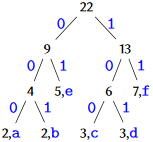
\includegraphics[scale=0.8]{../images/Baum.PNG}
				\begin{tabular}{c c c c c c c}
					\textbf{Häufigkeiten:}\\
					\hline
					x  &a&b&c&d&e&f\\
					\hline
					$N_x(w)$& 2& 2&3&3& 5& 7\\
					\hline
				\end{tabular}	
			}
		\end{itemize} 
		\pause
		\item Ablesen der Codes aus dem Baum (Pfadbeschriftungen)
	\end{enumerate}
	\only<4>{
		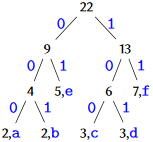
\includegraphics[scale=0.46]{../images/Baum.png}
		\hspace{0.4cm}
		\begin{tabular}{c c c c c c c}
			\textbf{Häufigkeiten:}\\
			\hline
			x &a&b&c&d&e&f\\
			\hline
			$N_x(w)$ & 2& 2&3&3& 5& 7\\
			
			\textbf{Codewörter:}\\
			\hline
			x &a&b&c&d&e&f\\
			\hline
			h(x)& 000& 001&100&101& 01& 11\\
			\hline
		\end{tabular}							
	}		
\end{frame}

\begin{frame}{Übung zu Huffman Codierung}
	\begin{taskblock}{Übung}
		Sei $A = \{$\texttt a, b, c, d, e, f, g, h$\}$\\
		\begin{itemize}
			\item Codiere das Wort \texttt{badcfehg} mit Hilfe der Huffman-Codierung \pause
			\item [$\rightarrow$]Mögliche Lösung: 001 100 010 011 101 000 111 110
			\pause
			\item Wie lauten die Codewörter, wenn für das Wort $w$ gilt: $N_a(w) = 1, N_b(w) = 2, N_c(w) = 2, N_d(w) =8, N_e(w) =16, N_f(w) =32, N_g(w) = 64, N_h(w) = 128$
			
		\end{itemize} \pause
		Mögliche Lösung:\\
		\begin{tabular}{|c|c c c c c c c c|}
			\hline
			x &a&b&c&d&e&f&g&h\\
			\hline
			h(x)& 0000000& 0000001&000001&00001& 0001&001& 01&1\\
			\hline
		\end{tabular}
	\end{taskblock}
\end{frame}	

	\begin{frame}
	\begin{itemize}
		\item Wie lang wäre das zweite Wort (\texttt{abbcccc} $\texttt{d}^{8}$...$\texttt{g}^{64}\texttt{h}^{128}$) mit dem ersten Code codiert? 
		\pause
		\item[$\rightarrow$] 741 Symbole. Also dreimal so lang wie das Original. \pause
		\item Wie lang wäre das zweite Wort mit dem zweiten Code codiert?\pause
		\item[$\rightarrow$] 501 Symbole. Also nur zweimal so lang wie das Original. \pause
		\item Was fällt euch auf?
	\end{itemize}
\end{frame}		

\begin{frame}{Wahr oder falsch?}
	Sei $h: A^* \rightarrow \mathbb{Z}_2$ eine Huffman-Codierung
	\begin{itemize}
		\item h ist ein $\varepsilon$-freier Homomorphismus \pause \textbf{Wahr!}\pause
		\item Häufigere Symbole werden mit langen Worten codiert, seltene mit kürzeren \pause \textbf{Falsch!}\pause
		\item Die Kompression ist am stärksten, wenn die Häufigkeiten aller Zeichen ungefähr gleich sind. \pause \textbf{Falsch!} \pause
		\item h ist präfixfrei \pause \textbf{Wahr!} \pause
		\item Es kann noch kürzere Codierungen geben \pause \textbf{Falsch!}
	\end{itemize}
\end{frame}

	
\begin{frame}{Huffman-Codierung}
	\begin{block}{Eigenschaften}
		Sei $A$ ein Alphabet und $w \in A$. Dann gilt für die Huffman-Codierung h:
		\begin{itemize}
			\item $h: A^* \rightarrow \mathbb{Z}_2$
			\item $h$ ist $\varepsilon$-freier Homomorphismus
			\item $h$ ist präfixfreier Homomorphismus
			\item Häufigere Symbole werden mit kurzen Worten codiert, seltene mit längeren
			\item Produziert kürzestmögliche Codierungen
		\end{itemize}
	\end{block}
\end{frame}

\begin{frame}{Block-Codierung mit Huffman}
	\begin{itemize}
		\pitem Wir betrachten nicht mehr einzelne Symbole, sondern Blöcke von fester Länge $b > 1$
		\pitem Blätter des Huffman-Baums sind jetzt \textit{Wörter der Länge b}
	\end{itemize}

	\vspace{.5cm}
	
	Beispiel an der Tafel: Codierung von $aab\cdot deg \cdot deg \cdot aab \cdot ole \cdot aab \cdot deg \cdot aab$.\p
	
	\vspace{.5cm}
	
	\p
	\begin{itemize}
		\pitem Alphabet $A =\{$\texttt{a,b,c,d} $\}$
		\pitem Text über $A$, der nur aus Teilwörtern der Länge 10 zusammengesetzt ist, in denen jeweils immer nur ein Symbol vorkommt
		%\item z.B. \texttt{aaaaaaaaaabbbbbbbbbbcccccccccc}...
		\pitem Angenommen $\texttt{a}^{10}$, ..., $\texttt{d}^{10}$ kommen alle gleich häufig vor. Wie lang ist dann die Huffman-Codierung? \pause
		\pitem[$\rightarrow$] Ein Fünftel, weil jeder Zehnerblock durch zwei Bits codiert wird
	\end{itemize}
	
\end{frame}


\begin{frame}
	
\includegraphics[width=\linewidth]{../images/thatsall.png}
\end{frame}

\end{document}
\def\tutdate{22.11.2018}
\def\tutTitle{Speicher, MIMA}

\documentclass[handout]{beamer}
\usepackage{../templates/beamerthemekitwide}
%\usepackage{enumitem}

\usepackage[utf8]{inputenc}
\usepackage[T1]{fontenc}
\usepackage[ngerman]{babel}
\usepackage{listings}
\usepackage{hyperref}
\usepackage{graphicx}

\usepackage{amsmath}
\usepackage{amsthm}
\usepackage{amssymb}
\usepackage{polynom}

%\usepackage{ifthen}
%\usepackage{adjustbox} % for \adjincludegraphics

%\usepackage{tikz}
\usepackage{listings}

%\usepackage[]{algorithm2e}

%\usepackage{colortbl}
\usepackage{verbatim}
%\usepackage{alltt}
%\usepackage{changes}

%\usepackage{pdfpages}
%\usepackage{tabularx}

%\usepackage{euler}


\newcommand{\markBlue}[1]{\textcolor{kit-blue100}{#1}}
\newcommand{\markGreen}[1]{\textcolor{kit-green100}{#1}}
\newcommand{\vertspace}{\vspace{.2cm}}

%\newcommand{\#}{\markBlue{#1}}

%\newcommand{\pitem}{\pause\item}
\newcommand{\p}{\pause}

% -- MATH MACROS
\newcommand{\thistheoremname}{}
\newcommand{\G}{\mathbb{Z}}
\newcommand{\B}{\mathbb{B}}
\newcommand{\R}{\mathbb{R}}
\newcommand{\N}{\mathbb{N}}
\newcommand{\Q}{\mathbb{Q}}
\newcommand{\C}{\mathbb{C}}
\newcommand{\Z}{\mathbb{Z}}
\newcommand{\F}{\mathbb{F}}
\newcommand{\mi}{\mathrm{i}}
\renewcommand{\epsilon}{\varepsilon}
\newcommand{\okalk}{\mathscr{O}}


\newenvironment<>{taskblock}[1]{%
	\setbeamercolor{block title}{fg=kit-orange15,bg=kit-orange100}
	\setbeamercolor{block body}{fg=black,bg=kit-orange30}%
	\begin{block}#2{#1}}{\end{block}}

\setbeamertemplate{enumerate items}[default]

% Aussagenlogik Symbole
\newcommand{\W}{w}
\renewcommand{\F}{f}

% Kodierung
\newcommand{\frepr}{\textbf{repr}}
\newcommand{\fRepr}{\textbf{Repr}}
\newcommand{\fZkpl}{\textbf{Zkpl}}
\newcommand{\fbin}{\textbf{bin}}
\newcommand{\fdiv}{\textbf{ div }}
\newcommand{\fmod}{\textbf{ mod }}

% Speicherabbild
\newenvironment{memory}{\begin{tabular}{r | l}Adresse&Wert\\\hline\hline}{\end{tabular}}
\newcommand{\memrow}[2]{#1 & #2 \\\hline}

% Praedikatenlogik
\newcommand{\objequiv}{\stackrel{\cdot}{=}}
\newcommand{\pval}{val_{D,I,\beta}}

% Neue Befehle
\newcommand{\ip}{\pause} % inline pause, für mitten im satz
\newcommand{\pitem}{\pause\item} % für aufzählungen
\newcommand{\bp}{\pause} % block pause, für zwischen blöcken
\title[Grundbegriffe der Informatik]{ICPC\\Gruppe 2}
\date{\tutdate}
\subtitle{\tutTitle}
\author{Elias Schaut, Dennis Kobert, Niklas Kniep, Lam Vo, Ilia Bozhinov}

\institute{}

\titleimage{bg}
%\titleimage{bg-advent}

%
\ifthenelse{\equal{\compiletype}{livebeamer}}
	{
		\def\livebeamermode{1}
	}{}

\ifthenelse{\equal{\compiletype}{print}}
	{
		\def\printmode{1}
	}{}

\setbeamercovered{invisible}

%\usepackage[citestyle=authoryear,bibstyle=numeric,hyperref,backend=biber]{biblatex}
%\addbibresource{templates/example.bib}
%\bibhang1em


\begin{document}

\selectlanguage{ngerman}

%title page
\begin{frame}
	\titlepage
\end{frame}

% Zur Anpassung: Dekommentiere folgende Zeilen, um weniger \pause zu haben
\renewcommand{\ip}{} % inline pause, für mitten im satz

% Dekommentiere folgende Zeilen, um Stil besser an deine Folien anzupassen
%\renewenvironment{taskblock}[1]{\textbf{Aufgabe: #1}\\}{}
%\renewcommand{\markBlue}[1]{\textbf{#1}}
%\renewcommand{\markGreen}[1]{\textbf{#1}}

\section{Hinweise}

\begin{frame} {Häufige Fehler}
\begin{itemize}
	\item Reguläre Ausdrücke:
	\item Nur $\{$, $\}$, (, ), $*$, $\cup$ und $\cdot$ dürfen verwendet werden
	\pitem $\{a\} \cdot \{b\} = \{ab\}$
	\pitem Unterschied zwischen $\{a\}* \cup \{b\}*$ und $\{a\}* \cdot \{b\}*$
	\pitem Keine äußeren Klammern
	\pitem Berechnungen mit Num, Repr haben keinen Rechenweg verlangt
	\pitem $|\epsilon| < 8$
\end{itemize}
\end{frame}

\section{Speicher}

\begin{frame}{Speicher}
	\begin{itemize}
		\pitem Ein \textbf{Bit} ist Zeichen aus $A = \{0, 1\}$
		\pitem Ein \textbf{Byte} ist ein Wort aus acht Bits
		\pitem Abkürzungen
		\begin{itemize}
			\pitem Für Bit: \texttt{bit}
			\pitem Für Byte: \texttt{B}
		\end{itemize}
	\end{itemize}
\end{frame}

\begin{frame}{Präfixe}
	\begin{center}
		\textbf{Dezimal}\\
		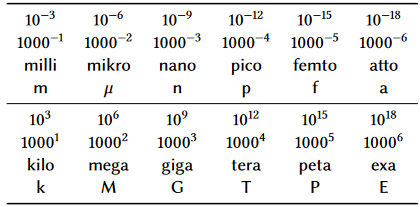
\includegraphics[scale=0.6]{../images/dezimal.png}\\ \pause
		\textbf{Binär}\\
		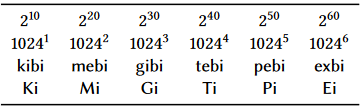
\includegraphics[scale=0.6]{../images/binaer.png}
	\end{center}
	
\end{frame}

\begin{frame}{Gesamtzustand eines Speichers}
	\p Zu jedem Zeitpunkt ist
	\begin{itemize}
		\pitem für jede \markBlue{Adresse} festgelegt, welcher \markBlue{Wert} dort ist
		\pitem beides meist Bitfolgen
	\end{itemize}
	\p Vorstellung: Tabelle mit zwei Spalten\\
	\begin{center}
		\begin{tabular}{|l l|}
			\hline
			\textbf{Adresse} & \textbf{Wert} \\
			\hline
			Adresse 1& Wert 1 \\
			Adresse 2 & Wert 2 \\
			Adresse 3 & Wert 3 \\
			...&...\\
			Adresse n & Wert n\\
			\hline
		\end{tabular}
	\end{center}
\end{frame}

\begin{frame}{Zustand eines Speichers -- formal}
	\p\begin{block}{Definition des Speicherzustandes}
		Sei $Adr$ die Menge aller Adressen und $Val$ die Menge aller Werte.\\
		Dann ist \\ \begin{center}
			$m: Adr \rightarrow Val$
		\end{center}
		der aktuelle Zustand des Speichers. Dabei ist $m(a)$ der aktuelle Wert an der Adresse $a$.
	\end{block}
\end{frame}


\begin{frame}{Lesen und Speichern}
	\pause
	\begin{block}{$Mem$}
		Menge aller möglichen Speicherzustände, also Menge aller Abbildungen von $Adr$ nach $Val$
		\begin{center}
			$Mem:= Val^{Adr}$
		\end{center}
	\end{block}
	\p Anmerkung: \p Für zwei Mengen $A$, $B$ gilt\p : $A^B := \{f: B \rightarrow A\}$.\p
	\begin{block}{$memread$}
		\begin{center}
			$memread: Mem \times Adr \rightarrow Val \text{ mit } (m, a) \mapsto m(a)$
		\end{center}
	\end{block}
	\pause
	\begin{block}{$memwrite$}
		$memwrite: Mem \times Adr \times Val \rightarrow Mem \text{ mit } (m, a,v) \mapsto m'$\\
		Für $m'$ wird folgendes gefordert:
		\begin{center}
			$m(a') :=\begin{cases} 
			v& \text{ falls } a' = a\\
			m(a') &\text{ falls } a' \neq a
			\end{cases} $ 
		\end{center}
	\end{block}
\end{frame}

\begin{frame}{Eigenschaften von $memread$ und $memwrite$}
	
	\begin{block}{Eigenschaften (``Invarianten'')}
		\begin{itemize}
			\pitem $memread(memwrite(m,a,v),a) = v$ \p (Also: An $a$ einen Wert $v$ zu schreiben und danach bei $a$ zu lesen gibt den Wert $v$ zurück \p $\Rightarrow$ Konsistente Datenhaltung)
			\pitem $memread(memwrite(m, a', v'),a) = memread(m,a)$ \p (Also: Auslesen einer Speicherstelle ist unabhängig davon, was vorher an eine andere Adresse geschrieben wurde \p $\Rightarrow$ Unabhängige Datenhaltung)
		\end{itemize}
	\end{block}

\end{frame}

\begin{frame}
	\textbf{Aufgaben}\\
	Aktueller Speicherzustand: \\
	\vspace{0.2cm}
	\begin{tabular}{|c| c|}
		\hline
		Adresse & Wert\\
		\hline
		00000& 01110\\
		00001& 00100\\
		00010& 00111\\
		00011& 00000\\
		...& ...\\
		\hline
	\end{tabular}\\
	\vspace{0.3cm}
	Was ist?
	\begin{itemize}
		\item $memread(memwrite(m, memread(m, 00011), 01010), 00000)$ \pause
		\item[$\rightarrow$] 01010
	\end{itemize}
	
\end{frame}

\section{MIMA}

\begin{frame}{Was ist die MIMA?}
	\begin{itemize}
		\pitem Theoretischer, idealisierter Prozessor
		\pitem Funktioniert wie ein echter Prozessor, ist aber simpler
		\pitem Nah an Technischer Informatik
	\end{itemize}

	\bp
	
	Grundaufbau:
	
	\begin{itemize}
		\pitem Adressen als $20bit$ Datenwort
		\pitem Speicherworte als $24bit$ Datenwort
		\pitem Maschinenbefehle als...
		\begin{itemize}
			\item $4bit$ Befehl und $20bit$ Adresse
			\item oder $8bit$ Befehl und unwichtigem Rest
		\end{itemize}
	\end{itemize}
\end{frame}

\begin{frame}{Aufbau der MIMA: Steuerwerk}
	\begin{center}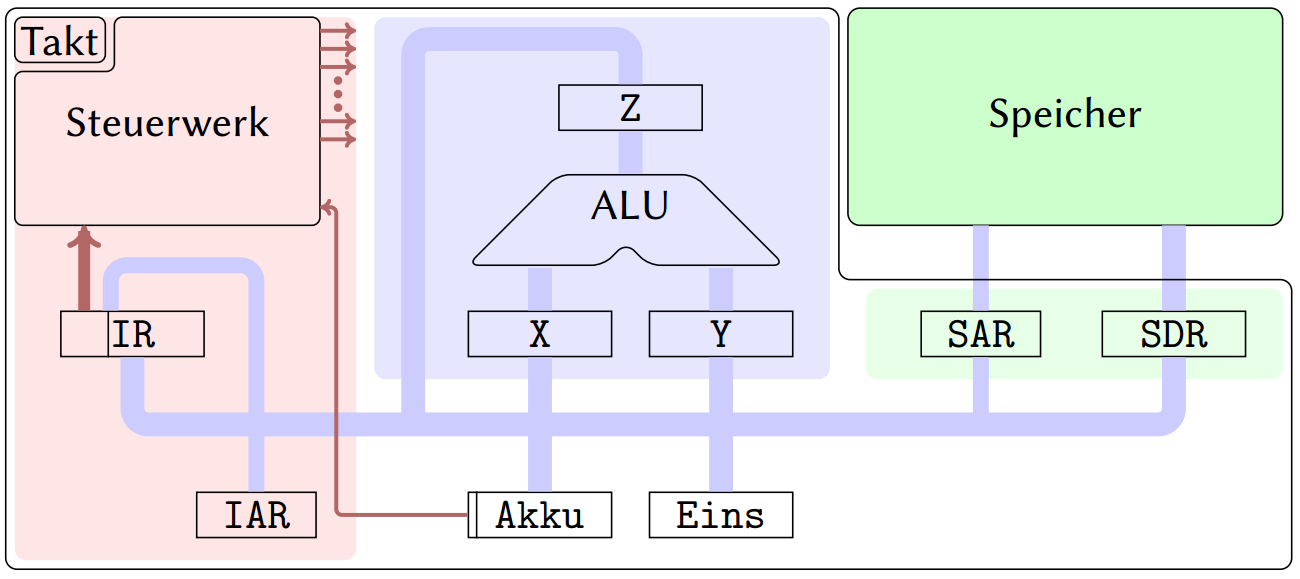
\includegraphics[width=.6\textwidth]{images/mima_aufbau.png}\end{center}
	
	\bp
	
	\textcolor{kit-red50}{\textbf{Steuerwerk}}
	
	\begin{columns}
		\begin{column}{0.5\textwidth}
			\begin{itemize}
				\pitem Instruction Register (IR) enthält den nächsten auszuführenden Befehl
				\pitem Instruction Adress Register (IAR) enthält die Adresse des nächsten Befehls
			\end{itemize}
		\end{column}
		
		\begin{column}{0.5\textwidth}
			\begin{itemize}
				\pitem Takt bestimmt die ``Tickrate'', also die Geschwindigkeit
				\pitem Steuerwerk interpretiert alle Befehle und führt sie aus
				\pitem Welche Befehle es gibt: Siehe später
			\end{itemize}
		\end{column}
	\end{columns}
	
\end{frame}


\begin{frame}{Aufbau der MIMA: Akku und Eins}
	\begin{center}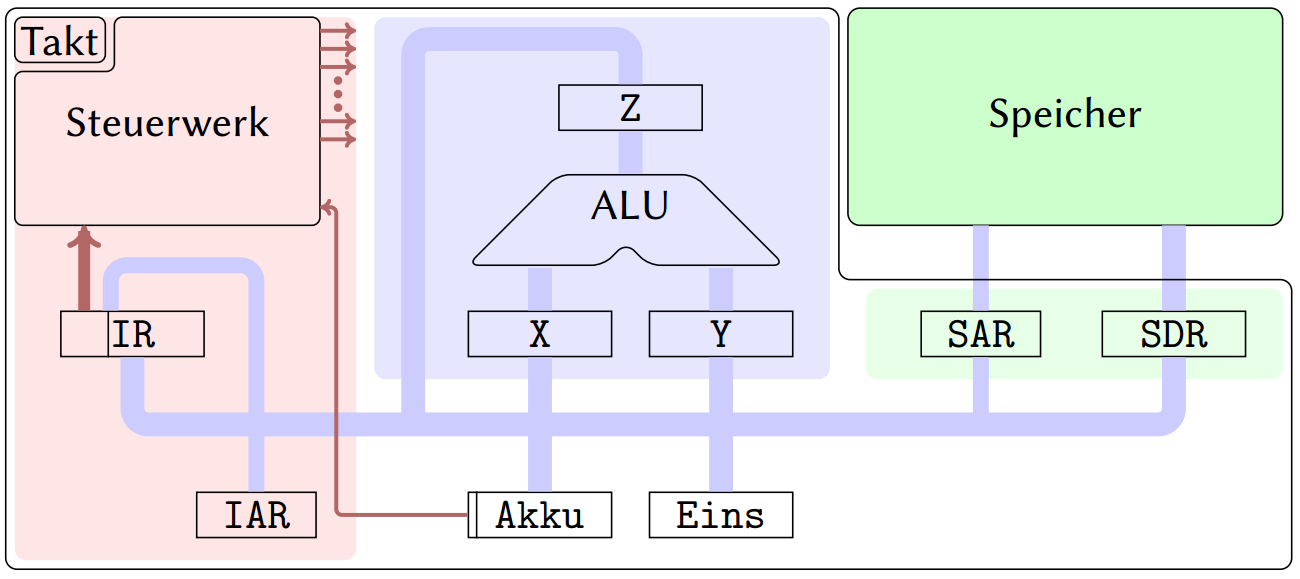
\includegraphics[width=.6\textwidth]{images/mima_aufbau.png}\end{center}
	
	\bp
	
	\textcolor{kit-orange50}{\textbf{Akku und Eins}}
	
	\begin{columns}
		\begin{column}{0.5\textwidth}
			\begin{itemize}
				\pitem Akku dient als Zwischenspeicher für Datenworte
				\pitem Hält maximal ein Wort
			\end{itemize}
		\end{column}
		
		\begin{column}{0.5\textwidth}
			\begin{itemize}
				\pitem Eins liefert die Konstante 1, hält also Strom
				\pitem z.B. erhöhen des IAR
			\end{itemize}
		\end{column}
	\end{columns}
	
\end{frame}


\begin{frame}{Aufbau der MIMA: ALU}
	\begin{center}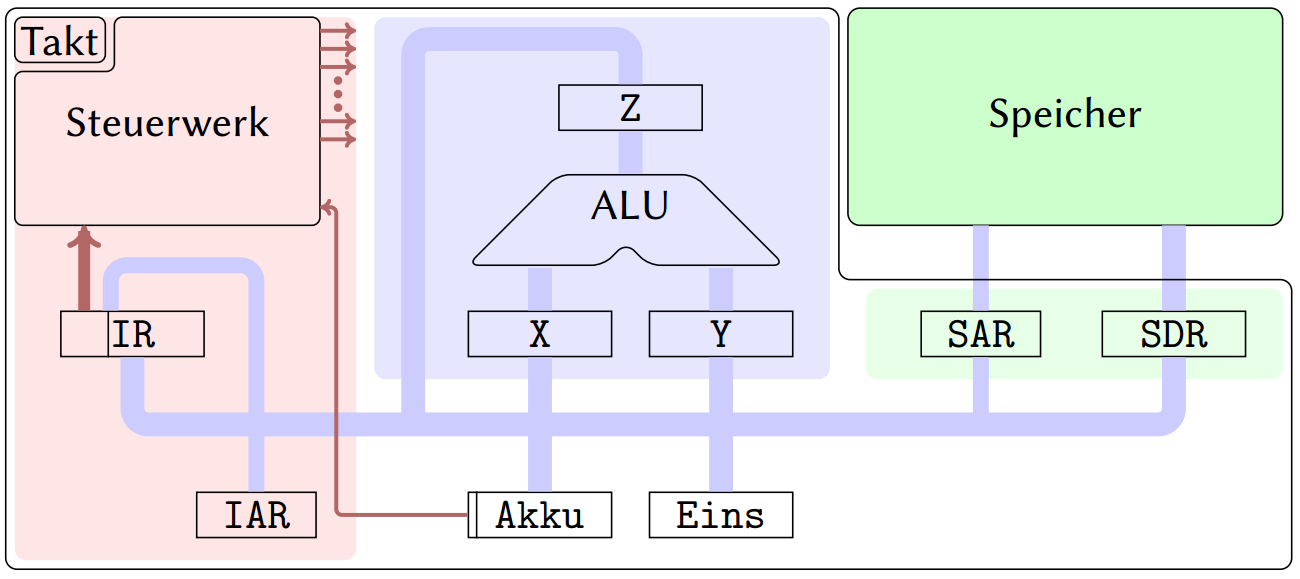
\includegraphics[width=.6\textwidth]{images/mima_aufbau.png}\end{center}
	
	\bp
	
	\textcolor{kit-blue50}{\textbf{Arithmetic Logic Unit (ALU) / Rechenwerk}}
	
	\begin{columns}
		\begin{column}{0.5\textwidth}
			\begin{itemize}
				\pitem Durchführt arithmetische Operationen
				\pitem $\fmod, \fdiv, +, -, ...$, bitweises OR/AND/...
			\end{itemize}
		\end{column}
		
		\begin{column}{0.5\textwidth}
			\begin{itemize}
				\pitem $X$ und $Y$ sind Eingaberegister
				\pitem $Z$ ist Ausgaberegister
			\end{itemize}
		\end{column}
	\end{columns}

\end{frame}


\begin{frame}{Aufbau der MIMA: ALU}
\begin{center}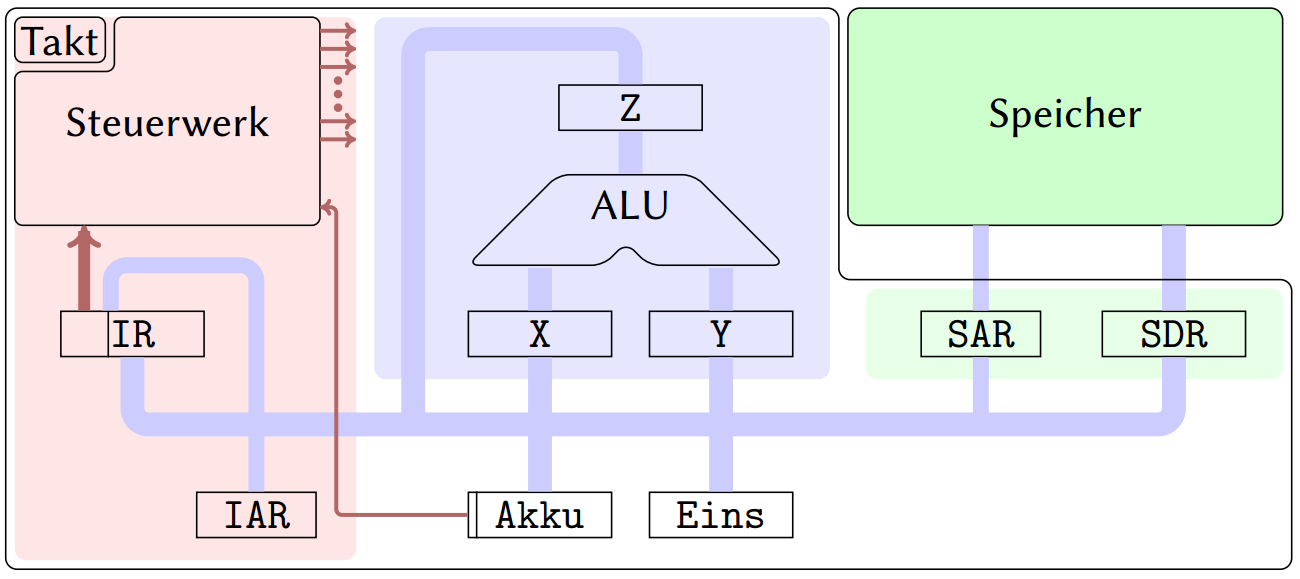
\includegraphics[width=.6\textwidth]{images/mima_aufbau.png}\end{center}

\bp

\textcolor{kit-green50}{\textbf{Speicher(werk)}}

Speicher selbst speichert Befehle und Daten. \ip Speicherwerk besteht aus:

\begin{columns}
	\begin{column}{0.5\textwidth}
		\begin{itemize}
			\pitem Speicheradressregister (SAR) ist die Adresse, bei der im Speicher gespeichert/gelesen werden soll
		\end{itemize}
	\end{column}
	
	\begin{column}{0.5\textwidth}
		\begin{itemize}
			\pitem Speicherdatenregister (SDR) Datum, das bei der Adresse gespeichert werden soll/ gelesen wurde.
		\end{itemize}
	\end{column}
\end{columns}

\end{frame}


\begin{frame}{Aufbau der MIMA: ALU}
\begin{center}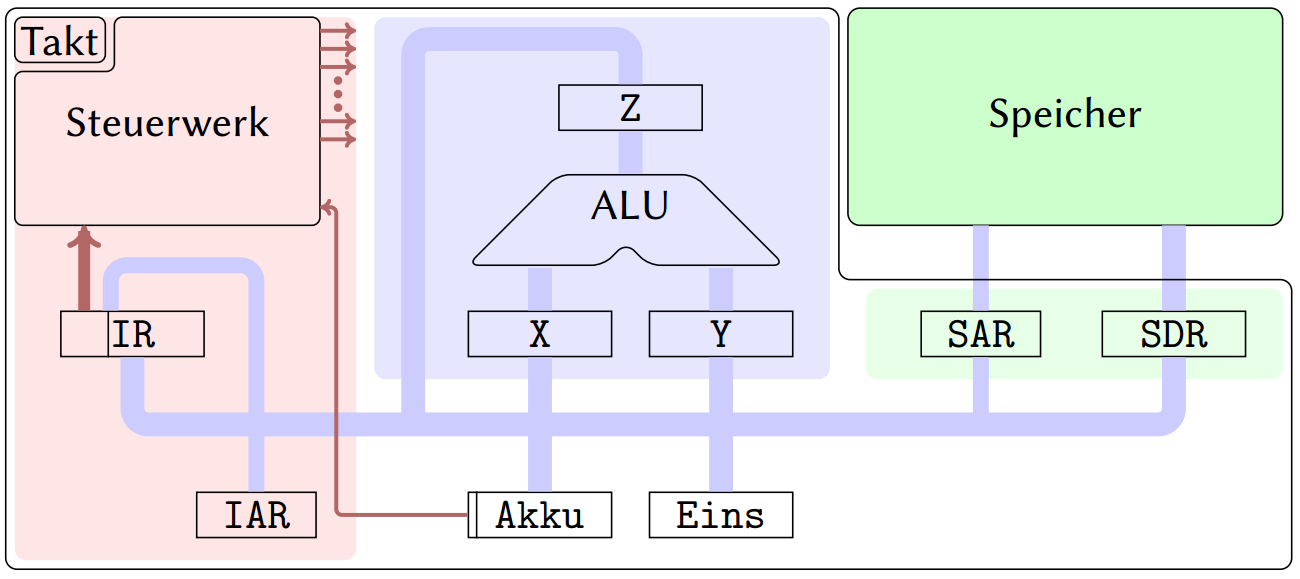
\includegraphics[width=.6\textwidth]{images/mima_aufbau.png}\end{center}

\bp

\textbf{Busse}

\begin{columns}
	\begin{column}{0.5\textwidth}
		\begin{itemize}
			\pitem ``Kabel'' zwischen den Verbindungen
			\pitem Ein kompletter Bus überträgt entweder $1$, $0$, oder nichts
		\end{itemize}
	\end{column}
	
	\begin{column}{0.5\textwidth}
		\begin{itemize}
			\pitem Kann nur eine einzige Information auf einmal übertragen
		\end{itemize}
	\end{column}
\end{columns}

\end{frame}

\begin{frame}{Konventionen zu MIMA Programmen}
	Um MIMA Programme und dazugehörige Definitionen verständlicher zu machen, vereinbaren wir folgende Konventionen:
	
	\bp
	
	\begin{itemize}
		\item Befehle (eigentlich Bitfolge) schreiben wir als Befehlname und Adresse
		\begin{itemize}
			\pitem $001000000000000000101010 \equiv STV$ $42$
		\end{itemize}
		\pitem $X \leftarrow Y \equiv $ ``Der Variable $X$ wird der Wert $Y$ zugewiesen''
		
	\end{itemize}
	
	
\end{frame}

\subsection{Maschinenbefehle}

% Folgende 3 Folien sollten nicht allzu ordentlich behandelt werden, mehr als vorzeitige Übersicht wieviele Befehle es gibt und als Referenz für die Tutanten für die Übungsaufgaben
\begin{frame}{MIMA Befehle}
	Eine MIMA-Maschine beherrscht folgende Maschinenbefehle:
	
	\vspace{.5cm}
	
	\begin{tabular}{r | l p{5cm} }
		Befehlssyntax & Formel & Bedeutung\\\hline\hline \ip
		$LDC$ $const$ & $Akku \leftarrow const$ & Lade eine Konstate $const$ in den Akku \\\hline \ip
		$LDV$ $adr$ & $Akku \leftarrow M(adr)$ & Lade einen Wert vom Speicher bei Adresse $adr$ in den Akku\\\hline\ip
		$STV$ $adr$ & $M(adr) \leftarrow Akku$ & Speichere den Wert aus dem Akku im Speicher bei Adresse $adr$\\\hline\ip
		$LDIV$ $adr$ & $Akku \leftarrow M(M(adr))$ & Lade einen Wert vom Speicher bei der Adresse, die bei $adr$ gespeichert ist, und lade den Wert in den Akku\\\hline\ip
		$STIV$ $adr$ & $M(M(adr)) \leftarrow Akku$ & Speichere den Wert im Akku bei der Adresse, die in $adr$ gespeichert ist.
	\end{tabular}
\end{frame}

\begin{frame}{MIMA Befehle (2)}
	Eine MIMA-Maschine beherrscht folgende Maschinenbefehle:
	
	\vspace{.5cm}
	
	\begin{tabular}{r | l p{3cm} }
		Befehlssyntax & Formel & Bedeutung\\\hline\hline \ip
		$ADD$ $adr$ & $Akku \leftarrow Akku + M(adr)$ & Addiere den Wert bei $adr$ zum Akku dazu.\\\hline\ip
		$``OP''$ $adr$ & $Akku ``OP'' M(adr)$ & Wende bitweise Operation auf Akku mit Wert bei $adr$ an. $Op \in \{AND, OR, XOR\}$.
	\end{tabular}
\end{frame}

\begin{frame}{MIMA Befehle (3)}
	Eine MIMA-Maschine beherrscht folgende Maschinenbefehle:
	
	\vspace{.5cm}
	
	\begin{tabular}{r | p{8cm} }
		Befehlssyntax & Bedeutung\\\hline\hline \ip
		$NOT$ & Bitweise Invertierung aller Bits des Akku-Datenwortes\\\hline\ip
		$RAR$ & Rotiere alle Akku-Bits eins nach rechts\\\hline\ip
		$EQL$ $adr$ & Setze Akku auf $11\cdots11$, falls Wert bei $adr$ gleich Akku-Wert, setze Akku auf $00\cdots00$ sonst.\\\hline\ip
		$JMP$ $adr$ & Springe zu Befehlsadresse $adr$\\\hline\ip
		$JMN$ $adr$ & Springe zu Befehlsadresse $adr$, falls Akku negativ (also erstes Bit $=1$), sonst fahre normal fort.
	\end{tabular}
\end{frame}

% Bei folgenden Folien eventuell den Speicher auf die Tafel abschreiben und das Programm Befehl für Befehl durchgehen

% Laden und Speichern
\begin{frame}{MIMA Befehle: Sichern und Laden}
	\begin{itemize}
		\pitem Befehle zum laden und Speichern in den Speicher
		\pitem LDV um Daten vom Speicher zu laden, STV um Daten in den Speicher zu schreiben
		\pitem LDC um eine Konstante zu laden
		\pitem Daten werden in einem Zwischenspeicher gelagert, der nur ein Datenwort hält\ip : Akku.
	\end{itemize}

	\bp

	Beispiele:
	
	\begin{itemize}
		\pitem $LDV$ $9$ lädt das Datum, das im Speicher bei Adresse $9$ liegt, in den Akku.
		\pitem $STV$ $9$ speichert das Datum, das im Akku liegt, in den Speicher an Adresse $9$.
		\pitem $LDC$ $4$ lädt die Zahl $4$ in den Akku (also kein Speicherzugriff).
	\end{itemize}
\end{frame}

\begin{frame}{MIMA Befehle: Sichern und Laden}
	\begin{tabular}{r | l p{5cm} }
		Befehlssyntax & Formel & Bedeutung\\\hline\hline 
		$LDC$ $const$ & $Akku \leftarrow const$ & Lade eine Konstate $const$ in den Akku \\\hline 
		$LDV$ $adr$ & $Akku \leftarrow M(adr)$ & Lade einen Wert vom Speicher bei Adresse $adr$ in den Akku\\\hline
		$STV$ $adr$ & $M(adr) \leftarrow Akku$ & Lade Speichere den Wert aus dem Akku im Speicher bei Adresse $adr$\\\hline
	\end{tabular}

	\bp 
	\vspace{.5cm}
	\markGreen{Beispielprogramm mit initialem Speicherabbild}
	\vspace{.2cm}
	
	\begin{columns}
		\begin{column}{0.25\textwidth}
			LDC 5 \\ STV $a_1$ \\ LDC 7 \\ STV $a_2$ \\ $\vdots$
		\end{column}
		\begin{column}{0.25\textwidth}
			 $\vdots$ \\ LDV $a_1$ \\ STV $a_3$ \\ HALT
		\end{column}
		
		\begin{column}{0.5\textwidth}
			\begin{memory}
				\memrow{$a_1$}{0}	
				\memrow{$a_2$}{0}
				\memrow{$a_3$}{0}
			\end{memory}
		\end{column}
	\end{columns}

	%TODO Ergebnis
\end{frame}

% Laden und Speichern (indirekt)
\begin{frame}{MIMA Befehle: Indirektes Sichern und Laden}
	\begin{tabular}{r | l p{5cm} }
		Befehlssyntax & Formel & Bedeutung\\\hline\hline 
		$LDIV$ $adr$ & $Akku \leftarrow M(M(adr))$ & Lade einen Wert vom Speicher bei der Adresse, die bei $adr$ gespeichert ist, und lade den Wert in den Akku\\\hline
		$STIV$ $adr$ & $M(M(adr)) \leftarrow Akku$ & Speichere den Wert im Akku bei der Adresse, die in $adr$ gespeichert ist.
	\end{tabular}
	
	\bp 
	\vspace{.5cm}
	\markGreen{Beispielprogramm mit initialem Speicherabbild}
	\vspace{.2cm}
	
	\begin{columns}
		\begin{column}{0.5\textwidth}
			LDIV 4 \\ STV 5 \\ LDIV 5 \\ STIV 4 \\ HALT
		\end{column}
		
		\begin{column}{0.5\textwidth}
			\begin{memory}
				\memrow{$4$}{$6$}	
				\memrow{$5$}{$0$}
				\memrow{$6$}{$7$}
				\memrow{$7$}{$2$}
			\end{memory}
		\end{column}
	\end{columns}
\end{frame}

% Arithmetische Operationen
\begin{frame}{MIMA Befehle: Eins plus Eins}
	\begin{itemize}
		\pitem Befehle zu arithmetischen Operationen
		\pitem Eine ALU-Operation, angewandt auf dem Wert des Akkus und dem Wert an gegebener Adresse
		
		\bp
		
		\item Beispiele:
		\begin{itemize}
			\pitem $ADD$ $4$ addiert den Wert im Akku mit dem Wert aus dem Speicher an Adresse $4$ und legt das Resultat im Akku ab\ip . Achtung: Addition nicht mit dem Wert $4$!
			\pitem $AND$ $3$ führt bitweise Verundung zwischen dem Wert im Akku und dem Wert aus dem Speicher an Adresse $4$ durch und legt das Resultat im Akku ab.
		\end{itemize}
	\end{itemize}
\end{frame}


\begin{frame}{MIMA Befehle: Eins plus Eins}
	\begin{tabular}{r | l p{5cm} }
		Befehlssyntax & Formel & Bedeutung\\\hline\hline 
		$ADD$ $adr$ & $Akku \leftarrow Akku + M(adr)$ & Addiere den Wert bei $adr$ zum Akku dazu.\\\hline
		$``OP''$ $adr$ & $Akku ``OP'' M(adr)$ & Wende bitweise Operation auf Akku mit Wert bei $adr$ an. $Op \in \{AND, OR, XOR\}$.
	\end{tabular}
	
	\bp 
	\vspace{.5cm}
	\markGreen{Beispielprogramm mit initialem Speicherabbild}
	\vspace{.2cm}
	
	\begin{columns}
		\begin{column}{0.5\textwidth}
			LDC 5 \\ ADD 3 \\ AND 4 \\ STV 5 \\ LDC 12 \\ XOR 5 \\ HALT
		\end{column}
		
		\begin{column}{0.5\textwidth}
			\begin{memory}
				\memrow{$3$}{$3$}	
				\memrow{$4$}{$8$}
				\memrow{$5$}{$17$}
			\end{memory}
		\end{column}
	\end{columns}
\end{frame}

% Logische Operationen
\begin{frame}{MIMA Befehle: Bits und Bytes }
	\begin{itemize}
		\pitem $NOT$ invertiert alle Bits des Datums im Akku. \ip Beispiel $NOT$ mit $5$ im Akku, angenommen der Akku speichert bis zu 8 bits\ip : $5_{10} = 00000101_2$, nach der Invertierung: $1111 1010_2$.
		
		\pitem $RAR$ rotiert alle Bits des Datums im Akku um eine Stelle nach rechts. \ip Beispiel mit $5$ im Akku: $00000\markBlue{101}_2$ wird zu $\markBlue{1}00000\markBlue{10}_2$.
		
		\pitem $EQL$ $adr$ vergleicht den Wert im Akku mit dem Wert bei $addr$.
		\begin{itemize}
			\pitem Setzt Akku $= 11\cdots 11$ falls Werte gleich sind.
			\pitem Setzt Akku $= 00\cdots 00$ falls Werte nicht gleich sind.
		\end{itemize}
	\end{itemize}
\end{frame}
	
\begin{frame}{MIMA Befehle: Bits und Bytes }
	\begin{tabular}{r | p{8cm} }
		Befehlssyntax & Bedeutung\\\hline\hline 
		$NOT$ & Bitweise Invertierung aller Bits des Akku-Datenwortes\\\hline
		$RAR$ & Rotiere alle Akku-Bits eins nach rechts\\\hline
		$EQL$ $adr$ & Setze Akku auf $11\cdots11$, falls Wert bei $adr$ gleich Akku-Wert, setze Akku auf $00\cdots00$ sonst.\\\hline
	\end{tabular}
	
	\bp 
	\vspace{.5cm}
	\markGreen{Beispielprogramm mit initialem Speicherabbild}
	\vspace{.2cm}
	
	\begin{columns}
		\begin{column}{0.25\textwidth}
			LDC 5 \\ NOT \\ RAR \\ NOT \\ RAR \\ $\vdots$
		\end{column}
		\begin{column}{0.25\textwidth}
			$\vdots$ \\ RAR \\ EQL 15 \\ EQL 0 \\ HALT
		\end{column}
		
		\begin{column}{0.5\textwidth}
		\end{column}
	\end{columns}
\end{frame}

% Programmstruktur Operationen
\begin{frame}{MIMA Befehle: Springen}
	\begin{itemize}
		\pitem Normalerweise wird die Instruktionsadresse nach jedem Befehl um eins erhöht
		\pitem Also Befehle werden von oben nach unten abgearbeitet
		\pitem Mit Sprüngen kann man die MIMA zwingen, zu definierten Befehlen zu springen und damit die Vorgehensreihenfolge zu beeinflussen
		
		\vspace{.3cm} \bp
		
		\item $JMP$ $adr$ führt als nächsten Befehl den an Adresse $adr$ aus.
		\pitem $JMN$ $adr$ führt als nächsten Befehl den an Adresse $adr$ aus, \markGreen{falls der Akku negativ ist}.
		\begin{itemize}
			\pitem Also wenn das erste Bit im Akku negativ ist.
			\pitem Wenn vorher ein $EQL$ erfolgreich verglichen hat, wird also gesprungen.
			\pitem Wenn der Akku positiv ist, werden die Befehle nach $JMN$ normal weiter abgearbeitet.
		\end{itemize}
	\end{itemize}
\end{frame}
	
\begin{frame}{MIMA Befehle: Springen}
	\begin{tabular}{r | p{8cm} }
		Befehlssyntax & Bedeutung\\\hline\hline 
		$EQL$ $adr$ & Setze Akku auf $11\cdots11$, falls Wert bei $adr$ gleich Akku-Wert, setze Akku auf $00\cdots00$ sonst.\\\hline
		$JMP$ $adr$ & Springe zu Befehlsadresse $adr$\\\hline
		$JMN$ $adr$ & Springe zu Befehlsadresse $adr$, falls Akku negativ (also erstes Bit $=1$), sonst fahre normal fort.
	\end{tabular}
	
	\bp 
	\vspace{.5cm}
	\markGreen{Beispielprogramm mit initialem Speicherabbild}
	\vspace{.0cm}
	
	\begin{columns}
		\begin{column}{0.25\textwidth}
			\begin{align*}
				& \text{LDC 5} \\
				a_1: \quad  & \text{JMN } a_2 \\
				& \text{EQL 1} \\
				& \text{JMN } a_1 \\
				%& NOT \\ % sollte nicht erreicht sein
				%a_2: \quad & \text{JMP } a_3\\
				%& NOT \\ % sollte nicht erreicht sein
				%a_3: \quad & HALT
				\vdots
			\end{align*}
		\end{column}
		\begin{column}{0.25\textwidth}
			\begin{align*}
				%& \text{LDC 5} \\
				%a_1: \quad  & \text{JMN } a_2 \\
				%& \text{EQL 1} \\
				%& \text{JMN } a_1 \\
				\vdots \\
				& NOT \\ % sollte nicht erreicht sein
				a_2: \quad & \text{JMP } a_3\\
				& NOT \\ % sollte nicht erreicht sein
				a_3: \quad & HALT
			\end{align*}
		\end{column}
	
		\begin{column}{0.5\textwidth}
			\begin{memory}
				\memrow{$1$}{$5$}	
			\end{memory}
		\end{column}
	\end{columns}
\end{frame}

\subsection{Aufgaben}

\begin{frame}{Aufgaben}
	\begin{taskblock}{MIMA-Programm schreiben}
		Schreibe ein MIMA-Programm:
		\begin{itemize}
			\item Eingabe: Adresse $a_1$ einer positiven Zahl $x$.
			\item Ausgabe: Speichert $3 \cdot x$ in $a_1$.
		\end{itemize}
	\end{taskblock}
	
	\bp \vspace{.5cm} Lösung:
	
	LDV $a_1$ \\ ADD $a_1$ \\ ADD $a_1$ \\ STV $a_1$ \\ HALT
\end{frame}

\begin{frame}{Aufgaben}
	\begin{taskblock}{MIMA-Programm schreiben}
		Schreibe ein MIMA-Programm:
		\begin{itemize}
			\item Eingabe: Adresse $a_1$ einer positiven Zahl $x$.
			\item Ausgabe: Speichert $x \fmod 2$ in $a_1$.
		\end{itemize}
	\end{taskblock}

	\bp \vspace{.5cm} Lösung:
	
	LDC 1 \quad // 000000000000000000000001 \\ AND $a_1$ \\ STV $a_1$ \\ HALT
\end{frame}

\begin{frame}{Aufgaben}
	\begin{taskblock}{MIMA-Programm schreiben}
		Schreibe ein MIMA-Programm:
		\begin{itemize}
			\item Eingabe: Adresse $a_1$ einer positiven Zahl $x$.
			\item Ausgabe: Speichert $x \fdiv 2$ in $a_1$.
		\end{itemize}
	\end{taskblock}
	
	\bp \vspace{.5cm} Lösung:
	
	LDC 1 \\ NOT \\ AND $a_1$ \quad // Setze ``rechtestes'' Bit auf 0 \\ RAR \\ STV $a_1$ \\ HALT
\end{frame}


\begin{frame}
	
\includegraphics[width=\linewidth]{../images/thatsall.png}
\end{frame}


\end{document}
\def\tutdate{29.11.2018}

\documentclass[handout]{beamer}
\usepackage{../templates/beamerthemekitwide}
%\usepackage{enumitem}

\usepackage[utf8]{inputenc}
\usepackage[T1]{fontenc}
\usepackage[ngerman]{babel}
\usepackage{listings}
\usepackage{hyperref}
\usepackage{graphicx}

\usepackage{amsmath}
\usepackage{amsthm}
\usepackage{amssymb}
\usepackage{polynom}

%\usepackage{ifthen}
%\usepackage{adjustbox} % for \adjincludegraphics

%\usepackage{tikz}
\usepackage{listings}

%\usepackage[]{algorithm2e}

%\usepackage{colortbl}
\usepackage{verbatim}
%\usepackage{alltt}
%\usepackage{changes}

%\usepackage{pdfpages}
%\usepackage{tabularx}

%\usepackage{euler}


\newcommand{\markBlue}[1]{\textcolor{kit-blue100}{#1}}
\newcommand{\markGreen}[1]{\textcolor{kit-green100}{#1}}
\newcommand{\vertspace}{\vspace{.2cm}}

%\newcommand{\#}{\markBlue{#1}}

%\newcommand{\pitem}{\pause\item}
\newcommand{\p}{\pause}

% -- MATH MACROS
\newcommand{\thistheoremname}{}
\newcommand{\G}{\mathbb{Z}}
\newcommand{\B}{\mathbb{B}}
\newcommand{\R}{\mathbb{R}}
\newcommand{\N}{\mathbb{N}}
\newcommand{\Q}{\mathbb{Q}}
\newcommand{\C}{\mathbb{C}}
\newcommand{\Z}{\mathbb{Z}}
\newcommand{\F}{\mathbb{F}}
\newcommand{\mi}{\mathrm{i}}
\renewcommand{\epsilon}{\varepsilon}
\newcommand{\okalk}{\mathscr{O}}


\newenvironment<>{taskblock}[1]{%
	\setbeamercolor{block title}{fg=kit-orange15,bg=kit-orange100}
	\setbeamercolor{block body}{fg=black,bg=kit-orange30}%
	\begin{block}#2{#1}}{\end{block}}

\setbeamertemplate{enumerate items}[default]

% Aussagenlogik Symbole
\newcommand{\W}{w}
\renewcommand{\F}{f}

% Kodierung
\newcommand{\frepr}{\textbf{repr}}
\newcommand{\fRepr}{\textbf{Repr}}
\newcommand{\fZkpl}{\textbf{Zkpl}}
\newcommand{\fbin}{\textbf{bin}}
\newcommand{\fdiv}{\textbf{ div }}
\newcommand{\fmod}{\textbf{ mod }}

% Speicherabbild
\newenvironment{memory}{\begin{tabular}{r | l}Adresse&Wert\\\hline\hline}{\end{tabular}}
\newcommand{\memrow}[2]{#1 & #2 \\\hline}

% Praedikatenlogik
\newcommand{\objequiv}{\stackrel{\cdot}{=}}
\newcommand{\pval}{val_{D,I,\beta}}

% Neue Befehle
\newcommand{\ip}{\pause} % inline pause, für mitten im satz
\newcommand{\pitem}{\pause\item} % für aufzählungen
\newcommand{\bp}{\pause} % block pause, für zwischen blöcken
\title[Grundbegriffe der Informatik]{ICPC\\Gruppe 2}
\date{\tutdate}
\subtitle{\tutTitle}
\author{Elias Schaut, Dennis Kobert, Niklas Kniep, Lam Vo, Ilia Bozhinov}

\institute{}

\titleimage{bg}
%\titleimage{bg-advent}

%
\ifthenelse{\equal{\compiletype}{livebeamer}}
	{
		\def\livebeamermode{1}
	}{}

\ifthenelse{\equal{\compiletype}{print}}
	{
		\def\printmode{1}
	}{}

\setbeamercovered{invisible}

%\usepackage[citestyle=authoryear,bibstyle=numeric,hyperref,backend=biber]{biblatex}
%\addbibresource{templates/example.bib}
%\bibhang1em


\def\tutTitle{Kontextfreie Grammatiken, Relationen}
\begin{document}
	
	\selectlanguage{ngerman}
	
%title page
\begin{frame}
	\titlepage
\end{frame}

\section{Hinweise}

\begin{frame}
Erinnerung: Anmeldung für Klausur und Übungsschein im Campus System nicht vergessen!
\end{frame}

\begin{frame} {Häufige Fehler}
\begin{itemize}
	\item $w \in \{0, 1\}^*$
	\item nicht $w \geq 0$, sondern $Num_2 (w) \geq 0$ oder $w(0)=0$
	\pitem $f:A \rightarrow A^*$ induziert den Homomorphismus $f^{**}:A^* \rightarrow A^*$, ist aber selbst keiner
	\pitem $h:A^* \rightarrow A^*$ mit $\forall w \in A^*: h(w) = 0$ ist kein Homomorphismus. Warum nicht?
\end{itemize}
\end{frame}

\section{Kontextfreie Grammatiken}
\begin{frame}{Kontextfreie Grammatiken}
	Zur Rekapitulation...
	
	\begin{itemize}
		\pitem Was ist ein Alphabet, was eine formale Sprache?
		\pitem Was kennen wir für Operationen auf formalen Sprachen?
	\end{itemize}

	\bp 
	
	Betrachte $L := \{a^nba^n : n \in \N \}$. \ip Wie kann man diese Sprache darstellen?
\end{frame}

\begin{frame}{Kontextfreie Grammatiken}
	\begin{block}{Kontextfreie Grammatik}
		Ein Tupel G = (N, T, S, P) mit
		\begin{itemize}
			\item $N$ Alphabet (Nichtterminalsymbole)
			\item $T$ Alphabet mit $N \cap T = \emptyset$ (Terminalsymbole)
			\item $S \in N$ (Startsymbol)
			\item $P \subseteq N \times (N \cup T)^* \text{ mit } |P| \in \mathbb{N}_0$
		\end{itemize}
	\end{block}

	\begin{itemize}
		\pitem Was ist $N \times (N \cup T)^*$? Bei $T := \{a,b,c\}, N = \{S, A, B\}$\ip : $N \times (N \cup T)^* = \{(S, abSAcB), (A, SSS), (B, BSabc), ...\}$.
		\pitem Andere Schreibweise: $P : N \rightarrow (N \cup T)^*$.
		\pitem Für $(X, w) \in P$ schreibt man $X \rightarrow w$
		\pitem Statt $\{X\rightarrow w_1, X \rightarrow w_2 \}$ schreibt man auch $\{X \rightarrow w_1 | w_2\}$
	\end{itemize}
	
\end{frame}

\begin{frame}{Ableitungsschritt}
	Erinnerung: $N = Nichtterminalsymbole$, $T = Terminalsymbole$. \pause
	
	\begin{block}{Ableitungsschritt}
		$v \in (N \cup T)^*$ ist in einem Schritt aus $u \in (N \cup T)^*$ ableitbar , wenn 
		\begin{itemize}
			\pitem $u = w_1 X w_2 \text{ und } v = w_1 w_X w_2 \text{ für } w_1, w_2 \in (N \cup T)^* $
			\pitem und $X \rightarrow w_X$ in $P$
		\end{itemize}
	\end{block}

	\bp\markBlue{Notation}\\
	$u\Rightarrow v$\\
	\bp\markBlue{Beispiel}\\
	$G:= (\{S,B\}, \{a,b\}, S, \{S \rightarrow aBa|aSa, B \rightarrow b\})$
	
	\begin{itemize}
		\pitem $S \ip\Rightarrow aSa \ip\Rightarrow aaSaa \ip\Rightarrow aaaBaaa \ip\Rightarrow aaabaaa$. \ip Fertig.
		\pitem $aaaSaaa \not\Rightarrow aaaabaaaa$! 
		\pitem ``$\Rightarrow$'' heißt \markGreen{eine} Ableitung!
	\end{itemize}
\end{frame}

\begin{frame}{Ableitungsfolge}
	\begin{block}{Ableitungsfolge}
	    Wir definieren $\Rightarrow^i$ für $i \in \mathbb{N}_0$ folgendermaßen:\\\vspace{.3cm}
		\bp Für $u,v \in (N \cup T)^*$ gelte:
		\begin{itemize}
			\item $u \Rightarrow^0 v$ genau dann, wenn $u = v$ gilt.
			\item $u \Rightarrow^{i+1} v$ genau dann, wenn ein $w \in (N \cup T)^* $ existiert, für das $u \Rightarrow w \Rightarrow^i v$ gilt.
			Für $u \Rightarrow^i v$ sagt man \markGreen{``v ist aus $u$ in $i$ Schritten ableitbar.''}
		\end{itemize}
	\end{block}

	\bp

	\textbf{Beispiel}\\
	$G:= (\{S,B\}, \{a,b\}, S, \{S \rightarrow aBa|aSa, B \rightarrow b\})$\\
	\ip Dann gilt $aaaSaaa \Rightarrow^0 aaaSaaa$ \ip \\
	und $aaaSaaa \Rightarrow^2 aaaabaaaa$
\end{frame}

\begin{frame}
	\begin{block}{Ableitbarkeit}
		Für $u,v \in (N \cup T)^*$ gelte $u \Rightarrow^* v$ genau dann, wenn ein $i \in \mathbb{N}_0$ existiert , mit $u \Rightarrow^i v$. Man sagt dann \markGreen{``v ist aus u ableitbar''}.
	\end{block}\bp
	\textbf{Beispiel}\\
	$G:= (\{S,B\}, \{a,b\}, S, \{S \rightarrow aBa|aSa, B \rightarrow b\})$\\
	\ip Dann gilt $S \Rightarrow^* aaaSaaa$ \ip \\
	und $aSa \Rightarrow^* aaaabaaaa$ \ip \\
	aber $aSa \not\Rightarrow abba$.
\end{frame}

\begin{frame}{Ableitungsbaum}
	\begin{columns}
		\begin{column}{0.5\textwidth}
			\begin{itemize}
				\item Startsymbol ist Wurzel
				\item Nichtterminale sind innere Knoten
				\item Für $X \Rightarrow w $ sind die Zeichen von $w$ die Kinder von X
				\item Terminale sind die Blätter
			\end{itemize}
		\end{column}
		
		\begin{column}{0.5\textwidth}\bp
			\textbf{Beispiel}\\
			$G:= (\{S,B\}, \{a,b\}, S, \{S \rightarrow aBa|aSa, B \rightarrow b\})$\bp\\
			Dann gilt $S \Rightarrow^* aaabaaa$\\
			\center 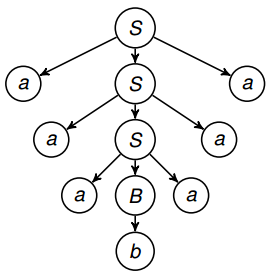
\includegraphics[scale=0.7]{images/Ableitungsbaum.png}
		\end{column}
	\end{columns}
	
\end{frame}

\begin{frame}{Übung zu Kontextfreien Grammatiken}
	\begin{taskblock}{Übung}
		Gegeben ist die Kontextfreie Grammatik (N, T, S, P) mit:
		
		\begin{itemize}
			\item Nichtterminalsymbolen $N := \{A, B, S\}$.
			\item Terminalsymbolen $T := \{a, b, c\}$
			\item Startsymbol $S$
			\item Produktionen $P := \{S \rightarrow aaS | bbS | SAS | \epsilon, A \rightarrow cB , B \rightarrow a | b| c | \epsilon\}$.
		\end{itemize}
	
		\bp
	
		Aufgabe: Welche der folgenden Wörter sind ableitbar? Konstruiere den Ableitungsbaum und zeige, wie sie abgeleitet werden.
		
		\begin{itemize}
			\item $ccbbcbbbbcbbaaaa$? %ja
			\item $aabbaabbaabb$? %ja
			\item $c$?
		\end{itemize}
	\end{taskblock}
\end{frame}

\begin{frame}{Formale Sprachen erzeugen}
	\begin{block}{Erzeugte Sprache}
		Sei $G = (N, T, S, P)$ eine kontextfreie Grammatik. Dann nennen wir $L(G) := \{w \in T^*| S \Rightarrow^* w\}$ die von G erzeugte Sprache.
	\end{block}

	\bp
	
	\begin{block}{Kontextfreie Sprache}
		Eine formale Sprache $L$ heißt genau dann kontextfrei, wenn eine kontextfreie Grammatik $G$ existiert, mit $L(G) = L$.
	\end{block}

	\bp

	$G:= (\{S,B\}, \{a,b\}, S, \{S \rightarrow aBa|aSa, B \rightarrow b\})$\\\vspace{.3cm}
	\ip Dann ist $L(G) = \{a^nba^n|n \in \mathbb{N_+}\}$
\end{frame}

\begin{frame}{Verständnisfragen}
	\begin{itemize}
		\item $G = (\{X\}, \{a,b\}, X, \{X \rightarrow \varepsilon| aX| bX\})$
		\begin{itemize}
			\item Welche Wörter lassen sich in genau drei Schritten ableiten?
			\pause		 		
			\item[$\rightarrow$] $\{aa, ab, ba, bb\}$
			\pause
			\item Was ist $L(G)$?
			\pause		 		
			\item[$\rightarrow$] $L(G) = \{a,b\}^*$
		\end{itemize}
		\pause
		\item Gibt es auch eine Grammatik $G$ mit $L(G) = \{\}$?
		\pause
		\item[$\rightarrow$] $G_1 := (\{X\}, \{a,b\}, X, \{X\rightarrow X\})$ oder $G_2 := (\{X\}, \{a,b\}, X, \{\})$
		\pause
		\item Wahr oder falsch? Wenn $w_1 \Rightarrow w_2$ gilt, dann gilt auch $w_1 \rightarrow w_2$
		\pause
		\item Was ist der Unterschied von $\Rightarrow$ und $\Rightarrow^*$ ?
	\end{itemize}
\end{frame}

\begin{frame}
	\begin{taskblock}{Aufgaben zu kontextfreien Grammatiken}
		\begin{itemize}
			\item Sei $L_1 := \{wbaaw'|w, w' \in \{a,b\}^*\}$. Konstruiere eine Grammatik $G_1$ mit $L(G_1) = L_1$.
			\pause
			\item[$\rightarrow$] $G_1 := (\{X, Y\}, \{a,b\}, X, \{X \rightarrow YbaaY, Y \rightarrow aY|bY|\varepsilon\})$.
			\pause
			\item  Welche Sprache erzeugt $ G_2 = (\{S, X, Y\}, \{a,b\}, S, P_2)$  mit $P_2 = \{S \rightarrow X|Y, X \rightarrow aaXb|aab, Y \rightarrow aYbb|abb\}$?
			\pause			
			\item[$\rightarrow$] $L(G_2) = \{a^{2k}b^{k} | k \in \mathbb{N}_+\} \cup \{a^kb^{2k}| k \in \mathbb{N}_+\}$
			%\pause
			%\item Sei $L_3 := \{w \in \{a,b\}^*| \forall \text{ Präfixe } v \text{ von } w : |N_a(v) - N_b(v)| \leq 1 \}$. Konstruiere eine Grammatik $G_3$ mit $L(G_3) = L_3$
			%\pause
			%\item[$\rightarrow$] $G_3 = (\{X\}, \{a,b\}, X, \{X\rightarrow abX|baX|a|b|\varepsilon\})$
		\end{itemize}
	\end{taskblock}	
\end{frame}

\begin{frame}{Beispiel zu kontextfreien Grammatiken}
	$G= (\{X\}, \{\textcolor{blue}{(}, \textcolor{blue}{)}\}, X, \{X \rightarrow XX|\textcolor{blue}{(} X \textcolor{blue}{)}| \varepsilon\} )$
	\begin{itemize}
		\item Welche Wörter sind ableitbar?
		\pause
		\item[$\rightarrow$] ``wohlgeformte Klammerausdrücke''
		\pause
		\item Welche Eigenschaften besitzen diese Wörter?
		\pause
		\item[$\rightarrow$]$N_{\textcolor{blue}{(}}(w) = N_{\textcolor{blue}{)}}(w)$ \pause Ist diese Eigenschaft hinreichend?
		\pause
		\item[$\rightarrow$]Nein, es muss gelten: Für alle Präfixe $v$ von $w$ gilt $ N_{\textcolor{blue}{(}}(v) \geq N_{\textcolor{blue}{)}}(v)$
		\pause
		\item Andere Grammatik möglich, die alle wohlgeformten Klammerausdrücke erzeugt?
		\pause
		\item[$\rightarrow$]  $G= (\{X\}, \{\textcolor{blue}{(}, \textcolor{blue}{)}\}, X, \{X \rightarrow \textcolor{blue}{(} X \textcolor{blue}{)}X| \varepsilon\} )$
	\end{itemize}
\end{frame}

\begin{frame}{Grenze kontextfreier Grammatiken}
	Es gibt auch Sprachen, die wir nicht mit einer kontextfreien Grammatik erzeugen können!
	
	\vspace{.3cm} \bp
	Beispiel aus der Vorlesung:\\
	$L_{vv} = \{vcv| v \in \{a,b\}^*\} \subseteq \{a, b, c\}^*$
\end{frame}


\section{Relationen vol. 2}
\begin{frame}{Relationen}
	\pause
	\begin{block}{Erinnerung Relationen}
		Es seien A und B Mengen. Eine Teilmenge $R \subseteq A \times B$ heißt Relation.
	\end{block}
\end{frame}

\begin{frame}	
	\begin{block}{Definition Produkt von Relationen}
		Es seinen $A, B \text{ und  } C$ Mengen und $R \subseteq A \times B, S \subseteq B \times C$ Relationen. Dann ist \\$S \circ R := \{(a,c) \in A \times C | \text{ } \exists b \in B \text{ mit } (a,b) \in R \land (b,c) \in S\}$ \\
		das Produkt der Relationen $R$ und $S$.
	\end{block}
	\bp\textbf{Bemerkung}\\
	\ip $S \circ R$ ist eine Relation auf $A$ und $C$\ip , bildet also von $A$ nach $C$ ab.
	\bp\begin{block}{Assoziativität des Produktes}
		Es seien $ A, B, C$ und $D$ Mengen und $R \subseteq A \times B, S \subseteq B \times C$ sowie $T \subseteq C \times D$ Relationen. 
		Dann gilt\ip \\
		$(T \circ S) \circ R = T \circ (S \circ R)$.
	\end{block}
\end{frame}

\begin{frame}
	\begin{block}{Homogene Relation}
		Es seien A und B Mengen und $R \subseteq A \times B$ eine Relation. $R$ heißt homogen, wenn $A=B$ und heterogen, wenn $A \neq B $ gilt.
	\end{block}
	
	\bp\begin{block}{Identität}
		Sei $M$ eine Menge. $I_M := \{(x,x)| x \in M\}$		
	\end{block}

	\bp\begin{block}{Potenz von Relationen}
		Sei $M$ eine Menge und $R \subseteq M  \times M$ eine homogene Relation. \ip Dann definieren wir $R^i$ für $i \in \mathbb{N}_0$ folgendermaßen: 
		\begin{itemize}
			\pitem $R^0 := I_M$
			\pitem Für alle $i \in \mathbb{N}_0: R^{i+1} := R^i \circ R$
		\end{itemize}
	
		\ip Also $R^4 = R \circ R \circ R \circ R$.
	\end{block}
\end{frame}

\begin{frame}{Reflexitivität}
	\bp\begin{block}{Satz über das neutrale Element}
		Es seien $A$ und $B$ Mengen und $R \subseteq A \times B$ eine Relation. Dann gilt: $R \circ I_B = R = I_A \circ R$.
	\end{block}
	
	\bp\begin{block}{Reflexivität}
		Sei M eine Menge und $R \subseteq M \times M$ eine homogene Relation. Wenn für alle $x \in M: (x,x) \in R$, nennt man $R$ reflexiv.
		
		\ip Also jedes Element der Definitionsmenge der Relation wird auf sich selbst abgebildet (und vielleicht auch auf andere Elemente abgebildet).
	\end{block}
	
	\bp\begin{block}{Lemma}
		Sei $M$ eine Menge und $R \subseteq M \times M$ eine homogene Relation. $R$ ist genau dann reflexiv, wenn $I_M \subseteq R$ gilt.
	\end{block}
\end{frame}

\begin{frame}{Transitivität}
	\bp\begin{block}{Transitivität}
		Sei $M$ eine Menge und $R \subseteq M \times M$ eine homogene Relation. \\ \ip R heißt transitiv, wenn: \ip\\ $\forall x, y, z \in M: (x,y) \in R \land (y, z) \in R \rightarrow (x,z) \in R$
	\end{block}
	
	\bp\begin{block}{Lemma}
		Sei $M$ eine Menge und $R \subseteq M \times M$ eine homogene Relation. $R$ ist genau dann transitiv, wenn $R \circ R \subseteq R$.
	\end{block}
\end{frame}

\begin{frame}
	\textbf{Aufgaben}\\
	Sei $M := \{1, 2, 3 \}$.
	\begin{itemize}
		\item Ist $R:= \{(1,1), (1,2), (2,3)\}$ transitiv? \pause Nein!
		\pause
		\item Ist $R$ reflexiv? \pause Nein!
		\pause
		\item Wie müsste R aussehen, um transitiv zu sein?
		\pause
		\item Ist $S:= \{(1,1), (1,2), (1,3), (2,2), (2,3)\}$ reflexiv? \pause Nein!
		\pause
		\item Ist $S$ transitiv? \pause \hspace{0.3cm} Ja!
		\item Wie müsste S aussehen, um reflexiv zu sein?
	\end{itemize}
\end{frame}

\begin{frame}{Reflexiv-transitive Hülle}
	\bp\begin{block}{Definition}
		Sei M eine Menge und $R \subseteq M \times M$ eine homogene Relation. \\Dann nennt man $R^* := \bigcup\limits_{i \in \mathbb{N}_0} R^i$ die reflexiv-transitive Hülle von R.
	\end{block}
	\bp\begin{block}{Satz}
		\begin{itemize}
			\item $R^*$ ist reflexiv
			\item $R^*$ ist transitiv
			\item $R^*$ ist die kleinste Relation, die reflexiv und transitiv ist und $R \subseteq R^*$ erfüllt.
		\end{itemize}
	\end{block}
	\bp\textbf{Bemerkung}\\
	\begin{itemize}
		\item Sei M eine Menge und $R\subseteq M \times M$ eine homogene, reflexive und transitive Relation. Dann gilt $R^* = R$.
	\end{itemize}
	
\end{frame}
\begin{frame}
	\textbf{Aufgaben}\\
	\begin{itemize}
		\item Sei $M = \{1, 2, 3\}$ und $R := \{(1,1), (1,2), (2,3)\}$ Was ist $R^*$?
		\pause
		\item[$\rightarrow$] $R^* = \{(1,1), (1,2), (1,3), (2,2), (2,3), (3,3)\}$ 
		\pause
		\item Sei $M$ eine Menge und $R \subseteq M \times M$ eine homogene Relation. Was ist $(R^*)^*$ ?
		\pause
		\item[$\rightarrow$]  $(R^*)^* = R^*$
		\pause
		\item $M := \{1,2,3,4\} \text{ und } R := \{(1,2), (2,3), (3,4), (4,1)\} \subseteq M \times M$. Ist R reflexiv? Ist R transitiv? \pause \hspace{0.3cm} Nein und nein!
	\end{itemize}
\end{frame}

\begin{frame}
	Die Relationen $R$ und $S$ über $\mathbb{N}_0$ seien gegeben durch:
	\begin{itemize}
		\item Für alle $a, b \in \mathbb{N}_0: aRb \Leftrightarrow a|b$ ($a$ ist Teiler von $b$)
		\item Für alle $a, b \in \mathbb{N}_0: aSb \Leftrightarrow ggT(a,b) = 1$ 
	\end{itemize}
	Prüfe auf Reflexivität und Transitivität!
	\pause
	\begin{itemize}
		\item[$\rightarrow$] R ist transitiv, aber nicht reflexiv.
		\pause
		\item[$\rightarrow$] S ist reflexiv, aber nicht transitiv.
	\end{itemize}
\end{frame}


\begin{frame}
	
\includegraphics[width=\linewidth]{../images/thatsall.png}
\end{frame}


\end{document}
\def\tutdate{09.12.2019}

\documentclass[]{beamer}
\usepackage{../templates/beamerthemekit}

\usepackage[utf8]{inputenc}
\usepackage[T1]{fontenc}
\usepackage[ngerman]{babel}
\usepackage{listings}
\usepackage{hyperref}
\usepackage{graphicx}

\usepackage{amsmath}
\usepackage{amsthm}
\usepackage{amssymb}
\usepackage{polynom}

%\usepackage{ifthen}
%\usepackage{adjustbox} % for \adjincludegraphics

%\usepackage{tikz}
\usepackage{listings}

%\usepackage[]{algorithm2e}

%\usepackage{colortbl}
\usepackage{verbatim}
%\usepackage{alltt}
%\usepackage{changes}

%\usepackage{pdfpages}
%\usepackage{tabularx}

%\usepackage{euler}


\newcommand{\markBlue}[1]{\textcolor{kit-blue100}{#1}}
\newcommand{\markGreen}[1]{\textcolor{kit-green100}{#1}}
\newcommand{\vertspace}{\vspace{.2cm}}

%\newcommand{\#}{\markBlue{#1}}

%\newcommand{\pitem}{\pause\item}
\newcommand{\p}{\pause}

% -- MATH MACROS
\newcommand{\thistheoremname}{}
\newcommand{\G}{\mathbb{Z}}
\newcommand{\B}{\mathbb{B}}
\newcommand{\R}{\mathbb{R}}
\newcommand{\N}{\mathbb{N}}
\newcommand{\Q}{\mathbb{Q}}
\newcommand{\C}{\mathbb{C}}
\newcommand{\Z}{\mathbb{Z}}
\newcommand{\F}{\mathbb{F}}
\newcommand{\mi}{\mathrm{i}}
\renewcommand{\epsilon}{\varepsilon}
\newcommand{\okalk}{\mathscr{O}}


\newenvironment<>{taskblock}[1]{%
	\setbeamercolor{block title}{fg=kit-orange15,bg=kit-orange100}
	\setbeamercolor{block body}{fg=black,bg=kit-orange30}%
	\begin{block}#2{#1}}{\end{block}}

\setbeamertemplate{enumerate items}[default]

% Aussagenlogik Symbole
\newcommand{\W}{w}
\renewcommand{\F}{f}

% Kodierung
\newcommand{\frepr}{\textbf{repr}}
\newcommand{\fRepr}{\textbf{Repr}}
\newcommand{\fZkpl}{\textbf{Zkpl}}
\newcommand{\fbin}{\textbf{bin}}
\newcommand{\fdiv}{\textbf{ div }}
\newcommand{\fmod}{\textbf{ mod }}

% Speicherabbild
\newenvironment{memory}{\begin{tabular}{r | l}Adresse&Wert\\\hline\hline}{\end{tabular}}
\newcommand{\memrow}[2]{#1 & #2 \\\hline}

% Praedikatenlogik
\newcommand{\objequiv}{\stackrel{\cdot}{=}}
\newcommand{\pval}{val_{D,I,\beta}}

% Neue Befehle
\newcommand{\ip}{\pause} % inline pause, für mitten im satz
\newcommand{\pitem}{\pause\item} % für aufzählungen
\newcommand{\bp}{\pause} % block pause, für zwischen blöcken
\title[Grundbegriffe der Informatik]{ICPC\\Gruppe 2}
\date{\tutdate}
\subtitle{\tutTitle}
\author{Elias Schaut, Dennis Kobert, Niklas Kniep, Lam Vo, Ilia Bozhinov}

\institute{}

\titleimage{bg}
%\titleimage{bg-advent}

%
\ifthenelse{\equal{\compiletype}{livebeamer}}
	{
		\def\livebeamermode{1}
	}{}

\ifthenelse{\equal{\compiletype}{print}}
	{
		\def\printmode{1}
	}{}

\setbeamercovered{invisible}

%\usepackage[citestyle=authoryear,bibstyle=numeric,hyperref,backend=biber]{biblatex}
%\addbibresource{templates/example.bib}
%\bibhang1em

	
\def\tutTitle{Praedikatenlogik}
\begin{document}

\selectlanguage{ngerman}

%title page
\begin{frame}
	\titlepage
\end{frame}

\section{Hinweise}

\begin{frame} {MIMA-Simulator}
https://github.com/weisJ/Mima
\end{frame}

\section{Praedikatenlogik}
\begin{frame}{Grundlagen zu Praedikatenlogik}
	Praedikatenlogik (PL) \ip \markBlue{erweitert} Aussagenlogik durch Ergaenzen von ``Praedikaten'', einer Art von Funktionen, die Wahrheitswerte zurückgeben.

	Alphabet der Praedikatenlogik:
	
	\begin{itemize}
		\pitem $\lnot, \land, \lor, \rightarrow, \leftrightarrow, (, )$, also Alphabet der Aussagenlogik.
		\pitem $\forall$ Allquantor \ip ($\forall x$ heißt ``für alle $x$ gilt...'')
		\pitem $\exists$ Existenzquantor \ip ($\exists x$ heißt ``es existiert min. ein $x$... für das gilt...'')
		\pitem $x,y,z,x_i \in Var_{PL}$ Variablen
		\pitem $c, d, c_i \in Const_{PL}$ Konstanten
		\pitem $f, g, h, f_i \in Fun_{PL}$ Funktionen 
		\pitem $R, S, R_i \in Rel_{PL}$ Relationen (funktionieren aehnlich wie Funktionen)
		\pitem $\objequiv$ Objektgleichheit
		\pitem $,$ Komma
	\end{itemize}
\end{frame}

\begin{frame}{Gliederung der Praedikatenlogik}
	\begin{block}{Terme}
		Ein Term ist ein Element aus der Sprache über $A_{Ter} := \{\markBlue{(}, \markBlue{)}, \markBlue{,}\} \cup Var_{PL} \cup Const_{PL} \cup Fun_{PL}$.
	\end{block}
	
	\begin{block}{Atomare Formeln}
		Atomare Formeln sind zum Beispiel
		\begin{itemize}
			\pitem Objektgleichheiten $f_1 \objequiv f_2$
			\pitem Relation von Termen $R(t_1, t_2, ...)$
		\end{itemize}
	\end{block}

	\begin{block}{Stelligkeit einer Funktion}
		Die Stelligkeit $ar(f) \in \N_+$ einer Funktion gibt die Anzahl der Parameter von $f$ an. \ip (Analog Stelligkeit von Relationen $ar(R)$)
	\end{block}
	
	%\bp
\end{frame}

\begin{frame}{Verstaendnis von Termen, Atomaren Formeln, Stelligkeit}
\begin{itemize}
	\item Woraus kann ein Term bestehen? \pause
	\item[$\rightarrow$] Aus Klammern $\markBlue{(}, \markBlue{)}$, Kommas $\markBlue{,}$, Variablen, Konstanten, Funktionen.\pause
	\item Was davon sind atomare Formeln: $R(x) \land S(f(x, c))$, $R(x, g(c, f(y, x))$?\pause
	\item[$\rightarrow$] Nein, ja.\pause
	\item Was sind die Stelligkeiten folgender Funktionen: $f(a, b, c), g(a), h(a, b)$? \pause \item[$\rightarrow$] $3,1,2$.
\end{itemize}	
\end{frame}

\begin{frame}{Grammatik der Praedikatenlogik}
	Praedikatenlogische Formeln werden durch die Grammatik $G := (N_{Ter}, A_{Ter}, T, P_{Ter})$ erzeugt mit:
	
	\bp
	
	\begin{itemize}
		\pitem $m+1$ Nichtterminalsymbolen $N_{Ter} := \{T\} \cup \{L_i | i \in \N_+ \text{ und } i \leq m \}$ ($m = $ Maximale Stelligkeit von Funktionen)
		\pitem Terminalsymbolen: Alphabet, aus dem Terme erzeugbar sind
		%\pitem Startsymbol $T$
		\pitem Produktionen
		\begin{alignat*}{2}
		L_{i+1} &\to L_i , T &\qquad& \text{für jedes } i\in\N_+\text{ mit } i<m   \\
		L_1  &\to T \\ % ACHTUNG Komma ist hier ein Terminalsymbol, kein Trennsymbol
		T &\to c_i && \text{für jedes } c_i\in Const_{PL}\\
		T &\to x_i && \text{für jedes } x_i\in Var_{PL}\\
		T &\to f_i(L_{ar(f_i)} ) && \text{für jedes } f_i\in Fun_{PL}
		\end{alignat*}
	\end{itemize}

	\bp
	
	Beispiel: Seien Funktionen $f,g$ mit $ar(f) = 2, ar(g) = 1$, Konstante $c$ und Variablen $x,y$ gegeben. Was kann man damit machen?
\end{frame}

\begin{frame}{Grammatik der Praedikatenlogik}
	
	
	\begin{columns}
		\begin{column}{0.6\textwidth}
			Beispiel: Seien Funktionen $f,g$ mit $ar(f) = 2, ar(g) = 1$, Konstante $c$ und Variablen $x,y$ gegeben. Was kann man damit machen?\vspace{.2cm}
			
			\bp
			
			Dann: 
			\begin{itemize}
				\item $N_{Ter}=\{ T, L_1, L_2 \}$
				\item $\begin{aligned}[t]
				P_{Ter} = \{  L_2 & \to L_1 , T \\% ACHTUNG Komma ist hier ein Terminalsymbol, kein Trennsymbol
				L_1 & \to T  \\
				T   & \to c \\
				T   & \to x \\
				T   & \to y \\
				T   & \to g ( L_1 ) \\
				T   & \to f ( L_2 ) \}
				\end{aligned}
				$
			\end{itemize}
		\end{column}
		
		\begin{column}{0.4\textwidth}
			\bp
			
			\begin{taskblock}{Aufgabe zu Grammatiken und Praedikatenlogik}
				Welche dieser Formeln entsprechen dieser Grammatik?
				\vspace{.2cm}
				\begin{itemize}
					\pitem $f(c, g(x))$
					\pitem $f(x, y, c)$
					\pitem $g(f(c, c))$
					\pitem $g(g(f(g(x), g(f(c, c))))$
					\pitem $g(c, f)c)$
				\end{itemize}
			
				\ip Bilde die Ableitungsbaeume zu den korrekten Formeln.
			\end{taskblock}
		\end{column}
	\end{columns}
\end{frame}

\begin{frame}{Bindungsstaerken}
	\begin{block}{Bindungsstaerke}
		Verschiedene Operanden ``binden'' staerker als andere. \ip Wenn ein Operand staerker als die umliegenden Operanden bindet, tritt derselbe Effekt auf, wie wenn Klammerung geschehen würde.
	\end{block}

	\bp
	
	Bindungsstaerken absteigend:
	\begin{itemize}
		\ip \item $\forall / \exists\ip,\lnot\ip,\land\ip,\lor\ip,\rightarrow/\leftarrow\ip,\leftrightarrow$
	\end{itemize}

	\bp
	
	Finde aequivalente Formeln, die mit möglichst wenig Klammern auskommen:
	\begin{itemize}
        \pitem $\exists x \forall y (R(f(x), g(x))) \lor \forall z R(c, x)$ %TODO finish
	\end{itemize}

\end{frame}
% TODO ich war hier
\begin{frame}{Quantoren}
\begin{itemize}
	\item $\forall x p(x)$ heißt\ip: für alle $x \in D$ gilt die Aussage $p(x)$.
	\pitem $\exists x p(x)$ heißt\ip: für (mindestens) ein $x \in D$ gilt die Aussage $p(x)$.
	\pitem Gilt $\forall x \exists y \quad p(x,y) = \exists y \forall x \quad p(x,y)$?
	\begin{itemize}
		\pause\item Zum Beispiel $p(x,y) := $``Person $x$ ist mit Person $y$ verheiratet.''
		\pause\item Also:
		\begin{itemize}
			\pitem $\forall x \exists y \quad p(x,y) = $ Für jede Person $x$ gibt es eine Person $y$, mit der $x$ verheiratet ist.
			\pitem $\exists y \forall x \quad p(x,y) = $ Es gibt eine Person $y$, sodass für alle Personen $x$ gilt, dass $x$ mit $y$ verheiratet ist.
		\end{itemize}
		\pitem Eher nicht. Reihenfolge ist also wichtig!
	\end{itemize}
\end{itemize}
\end{frame}

\begin{frame}{Bindungsbereich von Quantoren}
	Quantoren binden Variablen nur zu der zugehörigen Teilformel.
	
	\bp
	
	\begin{itemize}
		\item Zum Beispiel: $p(x) \land \markBlue{\forall x \exists y} \markGreen{(p(x) \land q(x,y,z)} \rightarrow r(x) $
		\pitem Welcher Teil der Formel muss für alle $x$ gelten? Welcher für $y$?
		\pitem Variablen, die nicht im Wirkungsbereich eines Quantors liegen, nennt man \markGreen{frei}.
	\end{itemize}

	\bp Überschattung ist möglich, durch Quantoren definierte Variablen beziehen sich immer auf den \markBlue{naechsten} Quantor.
	\begin{itemize}
		\pitem Ist $\forall x (p(x) \land \forall x (\lnot p(x))))$ erfüllbar?
		\pause\item Ja: $\forall x (p(x) \land \forall \hat{x} (\lnot p(\hat{x}))))$ 
	\end{itemize}
\end{frame}

\begin{frame}{Bindungsbereich von Quantoren}
	Substitution ist möglich. Dabei wird eine \markBlue{freie} Variable durch einen Term ersetzt, die Substitution wird mit $\sigma[a/b]$ bezeichnet, wobei $a$ durch $b$ ersetzt wird.
	
	\vertspace
	
	%TODO alternative Schreibweise für Substitution: \sigma_{x/y}
	
	\bp
	
	Führe die folgenden Substitutionen durch:
	\begin{itemize}
		\item<1-> \(\sigma[x/5] (p(x) \lor q(x,y))\)
		\item<4-> \(= p(5) \lor q(5,y)\)
		\item<2-> \(\sigma[x/5] (p(x) \lor \forall x (q(x,y))\)
		\item<5-> \(= p(5) \lor \forall x (q(x,y))\)
		\item<3-> \(\sigma[x/y, y/x, z/f(z)] (p(z) \land q(x,y))\)
		\item<6-> \(= p(f(z)) \land q(y,x)\)
	\end{itemize}

	\vertspace
	
	\bp
	
	Welche der Variablen sind gebunden (und durch welche Quantoren), welche sind frei? 
	\begin{itemize}
		\pitem $p(x) \rightarrow \forall x \exists y (p(x) \land q(y,z) \leftrightarrow \forall z (q(x,z)))$
		\pitem $\forall y(p(f(x,y))) \lor \exists z(q(z,f(y,z)))$
	\end{itemize}
\end{frame}

\begin{frame}{Kollision}
Eine Kollision liegt vor, wenn eine freie Variable durch eine Substitution gebunden wird. \pause \newline
Beispiel: $\sigma[z/x] (\forall x (p(x, z)))$ \pause \newline
Sind folgende Substitutionen kollisionsfrei?
\begin{itemize}
	\item $\sigma[x/y, y/f(x,z)](\forall x(p(x) \rightarrow q(x,y)) \rightarrow p(x))$
	\item $\sigma[x/g(z), y/x, z/y](\forall z(p(z) \land \forall x(q(x,y) \land \exists y (p(y)))))$
	\item $\sigma[y/z, z/f(z)](q(y,z) \leftrightarrow \exists y(p(y)))$
	\pitem Nur 3 ist kollisionsfrei
\end{itemize}
\end{frame}


\begin{frame}{Semantik von praedikatenlogischen Formeln}
	Um praedikatenlogische Formeln zu interpretieren, brauchen wir einige neue Mengen:
	
	\begin{itemize}
		\pitem Interpretation $(D, I)$\ip, bestehend aus...
		\begin{itemize}
			\pitem Universum $D \neq \emptyset$ mit...
			\begin{itemize}
				\pitem $I(c_i) \in D$ für $c_i \in Const_{PL}$
				\pitem $I(f_i) : D^{ar(f_i)} \rightarrow D$ für $f_i \in Fun_{PL}$
				\pitem $I(R_i) \subseteq D^{ar(R_i)}$ für $R_i \in Rel_{PL}$
				\pitem $I$ weißt also den Komponenten Bedeutungen zu, ``definiert diese''
			\end{itemize}
			
			\pitem Variablenbelegung $\sigma : Var_{PL} \rightarrow D$, z.B. $\sigma(x) := 3, \sigma(y) := 11$
			\begin{itemize}
				\pitem $\sigma$ definiert also Variablenwerte
			\end{itemize}
		\end{itemize}
		
		\bp
		
		\item Damit können wir praedikatenlogische Formeln definieren!
	\end{itemize}
	
	\p
	
	\begin{block}{$\pval$}
		Die Funktion $\pval : L_{Ter} \cup L_{For} \rightarrow D \cup \B$ weißt einer praedikatenlogischen Formel eine Bedeutung 
		(Wahrheitsgehalt für Formeln und Element des Universums für Terme) zu.
	\end{block}
\end{frame}


\begin{frame}{Beispiel zur Semantik}
	Unterschied zwischen $\pval$ und $I$? \pause $I$ weist Einzelteilen (Konstanten, Funktionen, Relationen) eine Bedeutung zu und $\pval$ einer ganzen Formel.\pause\vertspace
	
	Beispiel:\vertspace\ip
	
	Sei $D := \N_0, I(c) := 10, ar(f) := 2, ar(p) := 1, ar(q) := 2, \sigma(x) := 7$.\ip
	
	Sei $I(f) : \N_0^2 \rightarrow \N_0, (x,y) \mapsto x-y$.\ip
	
	Sei $ar(R) := 2, I(R) := \{(x,y) | x \leq y\}$.\ip
	
	Sei $I(p(x)) = w :\Leftrightarrow x \geq 5, I(q(x,y)) = w :\Leftrightarrow x \geq y$.
\end{frame}

\begin{frame}{Beispiel zur Semantik}
	
	Sei $D := \N_0, I(c) := 10, ar(f) := 2, ar(p) := 1, ar(q) := 2, \sigma(x) := 7$.
	
	Sei $I(f) : \N_0^2 \rightarrow \N_0, (x,y) \mapsto x-y$.
	
	Sei $ar(R) := 2, I(R) := \{(x,y) | x \leq y\}$.
	
	Sei $I(p(x)) = w :\Leftrightarrow x \geq 5, I(q(x,y)) = w :\Leftrightarrow x \geq y$.
	
	\begin{itemize}
		\item $T_1 := p(x) \rightarrow \exists y (q(y,x) \land p(y))$, was ist $\pval(T_1)$?
		
		\pause
		\begin{itemize}
			\item Waehle $y = 8 \in \N_0$. \ip Dann: $I(q(8,7)) = w\ip, I(p(8)) = w$\ip, also $\pval(\exists y (q(y,x) \land p(y))) = w$\ip, und $\pval(T_1) = w$.
		\end{itemize}
		
		\pause
		
		\item $T_2 := p(x) \rightarrow \exists y (q(f(c,y), x) \land p(y))$, was ist $\pval(T_2)$?
		
		\pause
		\begin{itemize}
			\item $\pval(p(x)) = w$
			\ip\item $\pval(q(f(c,y), x)) \ip = \pval(q(f(10,y), x))\ip = \pval(q(10-y, 7))\ip = w$ für $y \in \{0,1,2,3\}$.
			\ip\item $\pval(p(y)) = w$ für $y \geq 5$.
			\ip\item Also: $\pval(T_2) = f$.
		\end{itemize}
	\end{itemize}
\end{frame}

\begin{frame}{Aufgaben zu Praedikatenlogik}
	\begin{taskblock}{Aufgaben zu Praedikatenlogik}
		Gegeben sind folgende Praedikate:
		\begin{itemize}
			\item $Vater(x,y) := $ wahr, gdw. $x$ Vater von $y$ ist, analog $Mutter(x,y)$.
			\item $Maennlich(x) := $ wahr, gdw. $x$ maennlich ist, analog $Weiblich(x)$.
			\item $Verheiratet(x,y) := $ wahr, gdw. $x$ und $y$ verheiratet sind.
		\end{itemize}
	
	
		Drücke die folgenden Aussagen mit praedikatenlogischen Formeln aus:
		
		\begin{itemize}
			\pitem Jede maennliche Person hat eine Mutter.
			\begin{itemize}
				\pause\item $\forall x \exists y (Maennlich(x) \rightarrow Mutter(y,x))$
				\pause\item Kann eine Person jetzt auch mehr als eine Mutter haben? \pause Widerspricht das der ursprünglichen Aussage?
			\end{itemize}
			\pitem Jeder Mann hat Kinder (plural!).
			\begin{itemize}
				\pause\item $\forall x \exists y \exists z (Maennlich(x) \rightarrow ( Vater(x,y) \land Vater(x,z) \land \lnot (y \objequiv z)))$
			\end{itemize}
		\end{itemize}
	\end{taskblock}
\end{frame}

\begin{frame}{Aufgaben zu Praedikatenlogik}
	\begin{taskblock}{Aufgaben zu Praedikatenlogik}
		Gegeben sind folgende Praedikate:
		\begin{itemize}
			\item $Vater(x,y) := $ wahr, gdw. $x$ Vater von $y$ ist, analog $Mutter(x,y)$.
			\item $Maennlich(x) := $ wahr, gdw. $x$ maennlich ist, analog $Weiblich(x)$.
			\item $Verheiratet(x,y) := $ wahr, gdw. $x$ und $y$ verheiratet sind.
		\end{itemize}
		
		
		Drücke die folgenden Aussagen mit praedikatenlogischen Formeln aus:
		
		\begin{itemize}
			\pitem Jede Frau ist mit höchstens einem Mann verheiratet.
			\begin{itemize}
				\pause\item $\forall x \forall y \forall z (Weiblich(x) \land((Maennlich(y) \land Maennlich(z) \land \lnot (y \objequiv z) \land Verheiratet(x,y)) \rightarrow \lnot Verheiratet(x,z)))$
			\end{itemize}
			\pitem Wer maennlich ist, ist nicht weiblich und umgekehrt.
			\begin{itemize}
				\pause\item $\forall x (Maennlich(x) \rightarrow \lnot Weiblich(x) \land Weiblich(x) \rightarrow \lnot Maennlich(x))$
			\end{itemize}
		\end{itemize}
	\end{taskblock}
\end{frame}


\begin{frame}
	
\includegraphics[width=\linewidth]{../images/thatsall.png}
\end{frame}


\end{document}

\def\tutdate{13.12.2018}

\documentclass{beamer}
\usepackage{../templates/beamerthemekitwide}
%\usepackage{enumitem}

\usepackage[utf8]{inputenc}
\usepackage[T1]{fontenc}
\usepackage[ngerman]{babel}
\usepackage{listings}
\usepackage{hyperref}
\usepackage{graphicx}

\usepackage{amsmath}
\usepackage{amsthm}
\usepackage{amssymb}
\usepackage{polynom}

%\usepackage{ifthen}
%\usepackage{adjustbox} % for \adjincludegraphics

%\usepackage{tikz}
\usepackage{listings}

%\usepackage[]{algorithm2e}

%\usepackage{colortbl}
\usepackage{verbatim}
%\usepackage{alltt}
%\usepackage{changes}

%\usepackage{pdfpages}
%\usepackage{tabularx}

%\usepackage{euler}


\newcommand{\markBlue}[1]{\textcolor{kit-blue100}{#1}}
\newcommand{\markGreen}[1]{\textcolor{kit-green100}{#1}}
\newcommand{\vertspace}{\vspace{.2cm}}

%\newcommand{\#}{\markBlue{#1}}

%\newcommand{\pitem}{\pause\item}
\newcommand{\p}{\pause}

% -- MATH MACROS
\newcommand{\thistheoremname}{}
\newcommand{\G}{\mathbb{Z}}
\newcommand{\B}{\mathbb{B}}
\newcommand{\R}{\mathbb{R}}
\newcommand{\N}{\mathbb{N}}
\newcommand{\Q}{\mathbb{Q}}
\newcommand{\C}{\mathbb{C}}
\newcommand{\Z}{\mathbb{Z}}
\newcommand{\F}{\mathbb{F}}
\newcommand{\mi}{\mathrm{i}}
\renewcommand{\epsilon}{\varepsilon}
\newcommand{\okalk}{\mathscr{O}}


\newenvironment<>{taskblock}[1]{%
	\setbeamercolor{block title}{fg=kit-orange15,bg=kit-orange100}
	\setbeamercolor{block body}{fg=black,bg=kit-orange30}%
	\begin{block}#2{#1}}{\end{block}}

\setbeamertemplate{enumerate items}[default]

% Aussagenlogik Symbole
\newcommand{\W}{w}
\renewcommand{\F}{f}

% Kodierung
\newcommand{\frepr}{\textbf{repr}}
\newcommand{\fRepr}{\textbf{Repr}}
\newcommand{\fZkpl}{\textbf{Zkpl}}
\newcommand{\fbin}{\textbf{bin}}
\newcommand{\fdiv}{\textbf{ div }}
\newcommand{\fmod}{\textbf{ mod }}

% Speicherabbild
\newenvironment{memory}{\begin{tabular}{r | l}Adresse&Wert\\\hline\hline}{\end{tabular}}
\newcommand{\memrow}[2]{#1 & #2 \\\hline}

% Praedikatenlogik
\newcommand{\objequiv}{\stackrel{\cdot}{=}}
\newcommand{\pval}{val_{D,I,\beta}}

% Neue Befehle
\newcommand{\ip}{\pause} % inline pause, für mitten im satz
\newcommand{\pitem}{\pause\item} % für aufzählungen
\newcommand{\bp}{\pause} % block pause, für zwischen blöcken
\title[Grundbegriffe der Informatik]{ICPC\\Gruppe 2}
\date{\tutdate}
\subtitle{\tutTitle}
\author{Elias Schaut, Dennis Kobert, Niklas Kniep, Lam Vo, Ilia Bozhinov}

\institute{}

\titleimage{bg}
%\titleimage{bg-advent}

%
\ifthenelse{\equal{\compiletype}{livebeamer}}
	{
		\def\livebeamermode{1}
	}{}

\ifthenelse{\equal{\compiletype}{print}}
	{
		\def\printmode{1}
	}{}

\setbeamercovered{invisible}

%\usepackage[citestyle=authoryear,bibstyle=numeric,hyperref,backend=biber]{biblatex}
%\addbibresource{templates/example.bib}
%\bibhang1em

	
\def\tutTitle{Algorithmen}
\begin{document}

\selectlanguage{ngerman}

%title page
\begin{frame}
	\titlepage
\end{frame}

\section{Algorithmen}
\begin{frame}{Algorithmen}
	\begin{itemize}
		\pitem Es existiert eine \textbf{endliche} Beschreibung
		\pitem Die Anweisungen sind elementar
		\pitem Es wird zu einer beliebig großen, aber \textbf{endlichen} Eingabe eine \textbf{endliche} Ausgabe berechnet
		\pitem Es finden \textbf{endlich} viele Schritte statt (der Algorithmus terminiert)
		\pitem Deterministisch (bei mehrmaliger Ausführung kommt immer das selbe raus)
	\end{itemize}
\end{frame}

\subsection{Pseudocode}
\begin{frame}{Hier verwendeter Pseudocode}
	\begin{itemize}
		\pitem Zuweisungssymbol $\leftarrow$
		\pitem Schlüsselwörter für Verzweigungen \textbf{if, then, else, fi}
		\pitem Schlüsselwörter für Schleifen \textbf{while, do, od, for, to}
		\pitem Symbole für Konstanten, Funktionen und Relationen
	\end{itemize}
\end{frame}

\begin{frame}
	Eine \textbf{if}-Verzweigung\\
	\vspace{0.2cm}
	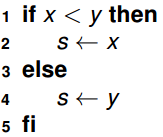
\includegraphics[scale=0.6]{images/if.png}\\
	\vspace{0.2cm}\p
	Eine \textbf{while}-Schleife\\
	\vspace{0.2cm}
	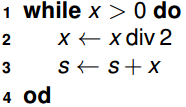
\includegraphics[scale=0.6]{images/while.png}\\
	\vspace{0.2cm}\p
	Eine \textbf{for}-Schleife\\
	\vspace{0.2cm}
	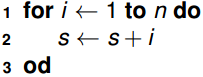
\includegraphics[scale=0.6]{images/for.png}
\end{frame}

\begin{frame}{Was kann man mit Algorithmen machen?}
	\begin{itemize}
		\pitem Komplexe Algorithmen mit Pseudocode definieren zu Sortierung, Graphen, Datenstrukturen\ip, im Modul \markBlue{Algorithmen I}
		\pitem Laufzeitanalyse von Algorithmen\ip, später.
		\pitem Korrektheitsbeweise\ip, jetzt.
	\end{itemize}
\end{frame}

\begin{frame}{Korrektheitsbeweise}
	\ip Wie findet man heraus, ob ein Algorithmus korrekt funktioniert?
	\begin{itemize}
		\pitem Durch den Beweis von Zusicherungen, die an bestimmten Stellen des Algorithmus gelten.
	\end{itemize}

	\vertspace

	\bp Was sind Zusicherungen?
	\begin{itemize}
		\pitem prädikatenlogische Formeln, die Aussagen über (Zusammenhänge zwischen) Variablen machen
	\end{itemize}
\end{frame}



%	\begin{frame}
%	\textbf{Beispiel}\\
%	Was ist hier die Schleifeninvariante?\\
%	\vspace{0.1cm}
%		Seien $a,b \in \mathbb{N}_0$\\
%		$x \leftarrow b$\\
%		$x \leftarrow a$\\
%		$while$ $y \neq 0$\\
%		do \\
%		\hspace{0.4cm} $y \leftarrow y - 1$\\
%		\hspace{0.4cm} $x \leftarrow x + 1$\\
%		od
%	\end{frame}


\subsection{Das Hoare-Kalkül}
\begin{frame}{Das Hoare-Tripel}
	\p
	
	\begin{block}{Definition}
		$\{P\}S\{Q\}$ heißt Hoare-Tripel. \ip Dabei gilt:
		\begin{itemize}
			\pitem S ist ein Programmstück im Pseudocode
			\pitem P und Q sind Zusicherungen
		\end{itemize}
	\end{block}
	\begin{itemize}
		\pitem P nennt man Vorbedingung, Q Nachbedingung
		\pitem Prädikatenlogische Formeln
		\pitem Beispiel (Vorausblick): $\{x \objequiv  1 \} x \leftarrow x + 1 \{x \objequiv 2\}$
		\pitem Meistens in jeder Zeile nur eine Zeile Code oder ein Zusicherungsblock
	\end{itemize}
\end{frame}

\begin{frame}{Das Hoare-Tripel}
	\begin{block}{Gültigkeit von Hoare-Tripeln}
		$\{P\}S\{Q\}$ ist gültig, wenn für jede gültige Interpretation $(D, I)$ und Variablenbelegung $\beta$ gilt:\\\bp
		Aus 
		\begin{itemize}
			\pitem $val_{D, I, \beta}(P) = w$
			\pitem $\beta'$ ist Variablenbelegung nach Ausführung von $S$
		\end{itemize}
		\ip folgt $val_{D, I, \beta'}(Q) = w$
	\end{block}
\end{frame}

\begin{frame}{Zuweisung}
	\begin{block}{Axiom HT-A}
		\begin{itemize}
			\pitem Sei $x \leftarrow E$ eine Zuweisung
			\pitem $Q$ eine Nachbedingung von $x \leftarrow E$ und
			\pitem $\sigma_{\{x/E\}}$ kollisionsfrei für Q
		\end{itemize}
		\p Dann ist $\sigma_{\{x/E\}}(Q) x \leftarrow E\{Q\}$ ein gültiges Hoare-Tripel
	\end{block}\p
	\textbf{Bemerkung}\\
	\begin{itemize}
		\pitem $\sigma_{\{x/E\}}$ ist die Substitution von $x$ mit $E$
		\pitem Bei Anwendung der Regel rückwärts vorgehen
	\end{itemize}
\end{frame}

\begin{frame}
	\textbf{Beispiel}\\
	Betrachte die Zuweisung \\
	$x \leftarrow x +1$\\
	und die Nachbedingung\\
	$\{x \dot = 1\}$\\
	\ip Nach HT-A gilt\\
	\pause
	$\{x+1 \dot = 1\}$ $ x \leftarrow x + 1$ $ \{x \dot = 1\}$ ist ein gültiges Hoare-Tripel.
\end{frame}

\begin{frame}{Ableitungsregeln: HT-E}
	\begin{itemize}
		\item Verstärkung der Vorbedingung
		\item Abschwächung der Nachbedingung
	\end{itemize}\p
	\begin{block}{HT-E}
		Wenn $\{P\}S\{Q\}$ ein gültiges Hoare-Tripel ist und $P' \vdash P$ und $Q \vdash Q'$ gelten, dann folgt:\\
		\pause
		$\{P'\}S \{Q'\}$ ist ein gültiges Hoare-Tripel.
	\end{block}
	\p\textbf{Bemerkung}\\
	$B \vdash A :\Leftrightarrow$ Aussage $A$ ist syntaktisch aus Aussage $B$ ableitbar
\end{frame}

\begin{frame}
	\textbf{Beispiel}\\
	Angenommen es sei $\{y > 3\}$ $x \leftarrow y-1$ $\{x > 1\}$ ein gültiges Hoare-Tripel.\\
	Es gilt $\{(y>4)\} \vdash \{(y>3)\} $ und $\{(x>1)\} \vdash \{(x>0)\} $.\\
	Also folgt nach HT-E:\\
	\pause
	$\{y > 4\}$ $x \leftarrow y-1$ $\{x > 0\}$ ist ein gültiges Hoare-Tripel.\\
	\pause
	\vertspace
	\textbf{Bemerkung}\\
	Es müssen sich nicht unbedingt beide Bedingungen ändern! \\
	Aus $\{(y>3)\} \vdash \{(y>3)\} $ und $\{(x>1)\} \vdash \{(x>0)\} $ \\folgt nach HT-E auch \\
	$\{y > 3\}$ $x \leftarrow y-1$ $\{x > 0\}$ ist ein gültiges Hoare-Tripel.
\end{frame}

\begin{frame}{Ableitungsregeln: HT-S}
	\p Hintereinanderausführung von durch Hoare-Triple bewiesene Code Segmente sind selbst gültig.\p
	\begin{block}{HT-S}
		Wenn $\{P\}S_1\{Q\}$ und $\{Q\}S_2\{R\}$ gültige Hoare-Tripel sind\ip, dann folgt:\ip $\{P\}S_1; S_2\{R\}$ ist ein gültiges Hoare-Tripel. 
	\end{block}
	\p\textbf{Bemerkung}\\
	";"  \space trennt hier zwei Programmstücke
\end{frame}

\begin{frame}
	\textbf{Beispiel}\\
	Angenommen es seien $\{y > 3\}$ $x \leftarrow y-1$ $\{x > 1\}$ und \\
	$\{x > 1\}$ $z \leftarrow x-1$ $\{z > -1\}$ gültige Hoare-Tripel.\\
	\ip Dann folgt nach HT-S:\\
	\pause
	$\{y > 3\}$ $x \leftarrow y-1; z \leftarrow x-1$ $\{z > -1\}$ ein gültiges Hoare-Tripel.
\end{frame}

\begin{frame} {Bedingte Anweisungen}\p
	\begin{block}{HT-I}
		Wenn $\{P \land B\}S_1\{Q\}$ und $\{P \land \lnot B\}S_2\{Q\}$ gültige Hoare-Tripel sind\ip, dann folgt:\\
		
		\vertspace
		\quad$\{P\}$\\
		\qquad\textbf{if} $B$ \textbf{then} $S_1$ \\
		\qquad\textbf{else} $S_2$\\
		\qquad\textbf{fi}\\
		\quad$\{Q\}$\\
		\vertspace
		
		
		ist ein gültiges Hoare-Tripel.
	\end{block}
\end{frame}

\begin{frame}{Beispiel}
	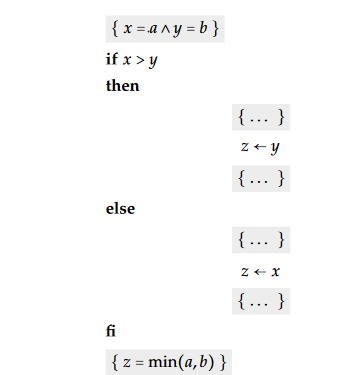
\includegraphics[scale=0.6]{images/if_fi.PNG}
\end{frame}		

\begin{frame}{Beispiel}
	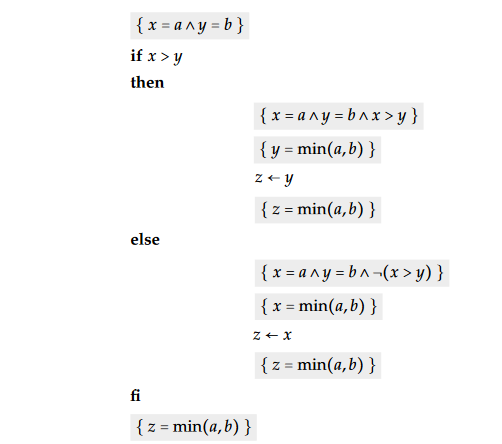
\includegraphics[scale=0.6]{images/if_fi_loes.PNG}
\end{frame}		

%\begin{frame}{Weiteres Beispiel}
%Sei $p$ eine Person, $betrunken(p)$ ein einstelliges Prädikat mit $betrunken(p) = wahr %:\Leftrightarrow getrunkeneGl"uhweins \objequiv 20$.
%\begin{algorithm}
%	$\{getrunkeneGl"uhweins = 0\}$
%	\While{$\lnot betrunken(p)$}{$getrunkeneGl"uhweins \leftarrow getrunkeneGl"uhweins + 1$}
%\end{algorithm}
%\end{frame}

\begin{frame} {Schleifen}
	\begin{block}{HT-W}
		Wenn $\{I \land B\}S\{I\}$ ein gültiges Hoare-Tripel ist\ip, dann folgt:\\\ip
		
		\vertspace
		$\{I\}$\\
		\textbf{while} $B$
		\textbf{do} $S$ \\
		\textbf{od}\\
		$\{I \land \lnot B\}$\\
		\vertspace
		
		ist ein gültiges Hoare-Tripel.
	\end{block}
\end{frame}

\begin{frame}{Schleifeninvariante}
	\begin{itemize}
		\pitem Eine spezielle Zusicherung
		\pitem Schleifeninvarianten müssen \textbf{vor}, \textbf{während} und \textbf{nach} jedem Schleifendurchlauf gelten
		\pitem Garantiert, dass die Schleife nicht während einem beliebigen Durchlauf ``kaputt'' geht.
		%\pitem Sie \textbf{müssen nicht} während des Schleifendurchlaufs gelten (können aber)
	\end{itemize}
\end{frame}

\begin{frame}
	\textbf{Beispiel}\\
	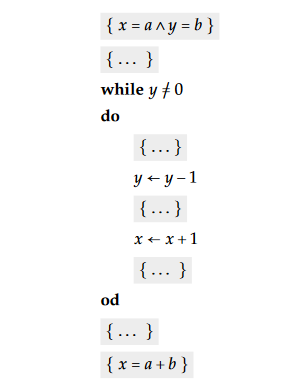
\includegraphics[scale=0.7]{images/do_od.PNG}
\end{frame}

\begin{frame}
	\textbf{Beispiel}\\
	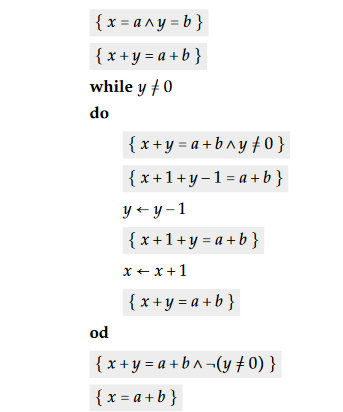
\includegraphics[scale=0.7]{images/do_od_loes.png}
\end{frame}

\begin{frame}
    Bestimmt für den folgenden Algorithmus was er berechnet und eine 
Schleifeninvariante: \\
$\{a \in \N_+, b \in \N_+\}$ \\
$X_0 \leftarrow a$ \\
$Y_0 \leftarrow b $\\
$P_0 \leftarrow 1 $\\
$\alpha_0 \leftarrow X_0 mod  2$ \\
$n \leftarrow 1 + \lceil log_2 a \rceil $\\
$for i \leftarrow 0$ to $n-1 do $ \\
\hspace{5mm}
$P_{i+1} \leftarrow P_i * {Y_i}^{\alpha_i}$ \\
\hspace{5mm}
$X_{i+1} \leftarrow X_i div 2$ \\
\hspace{5mm}
$Y_{i+1} \leftarrow {Y_i}^2$ \\
\hspace{5mm}
$\alpha_{i+1} \leftarrow X_{i+1} mod 2$ \\
od 
\newline \newline
Tipp: Beispieleingabe $a = 5$ und $b = 2$
\end{frame}



\begin{frame}
	
\includegraphics[width=\linewidth]{../images/thatsall.png}
\end{frame}


\end{document}
\def\tutdate{16.12.2011}

\documentclass[handout]{beamer}
\usepackage{../templates/beamerthemekitwide}
%\usepackage{enumitem}

\usepackage[utf8]{inputenc}
\usepackage[T1]{fontenc}
\usepackage[ngerman]{babel}
\usepackage{listings}
\usepackage{hyperref}
\usepackage{graphicx}

\usepackage{amsmath}
\usepackage{amsthm}
\usepackage{amssymb}
\usepackage{polynom}

%\usepackage{ifthen}
%\usepackage{adjustbox} % for \adjincludegraphics

%\usepackage{tikz}
\usepackage{listings}

%\usepackage[]{algorithm2e}

%\usepackage{colortbl}
\usepackage{verbatim}
%\usepackage{alltt}
%\usepackage{changes}

%\usepackage{pdfpages}
%\usepackage{tabularx}

%\usepackage{euler}


\newcommand{\markBlue}[1]{\textcolor{kit-blue100}{#1}}
\newcommand{\markGreen}[1]{\textcolor{kit-green100}{#1}}
\newcommand{\vertspace}{\vspace{.2cm}}

%\newcommand{\#}{\markBlue{#1}}

%\newcommand{\pitem}{\pause\item}
\newcommand{\p}{\pause}

% -- MATH MACROS
\newcommand{\thistheoremname}{}
\newcommand{\G}{\mathbb{Z}}
\newcommand{\B}{\mathbb{B}}
\newcommand{\R}{\mathbb{R}}
\newcommand{\N}{\mathbb{N}}
\newcommand{\Q}{\mathbb{Q}}
\newcommand{\C}{\mathbb{C}}
\newcommand{\Z}{\mathbb{Z}}
\newcommand{\F}{\mathbb{F}}
\newcommand{\mi}{\mathrm{i}}
\renewcommand{\epsilon}{\varepsilon}
\newcommand{\okalk}{\mathscr{O}}


\newenvironment<>{taskblock}[1]{%
	\setbeamercolor{block title}{fg=kit-orange15,bg=kit-orange100}
	\setbeamercolor{block body}{fg=black,bg=kit-orange30}%
	\begin{block}#2{#1}}{\end{block}}

\setbeamertemplate{enumerate items}[default]

% Aussagenlogik Symbole
\newcommand{\W}{w}
\renewcommand{\F}{f}

% Kodierung
\newcommand{\frepr}{\textbf{repr}}
\newcommand{\fRepr}{\textbf{Repr}}
\newcommand{\fZkpl}{\textbf{Zkpl}}
\newcommand{\fbin}{\textbf{bin}}
\newcommand{\fdiv}{\textbf{ div }}
\newcommand{\fmod}{\textbf{ mod }}

% Speicherabbild
\newenvironment{memory}{\begin{tabular}{r | l}Adresse&Wert\\\hline\hline}{\end{tabular}}
\newcommand{\memrow}[2]{#1 & #2 \\\hline}

% Praedikatenlogik
\newcommand{\objequiv}{\stackrel{\cdot}{=}}
\newcommand{\pval}{val_{D,I,\beta}}

% Neue Befehle
\newcommand{\ip}{\pause} % inline pause, für mitten im satz
\newcommand{\pitem}{\pause\item} % für aufzählungen
\newcommand{\bp}{\pause} % block pause, für zwischen blöcken
\title[Grundbegriffe der Informatik]{ICPC\\Gruppe 2}
\date{\tutdate}
\subtitle{\tutTitle}
\author{Elias Schaut, Dennis Kobert, Niklas Kniep, Lam Vo, Ilia Bozhinov}

\institute{}

\titleimage{bg}
%\titleimage{bg-advent}

%
\ifthenelse{\equal{\compiletype}{livebeamer}}
	{
		\def\livebeamermode{1}
	}{}

\ifthenelse{\equal{\compiletype}{print}}
	{
		\def\printmode{1}
	}{}

\setbeamercovered{invisible}

%\usepackage[citestyle=authoryear,bibstyle=numeric,hyperref,backend=biber]{biblatex}
%\addbibresource{templates/example.bib}
%\bibhang1em

	
\def\tutTitle{Graphen I}
\begin{document}

\selectlanguage{ngerman}

%title page
\begin{frame}
	\titlepage
\end{frame}

\section{Graphen}
\begin{frame}{Graphen}
	\begin{block}{Definition: Graph}
		\ip Ein Graph $G = (V,E)$ ist ein Tupel aus:
		\begin{itemize}
			\pitem Einer endlichen, nichtleeren Knotenmenge $V$
			\pitem Einer endlichen Kantenmenge $E \subseteq V \times V$
		\end{itemize}
	\end{block}
	
	\bp
	
	Beispiel: Knotenmenge $V := \{a, b, c, d\}$. Kantenmenge könnte zum Beispiel sein...
	
	\begin{itemize}
		\pitem $E := \{(a,b), (c, d), (a, d)\}$
		\pitem $E := \{(a,a), (b,b), (c,c)\}$
		\pitem $E := \emptyset$
	\end{itemize}
\end{frame}

\begin{frame}{Wie sehen diese Graphen aus?}
	Beispiel: Knotenmenge $V := \{a, b, c, d\}$. Kantenmenge könnte zum Beispiel sein...
	\begin{itemize}
		\pitem $V := \{a, b, c, d\}, E := \{(a,b), (c, d), (a, d)\}$\\
		\p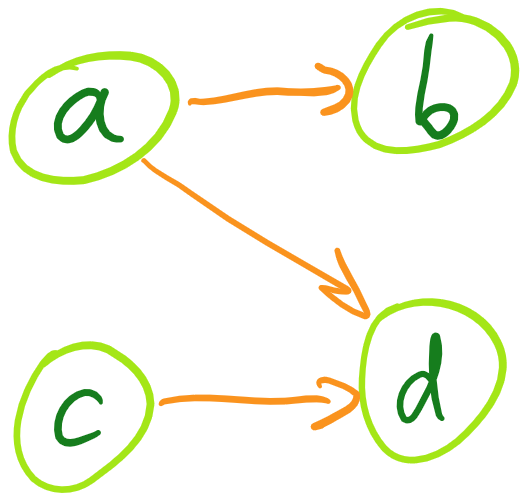
\includegraphics[scale=0.17]{images/graph_0_01.png}
		\pitem $V := \{a, b, c, d\}, E := \{(a,a), (b,b), (c,c)\}$\\
		\p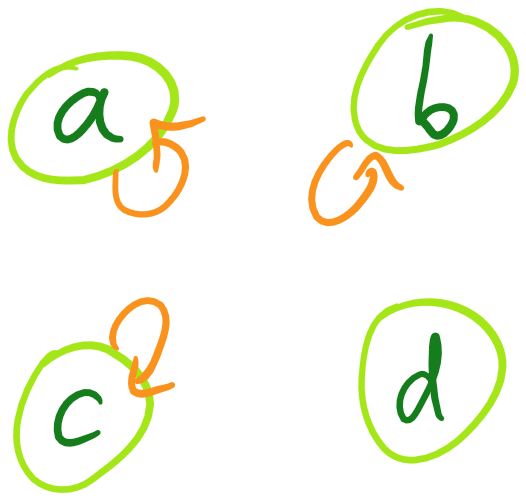
\includegraphics[scale=0.17]{images/graph_0_02.png}
		\pitem $V := \{a, b, c, d\}, E := \emptyset$\\
		\p
\includegraphics[scale=0.17]{images/graph_0_03.png}
	\end{itemize}
\end{frame}

\begin{frame}{Wann Angabe als Menge, wann als Visualisierung?}
	Wir verwenden gezeichnete Graphen und deren Definition als Mengen als äquivalent.
	
	\begin{itemize}
		\pitem $\{(a,b),(c,d),(a,d)\} = \{(a,b),(a,d),(c,d)\} \neq \{(b,a),(d,c),(d,a)\}$, also Kantenmenge mit unterschiedlichen Reihenfolgen darstellbar. Genauso die Knotenmenge.
	\end{itemize}

	\ip
	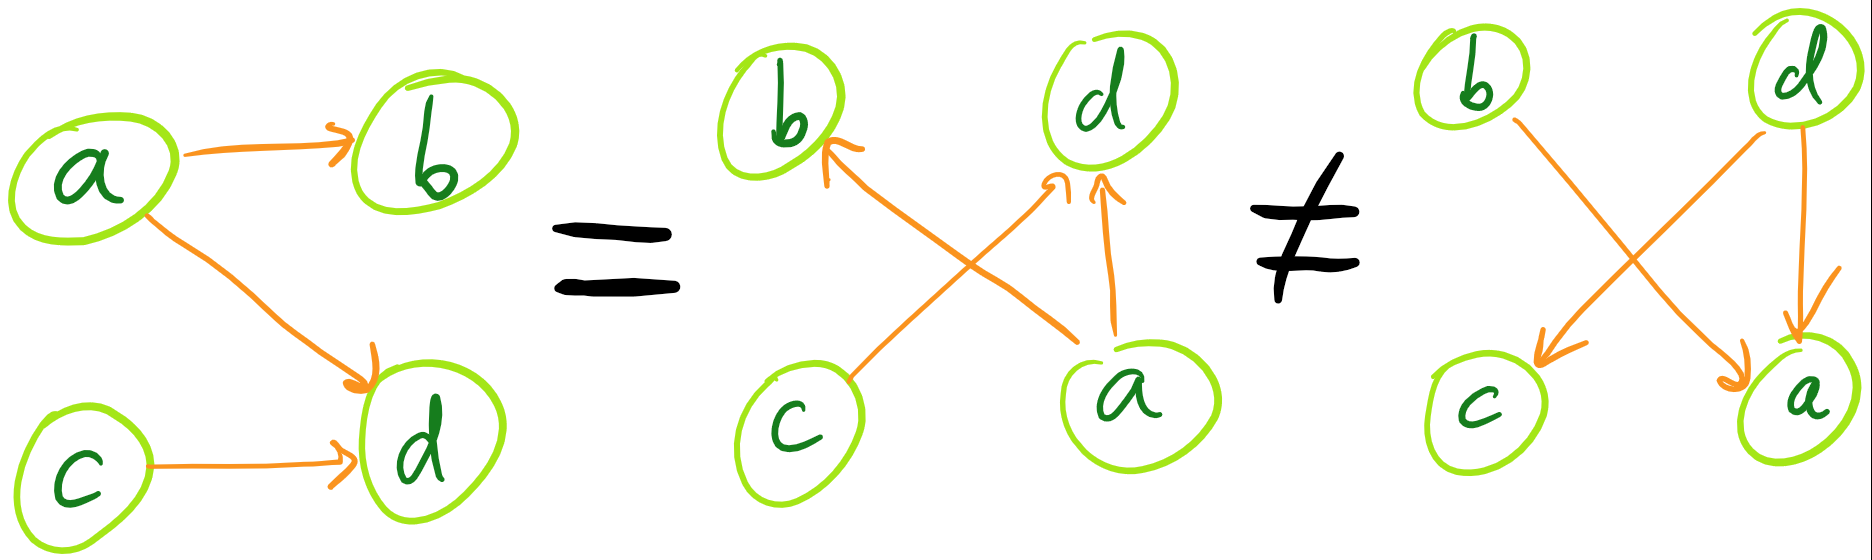
\includegraphics[scale=.3]{images/graph_1.png}
	
	\bp
	
	Es kann also in jedem Fall der Graph sowohl als ``Visualisierung'' oder als Menge angegeben werden, beide Varianten sind formal korrekt.
\end{frame}

\subsection{Praxisbeispiele}
% Hier bei allen Aussagen fragen, was die Tutanden als Ideen haben, wie man das als Graphenfrage formulieren kann
% Einige Sachen werden vorgegriffen (Wurzel, Knotengrad). Trotzdem fragen, Tutanden werden es vermutlich einfach komplizierter formulieren. Das so stehen lassen und erwähnen, dass darauf später genauer eingegangen wird.
% Dabei soll deutlich werden, dass konkrete Probleme in "die Sprache der Graphen" überführt werden kann und als bekanntes Problem gelöst werden kann

\begin{frame}{Praxisbeispiel: Soziales Netzwerk}
	\ip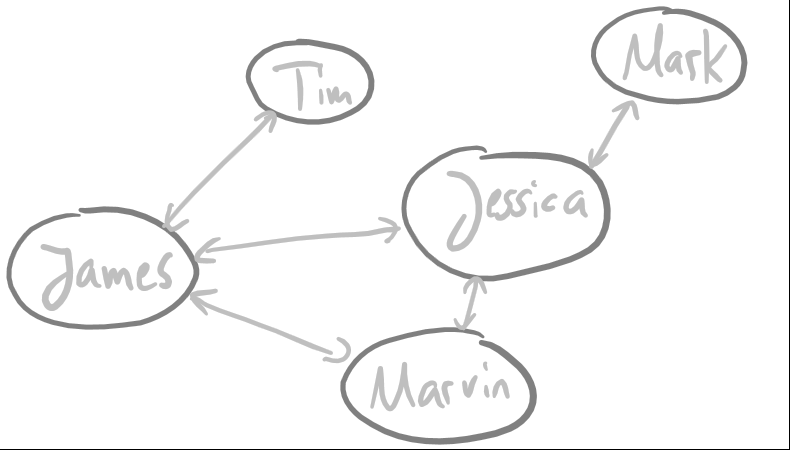
\includegraphics[scale=0.4]{images/graph_beispiel_socialnetwork.png}
	\begin{itemize}
		\pitem Ist Person $A$ direkt mit Person $B$ befreundet? \pause $\Leftrightarrow$ Gibt es eine Kante $(A,B)$?
		\pitem Ist Person $A$ über maximal 2 verschiedene Leute mit Person $B$ befreundet?\pause $\Leftrightarrow$  Gibt es einen Pfad von $A$ nach $B$ mit maximaler Länge 3?
		\pitem Wieviele Freunde hat Person $A$?\pause $\Leftrightarrow$ Welchen Grad hat Person $A \in V$?
	\end{itemize}
\end{frame}

\begin{frame}{Praxisbeispiel: Wie kommt man am schnellsten von $A$ nach $B$}
	\ip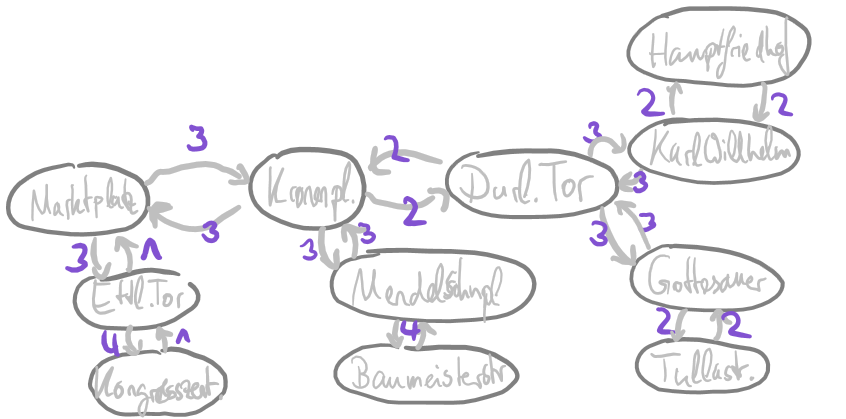
\includegraphics[scale=0.4]{images/graph_beispiel_kvv.png}
	\begin{itemize}
		\pitem Kantengewichtung: Jeder Kante wird eine Zahl $c \in \R$ zugewiesen.
		\pitem Wie lange dauert der kürzeste Weg von Kongresszentrum nach Hauptfriedhof? \pause $\Leftrightarrow$ Wie lang ist ein kürzester Pfad von Kongresszentrum nach Hauptfriedhof?
		\pitem Wo kommt man von Kronenplatz überall innerhalb von 5 Zeiteinheiten hin? \pause $\Leftrightarrow$ Für welche Orte $v \in V$ existiert ein Pfad $(Kronenplatz, ..., v)$ mit einer Länge von maximal 5?
	\end{itemize}
\end{frame}

\begin{frame}{Praxisbeispiel: Huffman-Bäume}
	\ip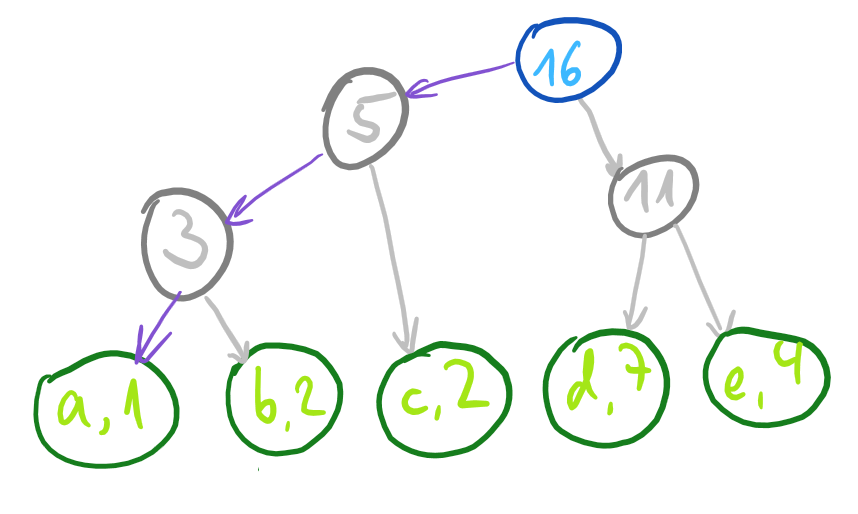
\includegraphics[scale=0.4]{images/graph_beispiel_huffman.png}
	\begin{itemize}
		\pitem Wie lang ist die Kodierung vom Zeichen $c$?\pause $\Leftrightarrow$ Wie lang ist der Pfad von Wurzel zu Knoten $c$? In diesem Fall $2$.
		\pitem Wie viele Zeichen werden kodiert? \pause $\Leftrightarrow$ Wie viele Knoten sind von der Wurzel erreichbar, die selbst keine ausgehenden Kanten haben? \pause $\Leftrightarrow$ Wie viele Blätter hat der Baum?
	\end{itemize}
\end{frame}


\subsection{Ungerichtete Graphen}
\begin{frame}{Ungerichtete Graphen}
	\begin{itemize}
		\pitem Bis jetzt\ip: Gerichtete Graphen, dh. Kanten $(u,v)$ hatten eine Richtung von Knoten $u$ nach Knoten $v$.
	\end{itemize}

	\bp
	
	\begin{block}{Ungerichteter Graph}
		Ein ungerichteter Graph ist ein Graph, dessen Kanten Mengen, und keine Tupel sind.
	\end{block}

	\bp
	
	\begin{itemize}
		\item Beispiel: Statt Kante $(u,v)$ jetzt Kante $\{u,v\} \pause = \{v, u\}$.
		\pitem Information über Richtung geht also verloren, Kanten verbinden nur noch Knoten, ohne sich zu merken, welcher Knoten Start und welcher Ziel ist.
	\end{itemize}
\end{frame}

\subsection{Begriffe}

\begin{frame}{Teilgraph}
	\begin{block}{Teilgraph}
		\ip Zu einem Graph $G := (V, E)$ ist ein Teilgraph definiert als $G' = (V', E')$, falls gilt $V' \subseteq V$ und $E' \subseteq V' \times V' \cap E$.
	\end{block}

	\bp	

	\begin{itemize}
		\item Beispiel: Sei $G := (V,E)$ mit $V := \{a,b,c,d,e,f\}$ und $E := \{(b,a),(b,f),(f,d),(e,f),(f,a),(e,b),(a,e),(f,c),(a,c),(c,a),(c,e)\}$
		\p\item Ist ein Graph mit $V_1:=\{a,c,d,e,f\}, E_1:= \{(a,c),(c,a),(a,e),(f,d)\}$ ein Teilgraph von $G$?
		\p\item Ist ein Graph mit $V_2:=\{d,f\}, E_2:= \{(f,d)\}$ ein Teilgraph von $G$?
		\p\item Ist ein Graph mit $V_3=E_3=\emptyset$ ein Teilgraph von $G$?
	\end{itemize}

	\bp
	
	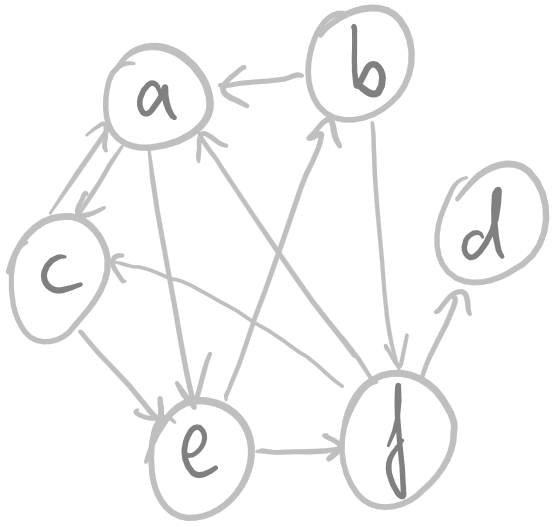
\includegraphics[scale=0.2]{images/graph_teilgraph_01.png}\ip
	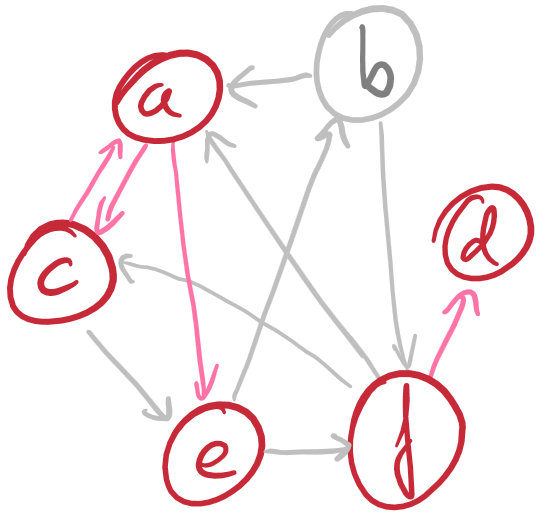
\includegraphics[scale=0.2]{images/graph_teilgraph_02.png}\ip
	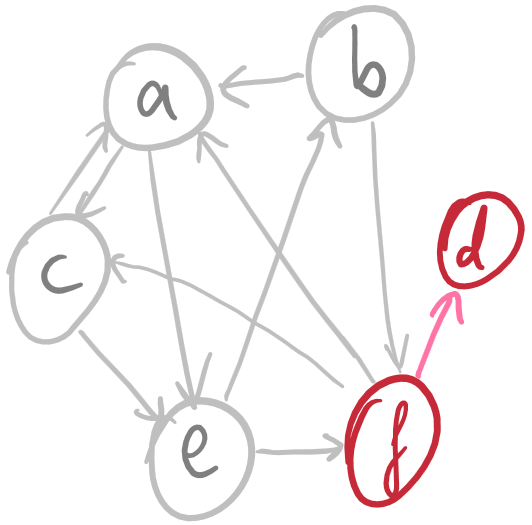
\includegraphics[scale=0.2]{images/graph_teilgraph_03.png}\ip
	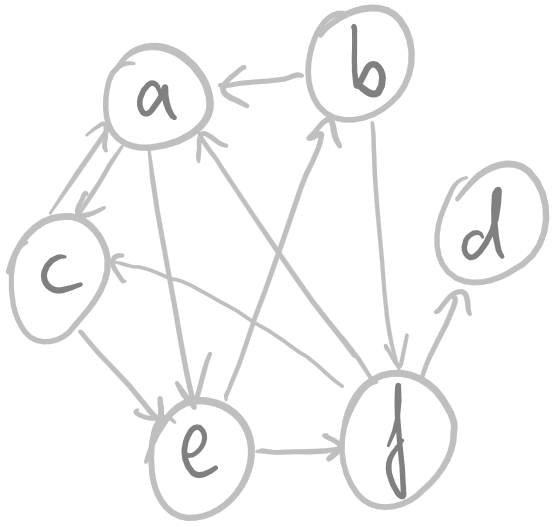
\includegraphics[scale=0.2]{images/graph_teilgraph_01.png} % Das ist technisch noch der letzte graph mit leeren kanten/knoten mengen
\end{frame}

\begin{frame}{Teilgraph}
	\begin{block}{Teilgraph}
		Zu einem Graph $G := (V, E)$ ist ein Teilgraph definiert als $G' = (V', E')$, falls gilt $V' \subseteq V$ und $E' \subseteq V' \times V' \cap E$.
	\end{block}
	
	\begin{itemize}
		\item Beispiel: Sei $G := (V,E)$ mit $V := \{a,b,c,d,e,f\}$ und $E := \{(b,a),(b,f),(f,d),(e,f),(f,a),(e,b),(a,e),(f,c),(a,c),(c,a),(c,e)\}$
		\p\item Ist ein Graph mit $V_4:=\{a,b\}, E_4:= \{(f,d)\}$ ein Teilgraph von $G$?
		\p\item Ist ein Graph mit $V_5:=\{g,a\}, E_5:=\{(g,a),(a,g)\}$ ein Teilgraph von $G$?
		% Beides nicht.
	\end{itemize}
\end{frame}

\begin{frame}{Pfad/Weg}
	\begin{columns}
		\begin{column}{0.6\textwidth}
			\begin{block}{Pfad informell}
				Ein Pfad(gerichtet)/Weg(ungerichtet) $(u,...,v)$ ist eine Aneinanderreihung von Knoten, die jeweils mit Kanten verbunden sind, sodass man über das \markGreen{traversieren} der Kanten vom Startknoten $u\in V$ zum Zielknoten $v\in V$ kommt.
			\end{block}
			
			\bp
			Anmerkung: Wenn man sich einen Knoten $x \in V$ merkt und eine Kante $(x,y) \in E$ traversiert, so gelangt man zu Knoten $y$.
			\bp
			
			\begin{block}{Pfad/Weg formell}
				Ein Pfad/Weg $P := (v_0, v_1, ..., v_n)$ der Länge $n$ ist eine Permutation auf $V$ , wobei gilt: $\forall i \in \Z_n: (v_i, v_{i+1}) \in E$.
			\end{block}	
		\end{column}
		
		\begin{column}{0.4\textwidth}
			\bp
			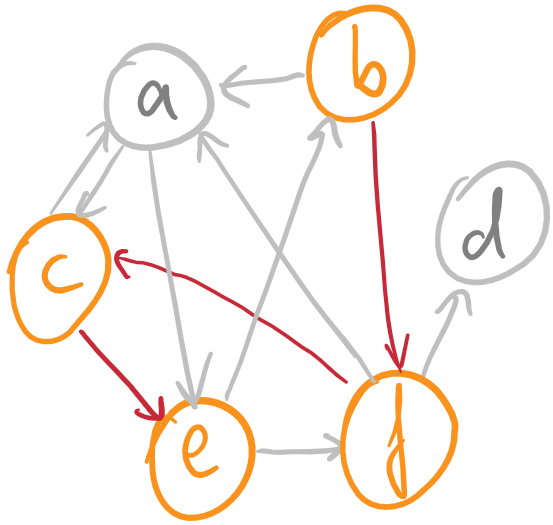
\includegraphics[scale=0.3]{images/graph_pfad.png}
			
			\ip Der Pfad $(b,f,c,e)$ ist ein möglicher Pfad von $b$ nach $e$ der Länge 3.
			
			\ip Gibt es noch andere solcher Pfade?
		\end{column}
	\end{columns}
\end{frame}


\begin{frame}{Zyklus/Kreis}
	\begin{block}{Zyklus/Kreis}
		\ip Ein Zyklus(gerichtet)/Kreis(ungerichtet) ist ein Pfad/Weg $(v_1, ..., v_n)$ mit $v_1 = v_n$.
	\end{block}
	\bp
	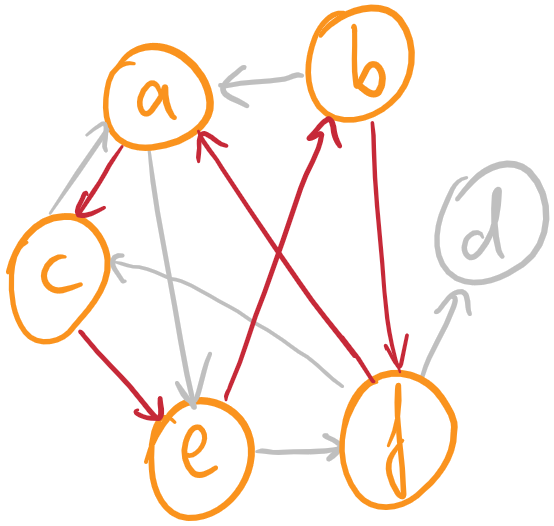
\includegraphics[scale=0.3]{images/graph_zyklus.png}
	
	\ip Der Pfad $(b,f,a,c,e)$ ist ein möglicher Zyklus.
	
	\ip Gibt es noch andere Zyklen?
\end{frame}

\begin{frame}{Zusammenhängend}

	% Jeweils Beispiele an der Tafel vormalen.

	\bp
	
	\begin{block}{Zusammenhängender Graph}
		Ein ungerichteter Graph heißt zusammenhängend, wenn gilt: $\forall u,v \in V \exists$ Pfad von $u$ nach $v$.
	\end{block}

	\bp

	\begin{block}{Stark zusammenhängender Graph}
		Ein gerichteter Graph heißt stark zusammenhängend, wenn gilt: $\forall u,v \in V \exists$ Pfad von $u$ nach $v$.
	\end{block}

	\bp
	
	\begin{block}{Schwach zusammenhängender Graph}
	Ein gerichteter Graph heißt schwach zusammenhängend, wenn der zugehörige ungerichteter Graph zusammenhängend ist.
	\end{block}
\end{frame}

\begin{frame}{Knotengrad}
	
	% Jeweils Beispiele an der Tafel vormalen.
	
	\begin{block}{Eingangsgrad}
		Der Eingangsgrad eines Knoten $u \in V$ ist definiert als: $d_{-}(u) := |\{(v, u) \in E: v \in V\}|$\ip, also die Anzahl der Kanten, die in den Knoten $u$ zeigen.
	\end{block}

	\bp 

	\begin{block}{Ausgangsgrad}
	Der Ausgangsgrad eines Knoten $u \in V$ ist definiert als: $d_{+}(u) := |\{(u, v) \in E: v \in V\}|$\ip, also die Anzahl der Kanten, die vom Knoten $u$ aus weg zeigen.
	\end{block}

	\bp
	
	\begin{block}{Grad}
		Der Grad eines Knoten $u$ ist definiert als: $d(u) := d_{+}(u) + d_{-}(u)$\ip, also die Anzahl der Kanten, über die $u$ verbunden ist.
	\end{block}
\end{frame}

\begin{frame}{Bäume}
	
	% Jeweils Beispiele an der Tafel vormalen.
	
	\begin{itemize}
		\pitem Kennt ihr schon: Huffman-Baum
	\end{itemize}

	\begin{block}{Gerichteter Baum}
	Ein gerichteter Baum ist ein gerichteter Graph, der einen Knoten v besitzt, sodass zu jedem Knoten u ein eindeutiger Pfad von v nach u existiert
	\end{block}

	\bp

	\begin{block}{Ungerichteter Baum}
		Ein ungerichteter Baum ist ein \markGreen{zusammenhängender kreisfreier} ungerichteter Graph.	
	\end{block}

	\bp

	\begin{itemize}
		\pitem Bäume haben immer einen Wurzelknoten, von dem alle anderen Knoten ausgehen.
		\pitem Ungerichtete Bäume \markBlue{können} mehrere Wurzeln haben.
		\pitem Knoten mit Grad 1 heißen Blätter.
	\end{itemize} 
\end{frame}



\begin{frame}{Randfälle}
	\begin{itemize}
		\pitem Wieviele Kanten kann ein Graph mit $n$ Knoten maximal haben? \pause $n^2$
		\pitem Wieviele Kanten kann ein schlingenfreier Graph mit $n$ Knoten maximal haben? \pause $n^2-n \p = n(n-1)$
		\pitem Wieviele Kanten kann ein ungerichteter Graph mit $n$ Knoten maximal haben? \pause $\frac{n(n-1)}{2} + n\p = \frac{n(n+1)}{2}$
		\pitem Wieviele Kanten kann ein ungerichteter schlingenfreier Graph mit $n$ Knoten maximal haben? \pause $\frac{n(n-1)}{2}$
	\end{itemize}
\end{frame}

\begin{frame}{Isomorphismen}
\begin{block}{Isomorphismus}
	Zwei Graphen sind isomorph zueinander, wenn ein Isomorphismus (Bijektion) f zwischen ihren Knoten existiert, sodass: $(x, y) \in E_1 \leftrightarrow (f(x), f(y)) \in E_2$
	\newline
	Informal: Man benennt die Knoten des einen Graphen so um, dass der andere Graph dabei herauskommt.
\end{block}
\end{frame}

\begin{frame}
	
\includegraphics[width=\linewidth]{../images/thatsall.png}
\end{frame}


\end{document}

\def\tutdate{13.01.2019}

\documentclass[]{beamer}
\usepackage{../templates/beamerthemekitwide}
%\usepackage{enumitem}

\usepackage[utf8]{inputenc}
\usepackage[T1]{fontenc}
\usepackage[ngerman]{babel}
\usepackage{listings}
\usepackage{hyperref}
\usepackage{graphicx}

\usepackage{amsmath}
\usepackage{amsthm}
\usepackage{amssymb}
\usepackage{polynom}

%\usepackage{ifthen}
%\usepackage{adjustbox} % for \adjincludegraphics

%\usepackage{tikz}
\usepackage{listings}

%\usepackage[]{algorithm2e}

%\usepackage{colortbl}
\usepackage{verbatim}
%\usepackage{alltt}
%\usepackage{changes}

%\usepackage{pdfpages}
%\usepackage{tabularx}

%\usepackage{euler}


\newcommand{\markBlue}[1]{\textcolor{kit-blue100}{#1}}
\newcommand{\markGreen}[1]{\textcolor{kit-green100}{#1}}
\newcommand{\vertspace}{\vspace{.2cm}}

%\newcommand{\#}{\markBlue{#1}}

%\newcommand{\pitem}{\pause\item}
\newcommand{\p}{\pause}

% -- MATH MACROS
\newcommand{\thistheoremname}{}
\newcommand{\G}{\mathbb{Z}}
\newcommand{\B}{\mathbb{B}}
\newcommand{\R}{\mathbb{R}}
\newcommand{\N}{\mathbb{N}}
\newcommand{\Q}{\mathbb{Q}}
\newcommand{\C}{\mathbb{C}}
\newcommand{\Z}{\mathbb{Z}}
\newcommand{\F}{\mathbb{F}}
\newcommand{\mi}{\mathrm{i}}
\renewcommand{\epsilon}{\varepsilon}
\newcommand{\okalk}{\mathscr{O}}


\newenvironment<>{taskblock}[1]{%
	\setbeamercolor{block title}{fg=kit-orange15,bg=kit-orange100}
	\setbeamercolor{block body}{fg=black,bg=kit-orange30}%
	\begin{block}#2{#1}}{\end{block}}

\setbeamertemplate{enumerate items}[default]

% Aussagenlogik Symbole
\newcommand{\W}{w}
\renewcommand{\F}{f}

% Kodierung
\newcommand{\frepr}{\textbf{repr}}
\newcommand{\fRepr}{\textbf{Repr}}
\newcommand{\fZkpl}{\textbf{Zkpl}}
\newcommand{\fbin}{\textbf{bin}}
\newcommand{\fdiv}{\textbf{ div }}
\newcommand{\fmod}{\textbf{ mod }}

% Speicherabbild
\newenvironment{memory}{\begin{tabular}{r | l}Adresse&Wert\\\hline\hline}{\end{tabular}}
\newcommand{\memrow}[2]{#1 & #2 \\\hline}

% Praedikatenlogik
\newcommand{\objequiv}{\stackrel{\cdot}{=}}
\newcommand{\pval}{val_{D,I,\beta}}

% Neue Befehle
\newcommand{\ip}{\pause} % inline pause, für mitten im satz
\newcommand{\pitem}{\pause\item} % für aufzählungen
\newcommand{\bp}{\pause} % block pause, für zwischen blöcken
\title[Grundbegriffe der Informatik]{ICPC\\Gruppe 2}
\date{\tutdate}
\subtitle{\tutTitle}
\author{Elias Schaut, Dennis Kobert, Niklas Kniep, Lam Vo, Ilia Bozhinov}

\institute{}

\titleimage{bg}
%\titleimage{bg-advent}

%
\ifthenelse{\equal{\compiletype}{livebeamer}}
	{
		\def\livebeamermode{1}
	}{}

\ifthenelse{\equal{\compiletype}{print}}
	{
		\def\printmode{1}
	}{}

\setbeamercovered{invisible}

%\usepackage[citestyle=authoryear,bibstyle=numeric,hyperref,backend=biber]{biblatex}
%\addbibresource{templates/example.bib}
%\bibhang1em

	
\def\tutTitle{O-Notation}
\begin{document}

\selectlanguage{ngerman}

\newcommand{\okalk}{\mathcal{O}}

%title page
\begin{frame}
	\titlepage
\end{frame}

\section{Komplexitätstheorie}

\begin{frame}{Komplexitätstheorie}
	\pause
	Wichtige Komplexitätsmaße:
	\begin{itemize}
		\pitem Speicherplatzbedarf
		\pitem Rechen- bzw. Laufzeit
	\end{itemize}
	Unterscheidung in
	\begin{itemize}
		\pitem Best Case (oft uninteressant)
		\pitem Average Case (schwierig zu finden, deswegen selten angegeben)
		\pitem Worst Case  (meistens angegeben)
	\end{itemize}
\end{frame} 

\subsection{O-Notation}
\begin{frame}{Ignorieren konstanter Faktoren}
	\begin{block}{Definition}
		Seien $g,f: \mathbb{N}_0 \rightarrow \mathbb{R}_0^+$ Funktionen. Dann wächst $g$ asymptotisch genauso schnell wie $f$ genau dann, wenn gilt:\\
		$\exists c, c' \in \mathbb{R}_+ : \exists n_0 \in \mathbb{N}_0: \forall n \geq n_0 : c \cdot f(n) \leq g(n)\leq c' \cdot f(n)$
	\end{block}
	\pause

	\textbf{Notation}\\
	$f \asymp g$ oder $f(n) \asymp g(n)$ ("asymptotisch gleich")\\
	\textbf{Bemerkung}\\
	$\asymp$ ist eine Äquivalenzrelation
\end{frame}

\begin{frame}{Theta}
	\begin{block}{Definition}
		$\Theta (f) = \{g|g \asymp f\}$
	\end{block}

	\pause
	
	\begin{block}{Satz}
		$\forall a, b \in \mathbb{R}_+ : \Theta (a\cdot f) = \Theta (b \cdot f)$
	\end{block}
\end{frame}

\begin{frame}{Obere und untere Schranke}
	\begin{block}{Obere Schranke (Worst-Case Approximation)}
		$O(f) = \{g| \exists c \in \mathbb{R}_+ : \exists n_0 \in \mathbb{N}_0: \forall n \geq n_0 : g(n)\leq c \cdot f(n)\}$
	\end{block}

	\pause
	
	\begin{block}{Untere Schranke (Best-Case Approximation)}
		$\Omega(f) = \{g| \exists c \in \mathbb{R}_+ : \exists n_0 \in \mathbb{N}_0: \forall n \geq n_0 : g(n)\geq c \cdot f(n)\}$
	\end{block}
	\pause
	\textbf{Notation}\\
	\begin{itemize}
		\item $g\curlyeqprec f$ falls $g \in O(f)$ bzw. g wächst asymptotisch höchstens so schnell wie f
		\item $g \curlyeqsucc f $ falls $g \in \Omega (f)$ bzw. g wächst asymptotisch mindestens so schnell wie f
	\end{itemize}
	\pause
	\textbf{Bemerkung}\\
	Es gilt $\Theta (f) = O(f) \cap \Omega (f)$
\end{frame}

\begin{frame}
	\begin{block}{Lemma}
		$log_a n \in \Theta (log_b n)$
	\end{block}
	\textbf{Beispiel}\\
	$log_2 n \in \Theta(log_8 n)$\\
	\pause
	\textbf{Beweis}\\
	$\frac{1}{3} log_2 n \ip= \frac{1}{log_2 8} log_2 n \ip= \frac{log_2 n}{log_2 8} \ip= log_8 n \leq log_2 n$
\end{frame}

\begin{frame}
	\textbf{Aufgabe}\\
	Gilt $log_2(n^{20}) \in \Theta (log \space n)$\\
	\pause
	\textbf{Lösung}\\
	Ja, denn $log_2 (n^{20}) = 20 \cdot log_2 n$
\end{frame}

\begin{frame}{Algorithmus von Warshall}
	\begin{columns}
		\begin{column}{0.7\textwidth}
			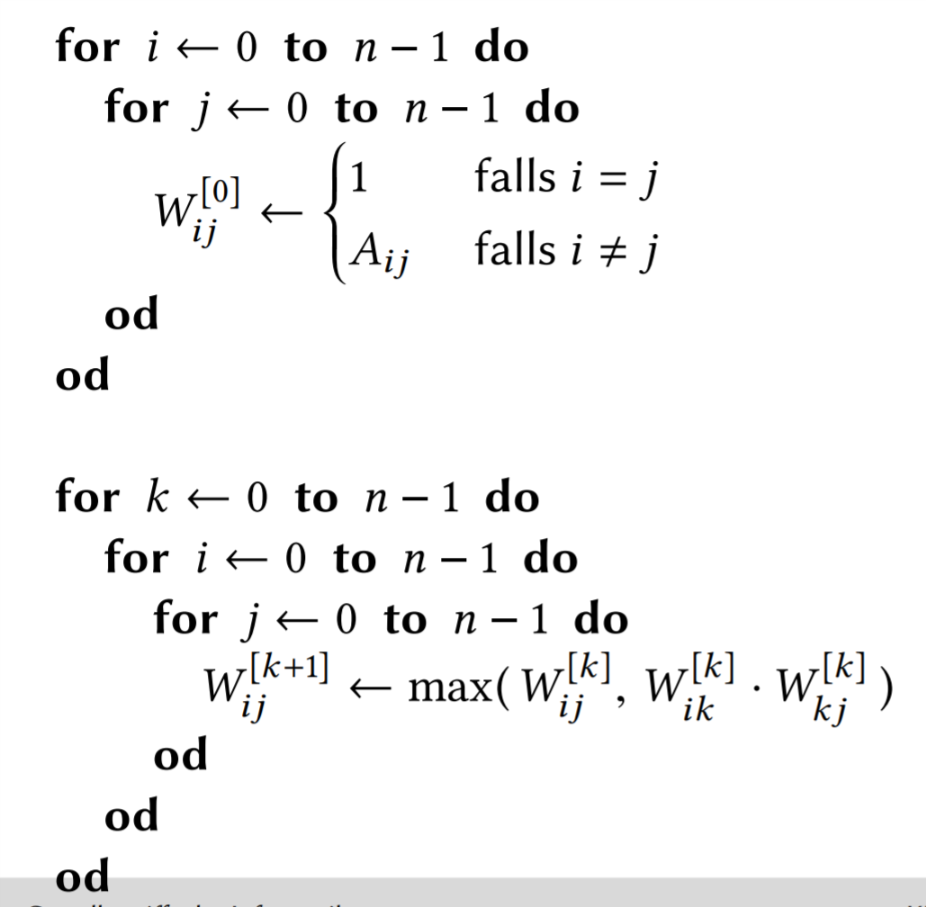
\includegraphics[scale=0.5]{images/warshall.png}\\
		\end{column}
		\begin{column}{0.3\textwidth}
			Wie schnell ist das ganze?
		\end{column}
	\end{columns}
\end{frame}

\begin{frame}
Gelten folgende Approximationen?

\begin{itemize}
	\pitem $4n^2 + \pi n + 2 \sqrt{n} \in \Theta(n^2)?$ \pause Ja.
	\pitem $4n^{2,1} + \pi n + 2 \sqrt{n} \in \Theta(n^2)?$ \pause Nein.
\end{itemize}

\bp Es sind immer nur die höchsten Faktoren interessant!

\begin{itemize}
	\pitem $4n^4 + 3c^6 \in \Theta(n^4)$? \pause Ja\ip, $c$ ist eine Konstante, $3c^6=(3c^6)n^0$ hat eine kleinere Potenz als $n^4$.
	\pitem $\log_{4213}(n) \in \Theta(\log_2(n))$ \pause Ja\ip, die Basis des Logarithmus ist im O-Kalkül egal.
	
	\begin{itemize}
		\pitem Grund: $\okalk(\log_b n) \ip= \okalk(\frac{\log_a n}{\log_a b}) \ip = \okalk(\frac{1}{\log_a b}\log_a n) \ip = \okalk(\log_a n)$.
	\end{itemize}
	
	\pitem $n! \in \Theta(n^{\pi e 2000})$ \pause Nein\ip, Fakultät wächst asymptotisch schneller als fast alles andere.
\end{itemize}
\end{frame}

\begin{frame}{Aufgabe}
\begin{taskblock}{Übungsaufgabe}
Entscheide für jede Zelle, ob die Formel der Zeile in der Menge der Spalte liegt.

\begin{center}
\begin{tabular}{r||c|c|c|c|c|c}%*{2}{>{$}c<{$}}|*{4}{>{$}c<{$}}
	\hline
	& $\okalk(n^3)$ & $\okalk(n)$ & $\Theta(c!)$ & $\Theta(n^\pi)$ & $\Omega(n^6)$ & $\Omega(n!)$ \\\hline\hline
	
	$2n^2 + 4n$ 
	& \visible<2->{$\in$}
	& \visible<3->{$\not\in$}
	& \visible<4->{$\not\in$}
	& \visible<5->{$\not\in$}
	& \visible<6->{$\not\in$}
	& \visible<7->{$\not\in$}
	\\\hline
	
	
	$\pi$
	& \visible<8->{$\in$}
	& \visible<9->{$\in$}
	& \visible<10->{$\in$}
	& \visible<11->{$\not\in$}
	& \visible<12->{$\not\in$}
	& \visible<13->{$\not\in$}
	\\\hline
	
	$\log(n)$
	& \visible<14->{$\in$}
	& \visible<15->{$\in$}
	& \visible<16->{$\not\in$}
	& \visible<17->{$\not\in$}
	& \visible<18->{$\not\in$}
	& \visible<19->{$\not\in$}
	\\\hline
	
	$n\log(n)$
	& \visible<20->{$\in$}
	& \visible<21->{$\not\in$}
	& \visible<22->{$\not\in$}
	& \visible<23->{$\not\in$}
	& \visible<24->{$\not\in$}
	& \visible<25->{$\not\in$}
	\\\hline
	
	$n^\pi$
	& \visible<26->{$\not\in$}
	& \visible<27->{$\not\in$}
	& \visible<28->{$\not\in$}
	& \visible<29->{$\in$}
	& \visible<30->{$\not\in$}
	& \visible<31->{$\not\in$}
	\\\hline
	
	$12n^3+7000n^2$
	& \visible<32->{$\in$}
	& \visible<33->{$\not\in$}
	& \visible<34->{$\not\in$}
	& \visible<35->{$\not\in$}
	& \visible<36->{$\not\in$}
	& \visible<37->{$\not\in$}
	\\\hline
	
	$n^3$
	& \visible<38->{$\in$}
	& \visible<39->{$\not\in$}
	& \visible<40->{$\not\in$}
	& \visible<41->{$\not\in$}
	& \visible<42->{$\not\in$}
	& \visible<43->{$\not\in$}
	\\\hline
	
	$n!$
	& \visible<44->{$\not\in$}
	& \visible<45->{$\not\in$}
	& \visible<46->{$\not\in$}
	& \visible<47->{$\not\in$}
	& \visible<48->{$\in$}
	& \visible<49->{$\in$}
	\\\hline
	
	%\visible<1->{\F} & \visible<1->{\F} & \visible<5->{\F} & \visible<9->{\F} & \visible<17->{\W} & \visible<13->{\F} \\\hline
	
\end{tabular}
\end{center}
\end{taskblock}
\end{frame}


\begin{frame}{Schnitt}
\begin{itemize}
\pitem $\okalk (n^2) \cap \okalk(n) = \okalk(?)$? \pause $= \okalk(n)$.
\pitem $\okalk(n^2) \cap \Omega(n^3) = \pause \emptyset$
\end{itemize}
\end{frame}

\begin{frame}{Grundlegende Reihenfolge von Größen}
\begin{center}
$1 \curlyeqprec \log n \curlyeqprec n \curlyeqprec n \log n \curlyeqprec n^2 \curlyeqprec n^3 \curlyeqprec n^{10000} \curlyeqprec 2^n \curlyeqprec 3^n \curlyeqprec 1000^n \curlyeqprec n! \curlyeqprec n^n$
\end{center}
\end{frame}

\begin{frame}{Mathematische Definitionen}
\begin{align*}
f(n) \in \Omega(g(n)) \Leftrightarrow 0 < \liminf_{n \rightarrow \infty} \frac{f(n)}{g(n)} \leq \infty\\
f(n) \in \Theta(g(n)) \Leftarrow  0 <  \lim_{n \rightarrow \infty} \frac{f(n)}{g(n)} = c < \infty\\
f(n) \in \mathcal{O}(g(n)) \Leftrightarrow 0 \leq \limsup_{n \rightarrow \infty} \frac{f(n)}{g(n)} = c < \infty
\end{align*}

\bp

\begin{taskblock}{Zeige}
% Aufgaben sind vom ersten Algo Blatt letzten Jahres, Lösung: https://crypto.iti.kit.edu/fileadmin/User/Lectures/Algorithmen_SS16/loesung_01.pdf
\begin{itemize}
\item $3n^2 + 14n + 159 \in \Theta(n^2)$ %a1 a i
\item $\log n^2 \in \Theta(\log n^3)$ %a1 b ii
\item $\log^2 n \in \okalk(\log^3 n)$ %a1 b i
\end{itemize}
\end{taskblock}
\end{frame}

%\begin{frame}{Komplexität mit vollständiger Induktion beweisen}
% Ebenfalls vom Algo blatt. Vielleicht nur kurz zeigen bzw vorrechnen, eher nur um nochmal vollst Induktion zu zeigen.

%\begin{taskblock}{Zeige mittels vollständiger Induktion}
%\begin{itemize}
%\item $2^n \in \Omega(n^3)$ %a1 a ii
%\item $(n+1)! \in \okalk(n! + 2^n)$ %a1 b iii
%\end{itemize}
%\end{taskblock}
%\end{frame}

\begin{frame}
\begin{tabular}{| r || l |}
\hline Größenordnung & Bezeichnung\\\hline\hline\ip 

$\okalk(1)$ & konstante Laufzeit \\\hline\ip 
$\okalk(\log n)$ & logarithmische Laufzeit \\\hline\ip 
$\okalk(\log^2 n)$ & quadratisch logarithmische Laufzeit \\\hline\ip 
$\okalk(n)$ & lineare Laufzeit \\\hline\ip 
$\okalk(n^2)$ & quadratische Laufzeit \\\hline\ip 
$\okalk(n^3)$ & kubische Laufzeit \\\hline\ip 
$\okalk(n^k)$ & polynomielle Laufzeit \\\hline
\end{tabular}
\end{frame}


\begin{frame}
	
\includegraphics[width=\linewidth]{../images/thatsall.png}
\end{frame}


\end{document}

\def\tutdate{17.01.2018}

\documentclass{beamer}
\usepackage{../templates/beamerthemekitwide}
%\usepackage{enumitem}

\usepackage[utf8]{inputenc}
\usepackage[T1]{fontenc}
\usepackage[ngerman]{babel}
\usepackage{listings}
\usepackage{hyperref}
\usepackage{graphicx}

\usepackage{amsmath}
\usepackage{amsthm}
\usepackage{amssymb}
\usepackage{polynom}

%\usepackage{ifthen}
%\usepackage{adjustbox} % for \adjincludegraphics

%\usepackage{tikz}
\usepackage{listings}

%\usepackage[]{algorithm2e}

%\usepackage{colortbl}
\usepackage{verbatim}
%\usepackage{alltt}
%\usepackage{changes}

%\usepackage{pdfpages}
%\usepackage{tabularx}

%\usepackage{euler}


\newcommand{\markBlue}[1]{\textcolor{kit-blue100}{#1}}
\newcommand{\markGreen}[1]{\textcolor{kit-green100}{#1}}
\newcommand{\vertspace}{\vspace{.2cm}}

%\newcommand{\#}{\markBlue{#1}}

%\newcommand{\pitem}{\pause\item}
\newcommand{\p}{\pause}

% -- MATH MACROS
\newcommand{\thistheoremname}{}
\newcommand{\G}{\mathbb{Z}}
\newcommand{\B}{\mathbb{B}}
\newcommand{\R}{\mathbb{R}}
\newcommand{\N}{\mathbb{N}}
\newcommand{\Q}{\mathbb{Q}}
\newcommand{\C}{\mathbb{C}}
\newcommand{\Z}{\mathbb{Z}}
\newcommand{\F}{\mathbb{F}}
\newcommand{\mi}{\mathrm{i}}
\renewcommand{\epsilon}{\varepsilon}
\newcommand{\okalk}{\mathscr{O}}


\newenvironment<>{taskblock}[1]{%
	\setbeamercolor{block title}{fg=kit-orange15,bg=kit-orange100}
	\setbeamercolor{block body}{fg=black,bg=kit-orange30}%
	\begin{block}#2{#1}}{\end{block}}

\setbeamertemplate{enumerate items}[default]

% Aussagenlogik Symbole
\newcommand{\W}{w}
\renewcommand{\F}{f}

% Kodierung
\newcommand{\frepr}{\textbf{repr}}
\newcommand{\fRepr}{\textbf{Repr}}
\newcommand{\fZkpl}{\textbf{Zkpl}}
\newcommand{\fbin}{\textbf{bin}}
\newcommand{\fdiv}{\textbf{ div }}
\newcommand{\fmod}{\textbf{ mod }}

% Speicherabbild
\newenvironment{memory}{\begin{tabular}{r | l}Adresse&Wert\\\hline\hline}{\end{tabular}}
\newcommand{\memrow}[2]{#1 & #2 \\\hline}

% Praedikatenlogik
\newcommand{\objequiv}{\stackrel{\cdot}{=}}
\newcommand{\pval}{val_{D,I,\beta}}

% Neue Befehle
\newcommand{\ip}{\pause} % inline pause, für mitten im satz
\newcommand{\pitem}{\pause\item} % für aufzählungen
\newcommand{\bp}{\pause} % block pause, für zwischen blöcken
\title[Grundbegriffe der Informatik]{ICPC\\Gruppe 2}
\date{\tutdate}
\subtitle{\tutTitle}
\author{Elias Schaut, Dennis Kobert, Niklas Kniep, Lam Vo, Ilia Bozhinov}

\institute{}

\titleimage{bg}
%\titleimage{bg-advent}

%
\ifthenelse{\equal{\compiletype}{livebeamer}}
	{
		\def\livebeamermode{1}
	}{}

\ifthenelse{\equal{\compiletype}{print}}
	{
		\def\printmode{1}
	}{}

\setbeamercovered{invisible}

%\usepackage[citestyle=authoryear,bibstyle=numeric,hyperref,backend=biber]{biblatex}
%\addbibresource{templates/example.bib}
%\bibhang1em

	
\def\tutTitle{O-Kalkül und Mastertheorem}
\begin{document}

\selectlanguage{ngerman}

%title page
\begin{frame}
	\titlepage
\end{frame}

\section{Komplexitätstheorie}
\begin{frame}{Rückblick}
	\begin{itemize}
		\pitem Was ist $\Omega(f), \Theta(f), \okalk(f)$?
		\pitem Wieso messen wir nicht einfach Laufzeit in ``Anzahl Operationen''?
	\end{itemize}
\end{frame}

\begin{frame}{Obere und untere Schranke}
	\begin{block}{Obere Schranke (Worst-Case Approximation)}
		$O(f) = \{g| \exists c \in \mathbb{R}_+ : \exists n_0 \in \mathbb{N}_0: \forall n \geq n_0 : g(n)\leq c \cdot f(n)\}$
	\end{block}
	
	\pause
	
	\begin{block}{Untere Schranke (Best-Case Approximation)}
		$\Omega(f) = \{g| \exists c \in \mathbb{R}_+ : \exists n_0 \in \mathbb{N}_0: \forall n \geq n_0 : g(n)\geq c \cdot f(n)\}$
	\end{block}

	\pause

	\begin{block}{Average-Case Approximation}
		$\Theta(f) = \{g|\exists c, c' \in \mathbb{R}_+ : \exists n_0 \in \mathbb{N}_0: \forall n \geq n_0 : c \cdot f(n) \leq g(n)\leq c' \cdot f(n)\}$
	\end{block}

	\pause
	
\end{frame}

\begin{frame}{Wiederholung}
Ist die Aussage wahr?
\begin{itemize}
\pitem $\pi n^{10} \in O(\frac{1}{e^{10}} n^{10})$ \pause Ja
\pitem $5n^2+3 \in O(\frac{1}{2}n^2)$ \pause Ja
\pitem $5^n \in O(3^n)$ \pause Nein
\pitem $\log_3(n^2) \in O(7\log_2(n))$ \pause Ja
\pitem $n^n \in O(n!)$ \pause Nein

\end{itemize}

\end{frame}

\begin{frame}{Aufgabe}
	Zeige, dass $f(n) \in \Theta(g(n))$ mit $f(n)=2n^4+4n^3$ und $g(n)=5n^4-2n^2$
\end{frame}

\begin{frame}
	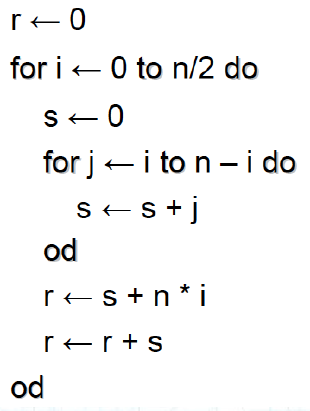
\includegraphics[scale=0.5]{images/okalk_algo.png}
	
	\begin{itemize}
		\pitem Wie oft wird die innere Schleife durchlaufen? \pause $n-2i+1$ mal.
		\pitem Wie kommen wir jetzt auf die Gesamtlaufzeit?
		\pitem $\sum\limits_{i=0}^{n/2} (n-2i+1) \ip = \frac{n}{2}n -2\sum\limits_{i=0}^{n/2}i+\frac{n}{2} \ip = \frac{n^2}{2}+\frac{n}{2}-2\frac{\frac{n}{2}\cdot \left(\frac{n}{2}+1\right)}{2} \ip = \frac{n^2}{2}+\frac{n}{2}-\frac{n^2}{4}-\frac{n}{2}\ip = \frac{1}{4}n^2$
	\end{itemize}
\end{frame}


\subsection{Mastertheorem}

\begin{frame}{Mastertheorem}
	\begin{block}{Formel für Mastertheorem}
		Rekursive Komplexitätsformeln der Form\\
		
		\vspace{.2cm}
		$\quad T(n) = a \cdot T(\frac{n}{b}) + f(n)$
		\vspace{.2cm}
		
		lassen sich mit dem Mastertheorem Komplexitätsklassen zuordnen.
	\end{block}

	\begin{block}{Auflösung des Mastertheorem}
		\begin{description}
			\item[Fall 1:] Wenn $f \in \okalk(n^{\log_b a -\epsilon})$ für ein
			$\epsilon>0$ ist, dann ist $T\in \Theta(n^{\log_b a})$.
			\item[Fall 2:] Wenn $f \in \Theta(n^{\log_b a})$ ist, dann ist
			$T\in \Theta(n^{\log_b a}\log n)$.
			\item[Fall 3:] Wenn $f \in \Omega(n^{\log_b a +\epsilon})$ für ein
			$\epsilon>0$ ist, und wenn es eine Konstante $d$ gibt mit $0<d<1$, so
			dass für alle hinreichend großen $n$ gilt $af(n/b)\leq d f$, dann
			ist $T\in \Theta(f)$.
		\end{description}
	\end{block}
\end{frame}

\begin{frame}{Aufgaben zum Mastertheorem}
	\begin{itemize}
		\pitem $T(n) := 2 T(\frac{n}{4}) + \sqrt{n}$\pause, also $a=2, b=4, f(n) = \sqrt{n}$\pause, also zweiter Fall des Mastertheorems\pause. $T \in \Theta (\sqrt{n}\log n)$
		\pitem $T(n) := 3 T(\frac{n}{2}) + n\log n$\pause, also $a = 3, b=2, f(n) = n\log n$\pause, also erster Fall des Mastertheorems\pause, $T \in \Theta(n^{\log_2 3})$
		\pitem $T(n) := 4 T(\frac{n}{2}) + n^2\sqrt{n}$\pause, also $a = 4, b=2, f(n) = n^2\sqrt{n}$\pause, also dritter Fall des Mastertheorems\pause, $T \in \Theta(n^2\sqrt{n})$.
	\end{itemize}
\end{frame}

\begin{frame}{Aufgaben zum Mastertheorem}
\begin{itemize}
	\item $T(n)=2T(\frac{n}{2})+10n$
	\item $T(n)=20n^2+8T(\frac{n}{2})$
	\item $T(n)=4T(\frac{n}{4})+n^2$
\end{itemize}
\end{frame}

%\subsection{Beweisaufgaben}

%\begin{frame}{Beweisaufgabe zu O-Kalkül}
%	\begin{taskblock}{Beweisaufgabe}
%		Zeige, dass gilt: $3n^3 \not\in \okalk(n^2)$.
%	\end{taskblock}
%
%	\pause
%	
%	Annahme: \ip $3n^3 \in \okalk(n^2)$. 
%	
%	\ip Dann gilt: $\exists c \in \R_+ : \exists n_0 \in \N_0 : \forall n \geq n_0 : \ip c\cdot 3n^3 \leq n^2$.
%	
%	\ip Da der linke Term möglichst klein sein soll\ip, können wir $c < 1$ setzen. \ip Sei $k_0 = \%lceil c \rceil ^{-1} \geq c^{-1}$.
%	
%	\ip Dann: $c \cdot 4k_0^3 = c \cdot k_0 \cdot 3k_0^2 \ip = 3m \cdot k_0^2 \ip \geq k_0^2$ \ip ($m$ durch den Rundungsrest).
%	
%	\ip $m > 1$ und $\forall k \in \N_0, k \geq k_0 : 3k^3 > k^2$.
%\end{frame}


%\section{Automaten}
%
%\begin{frame}{Definition eines endlichen Automaten}
%	\begin{block}{Endlicher Automat}
%		Ein endlicher Automat ist ein Tupel $A = (Z, z_0, X, f, Y, g)$ mit...
%		
%		\begin{itemize}
%			\pitem endliche Zustandsmenge $Z$
%			\pitem Anfangszustand $z_0 \in Z$
%			\pitem Eingabealphabet $X$
%			\pitem Zustandsübergangsfunktion $f: Z \times X \rightarrow Z$
%			\pitem Ausgabealphabet $Y$
%			\pitem Ausgabefunktion 
%			\begin{itemize}
%				\pitem Mealy-Automat: $g: Z \times X \rightarrow Y^*$
%				\pitem Moore-Automat: $h: Z \rightarrow Y^*$
%			\end{itemize}
%		\end{itemize}
%	\end{block}
%\end{frame}


\begin{frame}
	\includegraphics[width=\linewidth]{../images/thatsall.png}
\end{frame}


\end{document}
\def\tutdate{01.02.2018}

\documentclass[handout]{beamer}
\usepackage{../templates/beamerthemekit}
%\usepackage{enumitem}

\usepackage[utf8]{inputenc}
\usepackage[T1]{fontenc}
\usepackage[ngerman]{babel}
\usepackage{listings}
\usepackage{hyperref}
\usepackage{graphicx}

\usepackage{amsmath}
\usepackage{amsthm}
\usepackage{amssymb}
\usepackage{polynom}

%\usepackage{ifthen}
%\usepackage{adjustbox} % for \adjincludegraphics

%\usepackage{tikz}
\usepackage{listings}

%\usepackage[]{algorithm2e}

%\usepackage{colortbl}
\usepackage{verbatim}
%\usepackage{alltt}
%\usepackage{changes}

%\usepackage{pdfpages}
%\usepackage{tabularx}

%\usepackage{euler}


\newcommand{\markBlue}[1]{\textcolor{kit-blue100}{#1}}
\newcommand{\markGreen}[1]{\textcolor{kit-green100}{#1}}
\newcommand{\vertspace}{\vspace{.2cm}}

%\newcommand{\#}{\markBlue{#1}}

%\newcommand{\pitem}{\pause\item}
\newcommand{\p}{\pause}

% -- MATH MACROS
\newcommand{\thistheoremname}{}
\newcommand{\G}{\mathbb{Z}}
\newcommand{\B}{\mathbb{B}}
\newcommand{\R}{\mathbb{R}}
\newcommand{\N}{\mathbb{N}}
\newcommand{\Q}{\mathbb{Q}}
\newcommand{\C}{\mathbb{C}}
\newcommand{\Z}{\mathbb{Z}}
\newcommand{\F}{\mathbb{F}}
\newcommand{\mi}{\mathrm{i}}
\renewcommand{\epsilon}{\varepsilon}
\newcommand{\okalk}{\mathscr{O}}


\newenvironment<>{taskblock}[1]{%
	\setbeamercolor{block title}{fg=kit-orange15,bg=kit-orange100}
	\setbeamercolor{block body}{fg=black,bg=kit-orange30}%
	\begin{block}#2{#1}}{\end{block}}

\setbeamertemplate{enumerate items}[default]

% Aussagenlogik Symbole
\newcommand{\W}{w}
\renewcommand{\F}{f}

% Kodierung
\newcommand{\frepr}{\textbf{repr}}
\newcommand{\fRepr}{\textbf{Repr}}
\newcommand{\fZkpl}{\textbf{Zkpl}}
\newcommand{\fbin}{\textbf{bin}}
\newcommand{\fdiv}{\textbf{ div }}
\newcommand{\fmod}{\textbf{ mod }}

% Speicherabbild
\newenvironment{memory}{\begin{tabular}{r | l}Adresse&Wert\\\hline\hline}{\end{tabular}}
\newcommand{\memrow}[2]{#1 & #2 \\\hline}

% Praedikatenlogik
\newcommand{\objequiv}{\stackrel{\cdot}{=}}
\newcommand{\pval}{val_{D,I,\beta}}

% Neue Befehle
\newcommand{\ip}{\pause} % inline pause, für mitten im satz
\newcommand{\pitem}{\pause\item} % für aufzählungen
\newcommand{\bp}{\pause} % block pause, für zwischen blöcken
\title[Grundbegriffe der Informatik]{ICPC\\Gruppe 2}
\date{\tutdate}
\subtitle{\tutTitle}
\author{Elias Schaut, Dennis Kobert, Niklas Kniep, Lam Vo, Ilia Bozhinov}

\institute{}

\titleimage{bg}
%\titleimage{bg-advent}

%
\ifthenelse{\equal{\compiletype}{livebeamer}}
	{
		\def\livebeamermode{1}
	}{}

\ifthenelse{\equal{\compiletype}{print}}
	{
		\def\printmode{1}
	}{}

\setbeamercovered{invisible}

%\usepackage[citestyle=authoryear,bibstyle=numeric,hyperref,backend=biber]{biblatex}
%\addbibresource{templates/example.bib}
%\bibhang1em

	
\def\tutTitle{Automaten und reguläre Sprachen}
\begin{document}

\selectlanguage{ngerman}

%title page
\begin{frame}
	\titlepage
\end{frame}

\section{Automaten}
\subsection{Mealy-Automat}
\begin{frame}{Mealy-Automat}
	\begin{block}{Mealy-Automat}
		Ein Mealy-Automat ist ein Tupel $A = (Z, z_0, X, f, Y, h)$ mit...
		\begin{itemize}
			\pitem $Z$ endliche, nichtleere Zustandsmenge 
			\pitem $z_0 \in Z$ Startzustand 
			\pitem $X$ Eingabealphabet 
			\pitem $f: Z \times X \rightarrow Z$ Zustandsübergangsfunktion 
			\pitem $Y$ Ausgabealphabet 
			\pitem $h: Z \times X \rightarrow Y^*$ Ausgabefunktion 
		\end{itemize}
	\end{block}

	\pause 
	
	
	\textbf{Darstellung als Graph}\\
	\begin{itemize}
		\pitem Zustände $\rightarrow$ Knoten
		\pitem Startzustand $\rightarrow$ Pfeil an diesen Knoten (nicht vergessen!)
		\pitem Zustandsüberführungsfunktion $\rightarrow$ Kanten mit Beschriftung \(w \in X\)
		\pitem Ausgabefunktion $\rightarrow$ zusätzliche Kantenbeschriftung \(w \in Y^*\)
	\end{itemize}
\end{frame}

\begin{frame}{Beispiel Mealy-Automat}
	\includegraphics[scale=0.6]{images/MealyBsp.png}
\end{frame}

\begin{frame}{Mealy-Automat}
	\includegraphics[scale=0.25]{images/MealyEnd.png}
\end{frame}

\begin{frame}{Mealy-Automat}
	\includegraphics[scale=0.25]{images/MealyEndKonkat.png}
\end{frame}

\begin{frame}{Mealy-Automat}
	\includegraphics[scale=0.25]{images/MealyOut.png}
\end{frame}

\begin{frame}{Mealy-Automat}
	\includegraphics[scale=0.25]{images/MealyOutKonkat.png}
\end{frame}

\begin{frame}{Beispiel Mealy-Automat}
	\includegraphics[scale=0.5]{images/MealyBsp.png}
	%\includegraphics[scale=0.25]{images/MealyBspFunk.png}
	\begin{itemize}
		\item<1|only@1>[] {
			\begin{itemize}
				\item \(f_* (A, aabba) = D\)
				\item \(f_{**} (A, aabba) = ABBCCD\)
				\item \(g_* (A, aabba) = x\)
				\item \(g_{**} (A, aabba) = 1010x\)		
			\end{itemize}
		}
		\item<2-3|only@2-3>[] {
			\begin{itemize}
				\item[] Für welche \(w \in X^*\) gilt \(f_* (A, w) \neq D\)? \pause \pause
				\item[] Für genau alle \(w \in \{a\}^* \{b\}^*\).
			\end{itemize}
		}
		\item<4-5|only@4-5>[] {
			\begin{itemize}
				\item[] Für welche \(w \in X^*\) gilt \(g_* (A, w) = 0\)? \pause \pause
				\item[] Für genau alle \(w \in \{a\}^* \cdot \{b\} \cdot \{b\}^+ \cup \{a\} \cdot \{a\}^+\).
			\end{itemize}
		}
	\end{itemize}
\end{frame}

\subsection{Moore-Automat}

\begin{frame}{Moore-Automat}
	\begin{block}{Moore-Automat}
		Ein Moore-Automat ist ein Tupel $A = (Z, z_0, X, f, Y, h)$ mit...
		\begin{itemize}
			\item $Z$ endliche Zustandsmenge 
			\item $z_0 \in Z$ Anfangszustand 
			\item $X$ Eingabealphabet 
			\item $f: Z \times X \rightarrow Z$ Zustandsübergangsfunktion 
			\item $Y$ Ausgabealphabet 
			\pitem[$\rightarrow$] \textcolor{red}{Bis hierhin alles wie bei Mealy!}
			\pitem $h: Z \rightarrow Y^*$ Ausgabefunktion 
		\end{itemize}
	\end{block}

	\pause

	\begin{itemize}
		\pitem Zustände $\rightarrow$ Knoten
		\pitem Startzustand $\rightarrow$ Pfeil an diesen Knoten (nicht vergessen!)
		\pitem Zustandsüberführungsfunktion $\rightarrow$ Kanten mit Beschriftung \(w \in X\)
		\pitem Ausgabefunktion $\rightarrow$ zusätzliche Knotenbeschriftung \(w \in Y^*\)
	\end{itemize}
\end{frame}

\begin{frame}{Funktionen}
	\begin{itemize}
		\item \(f_*\) und \(f_{**}\) wie beim Mealy-Automaten
		\item \(g_* := h \circ f_*\)
		\item \(g_{**} := h_{**} \circ f_{**}\)
		Dabei bezeichnet \(h_{**}\) den durch \(h\) induzierten Homomorphismus.
	\end{itemize}
\end{frame}

\begin{frame}{Beispiel}
	\includegraphics[scale=0.3]{images/Moore.png}
	\begin{itemize}
		\item<1|only@1>[] {
			\begin{itemize}
				\item \(f_* (A, aabba) = D\)
				\item \(f_{**} (A, aabba) = ABACCD\)
				\item \(g_* (A, aabba) = x\)
				\item \(g_{**} (A, aabba) = 11100x\)		
			\end{itemize}
		}
		\item<2-3|only@2-3>[] {
			\begin{itemize}
				\item[] Wann gilt \(g_* (A, w) = 0\)? \pause \pause
				\item[] Genau dann, wenn \(w \in \{aa\}^* \{b\}^+\).
			\end{itemize}
		}
	\end{itemize}
\end{frame}

\begin{frame}{Umwandlung}
	\textbf{Bemerkung}\\
	Für jeden Mealy-Automaten kann man einen Moore-Automaten konstruieren, der genau die gleiche Aufgabe erfüllt, und umgekehrt.
\end{frame}

%Mal selber ausprobieren lassen
\begin{frame}{Umwandlung Mealy- in Moore-Automat}
	Links ein Mealy-, rechts ein Moore-Automat
	
	
	\begin{figure}[!tbp]
		\centering
		\begin{minipage}[b]{0.4\textwidth}
			\includegraphics[width=\textwidth]{images/MealyBsp.png}
			\caption{Mealy}
		\end{minipage}
		\hfill
		\pause
		\begin{minipage}[b]{0.4\textwidth}
			\includegraphics[width=\textwidth]{images/MooreBsp.png}
			\caption{Moore}
		\end{minipage}
	\end{figure}

\end{frame}

\subsection{Endliche Akzeptoren}
\begin{frame}{Endliche Akzeptoren}
	\begin{itemize}
		\pitem Sonderfall von Moore-Automaten
		\pitem Bei einem Akzeptor will man nur wissen, ob die Eingabe akzeptiert wurde oder nicht (also reicht ein Bit als Ausgabealphabet)
		\pitem Statt der Ausgabefunktion $h$ schreibt man einfach die Menge der akzeptierenden Zustände $F \subseteq Z$ auf
		\pitem Zustände, die nicht akzeptieren, heißen ablehnend
		\pitem Im Graphen werden akzeptierende Zustände einfach mit einem doppelten Kringel gekennzeichnet \includegraphics[scale=0.6]{images/Doppelkringel.png}
	\end{itemize}
\end{frame}

\begin{frame}{Akzeptierte Wörter und Sprachen}
	
	\begin{block}{Akzeptierte Wörter}
		Ein Wort $w \in X^*$ wird vom endlichen Akzeptor akzeptiert, wenn man ausgehend vom Anfangszustand bei Eingabe von w in einem akzeptierenden Zustand endet.
	\end{block}

	\pause
	
	\textbf{Bemerkung}\\
	\begin{itemize}
		\item Wird ein Wort nicht akzeptiert, dann wurde es abgelehnt
	\end{itemize}

	\pause
	
	\begin{block}{Akzeptierte formale Sprache}
		Die von einem Akzeptor $A$ akzeptierte formale Sprache $L(A)$ ist die Menge aller von ihm akzeptierten Wörter.
	\end{block}
\end{frame}

\begin{frame}{Endliche Akzeptoren}
	\begin{taskblock}{Aufgabe zu endlichen Akzeptoren}
		Konstruiere einen endlichen Akzeptor, der die Sprache $L_1(A) = \{w \in \{a,b\}^* : (N_a(w) \geq 3 \land N_b(w) \geq(2)\}$ erkennt.
	\end{taskblock}
	
	\pause
	\textbf{Lösung}\\
	\includegraphics[scale=0.6]{images/AufgAkzeptor2.png}
\end{frame}
		
		

\begin{frame}{Endliche Akzeptoren}
	\begin{taskblock}{Aufgabe zu endlichen Akzeptoren}
		Konstruiere einen endlichen Akzeptor, der die Sprache $L_2(A) = \{w_1 ababb w_2| w_1, w_2 \in \{a,b\}^*\}$ erkennt.
	\end{taskblock}
	
	\pause
	\textbf{Lösung}\\
	\includegraphics[scale=0.7]{images/AufgAkzeptor.png}\\
	\pause
	\begin{taskblock}{Aufgabe}
		Konstuiere einen endlichen Akzeptor der die Sprache $L_3 =\{w \in \{a,b\}^*| w \not \in L_2\}$ akzeptiert.
	\end{taskblock}
	\pause
	\textbf{Lösung} \\Ablehnende Zustände wereden zu akzeptierenden und andersrum.
\end{frame}		 

\begin{frame}{Endliche Akzeptoren}
	\begin{taskblock}{Aufgaben zu endlichen Akzeptoren}
		\begin{itemize}
			\item Gebe für den unten stehenden Automaten an, welche Sprache dieser akzeptiert.
			\item Gebe für die folgende Sprache über dem Alphabet $\{a,b\}$ einen endlichen Akzeptor an:
			$L = \{w \in \Sigma^* | N_a(w) \text{ mod } 3 > N_b(w) \text{ mod } 2\}$
		\end{itemize}
	\end{taskblock}

	\includegraphics[scale=0.7]{images/AufgAkzeptor1.png}
\end{frame}

\begin{frame}{Lösungen}	
	\textbf{Lösung 1}\\
	$L = \{w \in \Sigma^* | |w| \text{ mod } 2 = 1\}$ (Worte ungerader Länger)\\
	\pause
	\textbf{Lösung 2}\\
	\includegraphics[scale=0.8]{images/LoesAkzeptor.png}
\end{frame}

\begin{frame}{Endliche Akzeptoren}
	Wann wird das leere Wort $\varepsilon$ von einem endlichen Akzeptor akzeptiert?\\
	\pause
	$\varepsilon \in L(A)$ gilt genau dann, wenn der Startzustand akzeptiert wird.
\end{frame}

\begin{frame}
Gibt es einen endlichen Akzeptor, der die Sprache $L_1=\{w \in \{1\}^*|$w ist Teilwort der Binärdarstellung von $ \pi\}$ erkennt \newline \pause
Gibt es einen endlichen Akzeptor, der die Sprache $L_2=\{0^k1^k|k\in \N_0\}$ erkennt
\end{frame}

\section{Turingmaschinen}

\begin{frame}{Turingmaschinen}
Was sind Turingmaschinen?

\begin{itemize}
	\pitem Sehr mächtige Erweiterung Automat
	\begin{itemize}
		\pitem Was heißt mächtig?
		\pitem Turingmaschinen können eine große Vielfalt von Problemen lösen, einschließlich vieler in GBI besprochener Probleme
	\end{itemize}
	\pitem Gesteuert durch einen endlichen Automaten\ip, aber mit einem \markBlue{unendlichen Arbeitsband} zum Zwischenspeichern von Informationen
	\pitem Besitzen einen Kopf um auf dem Band zu lesen und zu schreiben
	\pitem Turingmaschinen sind sozusagen genauso mächtig wie Computer
	\begin{itemize}
		\pitem können also benutzt werden, um für Probleme zu entscheiden, \markGreen{ob sie gelöst werden können oder nicht}
	\end{itemize}
\end{itemize}
\end{frame}

\begin{frame}{Definition von Turingmaschinen}
\begin{block}{Definition von Turingmaschinen}
Eine Turingmaschine $T = (Z, z_0, X, f, g, m)$ besteht aus:
\begin{itemize}
	\pitem $Z$ Zustandsmenge
	\pitem $z_0 \in Z$ Startzustand
	\pitem $X$ Bandalphabet
	\pitem $\Box$ Blanksymbol (sozusagen Markierung für Leerzeichen)
	\pitem $f: Z \times X \rightarrow Z$ partielle Zustandsübergangsfunktion
	\pitem $g: Z \times X \rightarrow X$ partielle Ausgabefunktion
	\pitem $m: Z \times X \rightarrow \{L, N, R\}$ partielle Bewegungsfunktion
\end{itemize}
\end{block}

Anmerkung: partielle Funktionen sind \markGreen{nicht linkstotal}, also manche Elemente des Definitionsbereichs werden nicht abgebildet.
\end{frame}

\begin{frame}{Beispiel einer Turingmaschine}
\includegraphics[scale=0.5]{images/turingexample_withoutannotations.png}
\end{frame}

\begin{frame}{Beispiel einer Turingmaschine}
\includegraphics[scale=0.5]{images/turingexample_withannotations.png}
\end{frame}

\begin{frame}{Funktionen von Turingmaschinen}
\includegraphics[scale=0.4]{images/turingexample_smallspacing.png}

Wie sehen die konkreten Abbildungsvorschriften der linken vier Pfeile aus?

\begin{columns}
\begin{column}{0.3\textwidth}

\vspace{.2cm}

% vielleicht an die tafel schreiben was die funktionen vom namen her machen (f: zustandsübergang), hat so nicht mehr auf die folie gepasst
\begin{itemize}
\item $f: Z \times X \rightarrow Z$
\item $g: Z \times X \rightarrow X$
\item $m: Z \times X \rightarrow \{L, N, R\}$
\end{itemize}
\end{column}

\begin{column}{0.7\textwidth}
\begin{tabular}{r || c | c | c}
& f & g & m\\\hline\hline

%erste Zeile als Beispiel
$0|0,N$ & $(s1, 0) \mapsto s6$ & $(s1, 0) \mapsto 0$ & $(s1, 0) \mapsto N$ \\\hline

\pause $1|0, R$ 
\pause & $(s1, 1) \mapsto s2$
\pause & $(s1, 1) \mapsto 0$
\pause & $(s1, 1) \mapsto R$ \\\hline

\pause $1|1, R$ 
\pause & $(s2, 1) \mapsto s2$
\pause & $(s2, 1) \mapsto 1$
\pause & $(s2, 1) \mapsto R$ \\\hline

\pause $0|0, R$ 
\pause & $(s2, 1) \mapsto s3$
\pause & $(s2, 1) \mapsto 0$
\pause & $(s2, 1) \mapsto R$ \\\hline

\end{tabular}
\end{column}
\end{columns}

\end{frame}


\begin{frame}{Das Band einer Turingmaschine}
\begin{itemize}
\pitem Unendliche Anreihung von Zeichen, die nach links und rechts unbegrenzt weiter geht

\p\includegraphics[scale=0.3]{images/turing_band.png}

\pitem Die Turingmaschine hat einen Kopf, mit dem sie das aktuelle Zeichen lesen oder überschreiben kann, oder kann ihn nach links oder rechts bewegen.

\pitem Das Band einer Turingmaschine wird benutzt als...
\begin{itemize}
\pitem Erhalten der Eingabe: \ip Bevor die Turingmaschine startet, steht das Eingabewort auf dem Band, der Kopf steht auf dem ersten Zeichen der Eingabe.
\pitem Rückgabe der Ausgabe: \ip Nach Beenden steht auf dem Band die Ausgabe (und der Kopf irgendwo).
\pitem Zwischenspeicher: \ip Die Turingmaschine kann überall Informationen zwischenspeichern, diese müssen von der TM am Ende aber gelöscht werden.
\end{itemize}
\end{itemize}
\end{frame}

% Am besten erst mal die aufgaben zusammen durchrechnen
\begin{frame}{Beispielabarbeitungen}
\begin{columns}
\begin{column}{0.5\textwidth}
\begin{taskblock}{Gemeinsame Übung}
Arbeite folgende Wörter mit der Turingmaschine ab:
\begin{itemize}
\item $0$
\item $1$
\item $11$
\item $111$
\end{itemize}
Was macht die Turingmaschine?
\end{taskblock}
\end{column}

\begin{column}{0.5\textwidth}
\includegraphics[scale=0.4]{images/turingmaschine_1k.png}
\end{column}
\end{columns}
\end{frame}


\begin{frame}
	\includegraphics[width=\linewidth]{../images/thatsall.png}
\end{frame}


\end{document}
\def\tutdate{30.10.2019}

\documentclass[handout]{beamer}
\usepackage{../templates/beamerthemekit}
%\usepackage{enumitem}

\usepackage[utf8]{inputenc}
\usepackage[T1]{fontenc}
\usepackage[ngerman]{babel}
\usepackage{listings}
\usepackage{hyperref}
\usepackage{graphicx}

\usepackage{amsmath}
\usepackage{amsthm}
\usepackage{amssymb}
\usepackage{polynom}

%\usepackage{ifthen}
%\usepackage{adjustbox} % for \adjincludegraphics

%\usepackage{tikz}
\usepackage{listings}

%\usepackage[]{algorithm2e}

%\usepackage{colortbl}
\usepackage{verbatim}
%\usepackage{alltt}
%\usepackage{changes}

%\usepackage{pdfpages}
%\usepackage{tabularx}

%\usepackage{euler}


\newcommand{\markBlue}[1]{\textcolor{kit-blue100}{#1}}
\newcommand{\markGreen}[1]{\textcolor{kit-green100}{#1}}
\newcommand{\vertspace}{\vspace{.2cm}}

%\newcommand{\#}{\markBlue{#1}}

%\newcommand{\pitem}{\pause\item}
\newcommand{\p}{\pause}

% -- MATH MACROS
\newcommand{\thistheoremname}{}
\newcommand{\G}{\mathbb{Z}}
\newcommand{\B}{\mathbb{B}}
\newcommand{\R}{\mathbb{R}}
\newcommand{\N}{\mathbb{N}}
\newcommand{\Q}{\mathbb{Q}}
\newcommand{\C}{\mathbb{C}}
\newcommand{\Z}{\mathbb{Z}}
\newcommand{\F}{\mathbb{F}}
\newcommand{\mi}{\mathrm{i}}
\renewcommand{\epsilon}{\varepsilon}
\newcommand{\okalk}{\mathscr{O}}


\newenvironment<>{taskblock}[1]{%
	\setbeamercolor{block title}{fg=kit-orange15,bg=kit-orange100}
	\setbeamercolor{block body}{fg=black,bg=kit-orange30}%
	\begin{block}#2{#1}}{\end{block}}

\setbeamertemplate{enumerate items}[default]

% Aussagenlogik Symbole
\newcommand{\W}{w}
\renewcommand{\F}{f}

% Kodierung
\newcommand{\frepr}{\textbf{repr}}
\newcommand{\fRepr}{\textbf{Repr}}
\newcommand{\fZkpl}{\textbf{Zkpl}}
\newcommand{\fbin}{\textbf{bin}}
\newcommand{\fdiv}{\textbf{ div }}
\newcommand{\fmod}{\textbf{ mod }}

% Speicherabbild
\newenvironment{memory}{\begin{tabular}{r | l}Adresse&Wert\\\hline\hline}{\end{tabular}}
\newcommand{\memrow}[2]{#1 & #2 \\\hline}

% Praedikatenlogik
\newcommand{\objequiv}{\stackrel{\cdot}{=}}
\newcommand{\pval}{val_{D,I,\beta}}

% Neue Befehle
\newcommand{\ip}{\pause} % inline pause, für mitten im satz
\newcommand{\pitem}{\pause\item} % für aufzählungen
\newcommand{\bp}{\pause} % block pause, für zwischen blöcken
\title[Grundbegriffe der Informatik]{ICPC\\Gruppe 2}
\date{\tutdate}
\subtitle{\tutTitle}
\author{Elias Schaut, Dennis Kobert, Niklas Kniep, Lam Vo, Ilia Bozhinov}

\institute{}

\titleimage{bg}
%\titleimage{bg-advent}

%
\ifthenelse{\equal{\compiletype}{livebeamer}}
	{
		\def\livebeamermode{1}
	}{}

\ifthenelse{\equal{\compiletype}{print}}
	{
		\def\printmode{1}
	}{}

\setbeamercovered{invisible}

%\usepackage[citestyle=authoryear,bibstyle=numeric,hyperref,backend=biber]{biblatex}
%\addbibresource{templates/example.bib}
%\bibhang1em

	
\def\tutTitle{Wörter und Formale Sprachen}
\begin{document}

\selectlanguage{ngerman}

%title page
\begin{frame}
	\titlepage
\end{frame}

\section{Hinweise}

\begin{frame}{Hinweise zur Abgabe}
	\begin{itemize}
		\item Blätter vollständig nutzen, nicht ein Blatt pro Aufgabe
		\item Aufgabenblatt nicht mit abgeben
		\item Nur antworten, was gefragt wurde (keine falschen oder nicht gefragten Lösungswege)
		\item "`geben Sie an"' erfordert keinen Beweis
		\item Lieber sprachlich erklären, wenn man Probleme mit formalen Beweisen hat (falls nicht explizit einer gefordert ist)
		\item Genau schreiben, warum die Behauptung aus dem folgt, was ihr gerade bewiesen habt
		\item Unterscheidet Element und Teilmenge: $x \in A$ oder $\{x\} \subset A$
		\item Vereinigung ist $\cup$ und nicht $+$
	\end{itemize}
\end{frame}

\begin{frame}{Typische Fehler}
	\begin{itemize}
		\item Sprachlich: A oder B ist die leere Menge
		\item Formal: $A = \emptyset \lor B = \emptyset$ Nicht: \sout{$A \lor B = \emptyset$}
		\item Leere Menge ist $\emptyset $ oder $\{\}$, nicht 0
	\end{itemize}
\end{frame}

\section{Mengen}

\begin{frame}{Mengen}
	Seien $A=\{1,2,3,4\}, B=\{3,4,5,6,7\}, C=\{5,6,7\}$. Bestimme
	\begin{itemize}
		\item $A \cup B$
		\item $A \cup C$
		\item $A \cap B$
		\item $A \cap C$
	\end{itemize}
	sowie die Kardinalität dieser Mengen.
\end{frame}
\begin{frame}{Mengen}
	Lösung:
	\begin{itemize}
		\item $A \cup B = \{1,2,3,4,5,6,7,\}$ und $\mid A \cup B\mid = 7$
		\pause
		\item $A \cup B = \{1,2,3,4,5,6,7,\}$ und $\mid A \cup C\mid = 7$
		\pause
		\item $A \cap B = \{3,4\}$ und $\mid A \cap B \mid = 2$
		\pause
		\item $A \cap C = \emptyset$ und $\mid\emptyset\mid = 0$
	\end{itemize}
\end{frame}

\begin{frame}{Mengen}
	\begin{block}{Aufgabe aus WS16/17}
		Es seinen A,B und C Mengen. Beweisen oder widerlegen Sie:
		$A \backslash (B \backslash C) = (A \backslash B)\backslash C$
	\end{block}
\end{frame}
\begin{frame}{Mengen}
	\begin{block}{Aufgabe aus WS16/17}
		Es seinen A,B und C Mengen. Beweisen oder widerlegen Sie:
		$A \backslash (B \backslash C) = (A \backslash B)\backslash C$
	\end{block}
	\begin{block}{Widerlegung durch Gegenbeispiel}
		Seien $A = \{1,2,3\}, B = \{3,4,5\}$ und $C = \{3\}$.
		Dann ist $\{1,2,3\} \backslash (\{3,4,5\} \backslash \{3\}) = \{1,2,3\} \backslash \{4,5\} = \{1,2,3\} \neq$
		$\{1,2\} = \{1,2\} \backslash \{3\} = (\{1,2,3\} \backslash \{3,4,5\}) \backslash \{3\}$
	\end{block}
\end{frame}
\begin{frame}{Mengenäquivalenz}
	\begin{block}{Zeigen Sie}
		$A \cup (B \cap C) = (A \cup B) \cap (A \cup C)$
		\begin{itemize}
			\pause\item ``$\subseteq$'': Sei $x \in A \cup (B\cap C).$ Dann ist $x \in A$ oder $x \in (B \cap C)$
			\begin{itemize}
				\pause
				\item Falls $x\in A$, dann gilt auch $x\in (A\cup B)$ und $x\in (A\cup C)$. Also
				insbesondere $x\in(A\cup B)\cap(A\cup C)$.
				\pause
				\item Falls $x\in(B\cap C)$, dann gilt auch $x\in (A\cup B)$ und $x\in (B\cup C)$. Also
				insbesondere $x\in(A\cup B)\cap(A\cup C)$.
				\pause
			\end{itemize}
			\item ``$\supseteq$'': $x\in(A\cup B)\cap(A\cup C)$. Dann liegt x in $(A\cup B)$ und $(A\cup C)$.
			Also liegt x in A oder in (B und C). Folglich gilt 
			$x\in A\cup(B\cap C)$.
			\pause\item Insgesamt ist also $A\cup(B\cap C) = (A\cup B)\cap(A\cup C)$.
		\end{itemize}
	\end{block}
\end{frame}

\begin{frame}{Mengen}
	\begin{block}{Aufgabe aus WS16/17}
		Es sei M eine Menge und es seien $A\subseteq M$ und $B\subseteq M$. Beweisen Sie:
		$M\backslash(A\cap B) = (M\backslash A)\cup(M\backslash B)$
		\begin{itemize}
			\pause \item ``$\subseteq$'': Sei $x\in M\backslash(A\cap B)$. Dann ist $x\in M$ und $x\notin A$ oder $x\notin B$.
			\\Somit ist
			\begin{itemize}
				\item $x\in M$ und $x\notin A$ oder
				\item $x\in M$ und $x\notin B$.
			\end{itemize}
			Also ist $x\in(M\backslash A)$ oder $(M\backslash B)$, folglich also
			$x\in(M\backslash A)\cup(M\backslash B)$.

			\pause\item ``$\supseteq$'': Sei $x\in(M\backslash A)\cup(M\backslash B)$. Dann ist $x\in(M\backslash A)$ oder\\
			$x\in(M\backslash B)$. Somit ist
			\begin{itemize}
				\item $x\in M$ und $x\notin A$ oder
				\item $x\in M$ und $x\notin B$.
			\end{itemize}
			Also ist $x\in M$, und $x\notin A$ oder $x\notin B$. Dann ist $x\in M$ und \\
			$x\notin(A\cap B)$, folglich also $x\in M\backslash(A\cap B)$.
		\end{itemize}
	\end{block}
\end{frame}

\section{Wörter}

\begin{frame}{Wörter}
	\begin{block}{Konkatenation}
		Durch Konkatenation werden einzelne Buchstaben aus einem Alphabet miteinander verbunden.
	\end{block}

	\begin{itemize}
		\pitem Symbol: $\cdot$\pause , also zwei Buchstaben $a$ und $b$ miteinander konkateniert: $a \cdot b$.
		\pitem Nicht kommutativ : $a \cdot b \neq b \cdot a$
		\pitem Aber assoziativ : $(a \cdot b) \cdot c = a \cdot (b \cdot c)$
		\pitem Kurzschreibweise : Ohne Punkte , also $a \cdot b = ab$
	\end{itemize}
\end{frame}

\begin{frame}{Wörter}
	\begin{block}{Wörter: Intuitivere Definition}
		Ein Wort $w$ entsteht durch die Konkatenation durch Buchstaben aus einem Alphabet.
	\end{block}

	$\rightarrow$ Also Abfolge von Zeichen über ein Alphabet A.

	\pause Sei $A := \{a, b, c\}$.

	\begin{itemize}
		\pitem Mögliche Worte: \pause $w_1 := a \cdot b$\pause , $w_2 = b \cdot c \cdot c$\pause , $w_3 = a \cdot c \cdot c \cdot b \cdot a$.
		\pitem Keine möglichen Worte: \pause $d$.
		\end{itemize}
\end{frame}

\begin{frame}{Wörter}
	\begin{block}{Wörter: Abstraktere Definition}
		Ein Wort $w$  über dem Alphabet $A$  ist definiert als surjektive Abbildung  $w : \Z_n \rightarrow A$. Dabei heißt $n$ die Länge $|w|$ des Wortes.
	\end{block}

	\begin{itemize}
		\pitem $\Z_n$  $ = \{i \in \N : 0 \leq i < n \}$
		
		\pause $\Z_3  = \{0, 1, 2\},  \Z_2 = \{0, 1\}, \Z_0 = \emptyset$.
		
		\pitem Länge oder Kardinalität eines Wortes:  $|w|$. \pause $|abcde|$ $= 5$.
		
		\pitem Wort $w = abdec$ als Relation aufgeschrieben: \pause $w = \{(0, a), (1, b), (2, d), (3, e), (4, c)\}$.  Also $w(0) = a, w(1) = b, w(2) = d, \dots$
		
		\pause Damit sieht man auch: $|w| = |\{(0, a), (1, b), (2, d), (3, e), (4, c)\}| = 5$.
	\end{itemize}
\end{frame}

\begin{frame}{Wörter}
	\begin{itemize}
		\item Wort der Kardinalität 0?
	\end{itemize}

	\pause

	\begin{block}{Das leere Wort}
		Das leere Wort $\varepsilon$ ist definiert ein Wort mit Kardinalität 0 , also mit 0 Zeichen.
	\end{block}

	\begin{itemize}
		\pitem Leere Wort wird interpretiert als ``nicht sichtbar'' und kann überall platziert werden\pause : $aabc = a\epsilon abc = \epsilon\epsilon a\epsilon bc \epsilon$.
		\pitem $|\{\epsilon\}|$ \pause $ = 1$ , die Menge ist nicht leer! Das leere Wort ist nicht \emph{nichts}! (Vergleiche leere Menge)
		\pitem $|\epsilon| = 0$.
		\pitem Formale Definition:\pause $\epsilon : \emptyset \rightarrow \emptyset $
	\end{itemize}
\end{frame}

\begin{frame}{Mehr über Wörter}
	\begin{block}{$A^n$}
		Zu einem Alphabet $A$ ist $A^n$ definiert als die Menge aller Wörter der Länge $n$ über dem Alphabet $A$.
	\end{block}

	\begin{itemize}
		\pitem Nicht mit Mengenpotenz verwechseln!
		\pitem $A := \{a, b, c\}$\pause , $A^2 = \{aa, ab, ac, ba, bb, bc, ca, cb, cc\}$. \pause $A^1 = A, \pause A^0 = \{\epsilon\}$.
	\end{itemize}
	
	\pause Die Menge aller Wörter  \emph{beliebiger} Länge: \pause
	\begin{itemize}
		\item $A^* := \bigcup_{i \in \N_0} A_i$
		\pitem $A := \{a, b, c\}$ . $aa \in A^* , abcabcabc \in A^* , aaaa \in A^* , \epsilon \in A^*$.
	\end{itemize}
\end{frame}

\begin{frame}{Mehr über Wörter}
	\begin{block}{Wort Potenzen}
		Sich direkt wiederholende Teilworte kann man als Wortpotenz darstellen , daher $w_i^n = w_i \cdot w_i \cdots w_i$ (n $\times$ mal).
	\end{block}

	\begin{itemize}
		\pitem $a^4 = aaaa$\pause , $b^3 = bbb$\pause , $c^0 = \pause \epsilon$\pause , $d^1 = \pause d$.
		\pitem $a^3c^2b^6 \pause = aaaccbbbbbb$.
		\pitem $b \cdot a \cdot (n \cdot a)^2$ \pause $ = banana$.
		\end{itemize}
\end{frame}

\begin{frame}{Übung zu Wörter}
	Sei $A$ ein Alphabet.
	
	\begin{taskblock}{Übung zu Wörter}
		\begin{enumerate}
			\item Finde Abbildung $f: A^* \rightarrow A^*$, sodass für alle $w \in A^*$ gilt: \\\quad $2 \cdot |w| = |f(w)|$.
			\item Finde Abbildung $g: A^* \rightarrow A^*$, sodass für alle $w \in A^*$ gilt: \\\quad $|w| + 1 = |g(w)|$.
			\item Sind $f, g$ injektiv und/oder surjektiv?
		\end{enumerate}
	\end{taskblock}

	\pause
	
	\begin{enumerate}
		\item $f: A^* \rightarrow A^*, w \mapsto w \cdot w$.
		\pitem $g: A^* \rightarrow A^*, w \mapsto w \cdot x, x \in A$.
	\end{enumerate}
\end{frame}

\begin{frame}{Übung zu Wörter}
	\begin{enumerate}
		\item $f: A^* \rightarrow A^*, w \mapsto w \cdot w$.
		\begin{itemize}
			\pitem $f$ ist injektiv\pause , denn jedes $w$ aus der Bildmenge wird von maximal einem Wort abgebildet.
			\pitem $f$ ist nicht surjektiv\pause , denn z.B. bildet nichts auf $x \in A$ ab (oder auf andere Wörter mit ungerader Anzahl an Buchstaben).
		\end{itemize}
		\pitem $g: A^* \rightarrow A^*, w \mapsto w \cdot x, x \in A$.
		\begin{itemize}
			\pitem $g$ ist injektiv.
			\pitem $g$ ist nicht surjektiv\pause , denn z.B. bildet nichts auf $\epsilon$ ab.
		\end{itemize}
	\end{enumerate}
\end{frame}

\section{Formale Sprachen}

\begin{frame}{Formale Sprache}
	\begin{itemize}
		\pitem Was war nochmal $A^*$? Menge aller Wörter \emph{beliebiger} Länge über Alphabet $A$.
	\end{itemize}

	\pause
	
	\begin{block}{Formale Sprache}
		Eine Formale Sprache $L$ über einem Alphabet $A$ ist eine Teilmenge $L \subseteq A^*$.
	\end{block}

	\begin{itemize}
		\pitem Zufälliges Beispiel: \pause $A := \{b, n, a\}$.
		\begin{itemize}
			\pitem $L_1 := \{ban, baan, nba, aa\}$ ist eine mögliche formale Sprache über $A$.
			\pitem $L_2 := \{banana, bananana, banananana, ...\}$ \pause $ = \{w : w = bana(na)^k, k \in \N\}$ auch.
			\pitem $L_3 := \{ban, baan, baaan, ...\}$ auch. \pause Andere Schreibweise? \pause \\ $ L_3 = \{w : w = ba^kn, k \in \N \}$
		\end{itemize}
		\pitem Formale Sprachen sind also nicht zwangsweise endliche Mengen.
		\pitem Praktischeres Beispiel: $A := \{w : w $ ist ein ASCII Symbol $\}$.
		\pitem $L_4 := \{w : $ w ist korrekt kompilierendes Java-Programm $\}$ 
	\end{itemize}
\end{frame}

\begin{frame}{Übung zu formalen Sprachen}
	$A := \{a, b\}$
	
	\begin{itemize}
		\pitem Sprache $L$ aller Wörter über $A$, die nicht das Teilwort $ab$ enthalten?
		\begin{itemize}
			\pitem Was passiert wenn ein solches Wort ein $a$ enthält? \pause Dann keine $b$'s mehr!
			\pitem $L = \{w_1 \cdot w_2 : w_1 \in \{b\}^*$ und $w_2 \in \{a\}^* \}$
			\pitem Andere Möglichkeit\pause : Suche Wörter mit $ab$ und nehme diese Weg.
			\pitem $L = \{a, b\}^*\pause \backslash\{ w_1 \cdot ab \cdot w_2 : w_1, w_2 \in \{a,b\}^* \}$
		\end{itemize}
	\end{itemize}
\end{frame}

\begin{frame}{Übung zu formalen Sprachen}
	
	Sei $A := \{a, b\}, B := \{0, 1\}$.
	
	\begin{taskblock}{Aufgabe zu formalen Sprachen}
		\begin{enumerate}
			\item Sprache $L_1 \subseteq A^*$ von Wörtern, die mindestens drei $b$'s enthalten.
			\item Sprache $L_2 \subseteq A^*$ von Wörtern, die gerade Zahl von $a$'s enthält.
			\item Sprache $L_3 \subseteq B^*$ von Wörtern, die, interpretiert als Binärzahl eine gerade Zahl sind.
		\end{enumerate}
	\end{taskblock}

	\pause
	
	\begin{enumerate}
		\item $L_1 = \{w = w_1  b  w_2  b  w_3 b w_4 : w_1,w_2,w_3,w_4 \in A^* \}$
		\pitem $L_2 = \{w = (w_1 a w_2 a w_3)^* : w_1,w_2,w_3 \in \{b\}^* \}$ \pause (Ist da $\epsilon$ drin?)
		\pitem $L_3 = \{w = w \cdot 0 : w \in B^* \}$
	\end{enumerate}
\end{frame}

\section{Aussagenlogik}

\begin{frame}{Aussagenlogik}
	\begin{itemize}
		\pitem Das wars erst mal zu formalen Sprachen.
		\pitem Heute ist Donnerstag.
		\pitem Die Menge aller HM-Übungsblätter dieser Welt ist disjunkt zur Menge aller einfachen Übungsblätter dieser Welt.
	\end{itemize}

	\pause
	
	Das sind alles Aussagen. Aussagen sind entweder \emph{wahr} oder \emph{falsch}.
\end{frame}

\begin{frame}{Aussagenlogik}
	
	Wir kapseln Aussagen und verwendet Variablen dafür. 
	
	\begin{itemize}
		\pitem $A := $ ``Die Straße ist nass.''
		\pitem $B := $ ``Es regnet.''
	\end{itemize}

	\pause Aussagen lassen sich verknüpfen:
	
	\begin{itemize}
		\pitem \markGreen{Logisches Und:} $A \land B = A$ und $B = $ Die Straße ist nass und es regnet.
		\pitem \markGreen{Logisches Oder:}  $A \lor B  = A$ oder $B  = $ Die Straße ist nass oder es regnet . Es kann auch beides wahr sein.
		\pitem \markGreen{Negierung:}  $\lnot A  = $ nicht $A  = $ Die Straße ist nicht nass.
		\pitem \markGreen{Implikation:}  $A \rightarrow B  = $ Aus $A$ folgt $B  = $ Wenn die Straße nass ist, dann regnet es.
		\pitem \markGreen{Äquivalenz:}pause $A \leftrightarrow B  = A$ und $B$ sind äquivalent $ = $ Die Straße ist \emph{genau dann} nass, \emph{wenn} es regnet.
		\begin{itemize}
			\pitem $A \leftrightarrow B = (A \rightarrow B) \land (B \rightarrow A)$  , also die Straße ist nass wenn es regnet \emph{und} es regnet wenn die Straße nass ist.
		\end{itemize}
	\end{itemize}

\end{frame}

\begin{frame}{Übung zu Aussagenlogik}
	
	\begin{itemize}
		\item $A := $ ``Die Straße ist nass.''
		\item $B := $ ``Es regnet.''
		\item $C := $ ``$\pi$ ist gleich $3$.''
	\end{itemize}

	\begin{itemize}
		\pitem Was ist $B \rightarrow C$?   ``Wenn es regnet, ist $\pi$ gleich $3$.''
	\end{itemize}

	\pause
	
	% Aus Skriptum, Kapitel 5.3 Boolesche Funktionen
	\begin{center}
		\begin{tabular}{c|c||c|c|c|c}%*{2}{>{$}c<{$}}|*{4}{>{$}c<{$}}
			\hline
			$x_1$ & $x_2$ & $\lnot x_1$ & $x_1 \land x_2$ & $x_1 \lor x_2$ & $x_1 \rightarrow x_2$ \\
			\hline
			\F & \F & \W & \F & \F & \W \\
			\F & \W & \W & \F & \W & \W \\
			\W & \F & \F & \F & \W & \F \\
			\W & \W & \F & \W & \W & \W \\
			\hline
		\end{tabular}
	\end{center}
	
\end{frame}

\begin{frame}{Syntax der Aussagenlogik}
	\pause
	Menge der Aussagevariablen:
	
	\pause\quad $Var_{AL} \pause \subseteq \{P_i : i \in \N_0\}$ \pause oder $\{P, Q, R, S, \dots\}$
	
	\pause Alphabet der Aussagenlogik:
	
	\pause\quad $A_{AL} = \{(, ), \lnot, \land, \lor, \rightarrow, \leftrightarrow\} \cup Var_{AL}$
\end{frame}

\begin{frame}{Boolesche Funktionen}
\begin{block}{Boolesche Funktionen}
	Eine boolsche Funktion ist eine Abbildung \pause der Form $f: \B^n \rightarrow \B$ \pause mit $\B = \{w, f\}$.
\end{block}

Typische Boolsche Funktionen\pause : $b_\lnot (x) \pause = \lnot x$\pause , $b_\lor (x_1, x_2) \pause = x_1 \lor x_2$ \dots
\end{frame}

\begin{frame}{Interpretationen}
	\begin{block}{Interpretation}
		\pause Eine Interpretation ist eine Abbildung $I : V \rightarrow \B$\pause , die einer Variablenmenge eine ``Interpretation''\pause , also wahr oder falsch zuordnet.
	\end{block}

\pause Weiter legt man $val_I(F)$ als Auswertung einer aussagenlogischer Formel $F$ fest.
\pause
	\newcommand{\val}{val}
	\begin{align*}
	\val_I(X)         &= I(X) \\
	\val_I(\lnot G)   &= b_{\lnot}(\val_I(G)) \\
	\val_I(G \land H) &= b_{\land}(\val_I(G), \val_I(H)) \\
	\val_I(G \lor H)  &= b_{\lor}(\val_I(G)  \val_I(H)) \\
	\val_I(G \rightarrow H)&= b_{\rightarrow}(\val_I(G), \val_I(H))
	\end{align*}
\end{frame}

\begin{frame}{Übung zu Interpretationen}
	
	
	\begin{itemize}
		\item Wie viele Interpretationen gibt es bei k = 1, 2, 3 Variablen?
		\item Wie viele Interpretationen gibt es bei k+1 Variablen im Vergleich zu k Variablen?
	\end{itemize}
	
\end{frame}	

\begin{frame}{Übung zur Aussagenlogik}
	\pause Sei $A := \W, B := \W, C := \F$.
	
	\begin{itemize}
		\pitem Ist $(A \land B) \lor \lnot C$ wahr oder falsch? \pause $(A \land B) \lor \lnot C \pause = (\W \land \W) \lor \lnot \F \pause = \W \lor \lnot \F = \pause \W \lor \W \pause = \W$\pause , die Aussage ist also wahr.
		\pitem Ist $\lnot (A \lor A)$ wahr oder falsch? \pause Falsch! \pause Wann ist $\lnot (A \lor A)$ im allgemeinen wahr? \pause Genau dann, wenn $\lnot A$ wahr ist.
	\end{itemize}

	\pause

	\begin{block}{Äquivalenz von Aussagen}
		Erinnerung: \pause $A \leftrightarrow B$ heißt: \pause $(A \rightarrow B) \land (B \rightarrow A)$. 
		
		\pause Wenn zwei Aussagen äquivalent sind, sind ihre Wahrheitswerte immer gleich\pause , wenn die Wahrheitswerte, von denen sie abhängen, gleich sind. 
		
		\pause Mann sagt und schreibt dann: \pause $A$ ist \emph{genau dann} wahr, \emph{wenn} $B$ wahr ist.
	\end{block}

	\begin{itemize}
		\pitem $\lnot (A \lor A)$ ist genau dann wahr\pause , wenn $\lnot A$ wahr ist\pause , also gilt:  $\lnot (A \lor A) \pause \leftrightarrow \lnot A$. 
	\end{itemize}
\end{frame}

\begin{frame}{Mehr zu Äquivalenz}
\pause
	\begin{block}{Alternative Definition zu Äquivalenz}
		Zwei Formeln G und H heißen äquivalent, wenn für jede Interpretation gilt $val_I(G) = val_I(H)$.
	\end{block}\pause

	Vorher Äquivalenz von Formeln unter gegebener Interpretation\pause , diesmal Äquivalenz von Formeln unter beliebiger Interpretation.\pause

	\textbf{Bemerkung}\\
	\begin{itemize}
		\pitem Man schreibt $G \equiv  H$
		\pitem $\mathbb{B}^V \rightarrow \mathbb{B}: I \mapsto val_I(G)$
	\end{itemize}\pause
	\textbf{Beispiele}\\\pause
	$(\lnot(\lnot P))$ ist äquivalent zu $P$\\\pause
	$(\lnot(P\land Q))$ ist äquivalent zu $((\lnot P) \lor (\lnot Q))$
\end{frame}

\begin{frame}{Beispiele zu Äquivalenz}
	\begin{itemize}
		\pitem Ein Wort $w$ hat die Länge $n$ $\leftrightarrow |w| = n$.
		\pitem Die Vereinigung zweier Mengen $A$ und $B$ hat die Kardinalität $|A| + |B|$ \pause $\leftrightarrow$ $A \cap B = \emptyset$ \pause $\leftrightarrow$ $A$ und $B$ sind disjunkt.
		\pitem $p$ ist eine rationale Zahl \pause $\leftrightarrow$ $p$ lässt sich darstellen als $p = \frac{a}{b}, a\in \Z, b \in \N$ \pause $\leftrightarrow$ $p \in \Q$.
	\end{itemize}	
\end{frame}

\begin{frame}{Wahrheitstabellen}
	\begin{itemize}
		\item $(((P \land Q) \lor Q) \rightarrow (P \land \lnot Q))$
	\end{itemize}

	\begin{center}
		\begin{tabular}{c|c||c|c|c|c}%*{2}{>{$}c<{$}}|*{4}{>{$}c<{$}}
			\hline
				$P$ & $Q$ & $(P \land Q)$ & $\lor Q$ & $\rightarrow$ & $(P \land \lnot Q)$ \\\hline
				
				\visible<1->{\W} & \visible<1->{\W} & \visible<2->{\W} & \visible<6->{\W} & \visible<14->{\F} & \visible<10->{\F} \\\hline
				
				\visible<1->{\W} & \visible<1->{\F} & \visible<3->{\F} & \visible<7->{\F} & \visible<15->{\W} & \visible<11->{\W} \\\hline
				
				\visible<1->{\F} & \visible<1->{\W} & \visible<4->{\F} & \visible<8->{\W} & \visible<16->{\F} & \visible<12->{\F} \\\hline
				
				\visible<1->{\F} & \visible<1->{\F} & \visible<5->{\F} & \visible<9->{\F} & \visible<17->{\W} & \visible<13->{\F} \\\hline
				
		\end{tabular}
	\end{center}
\end{frame}

\begin{frame}{Übungen zu Aussagenlogik}
	\begin{taskblock}{Übungen zu Aussagenlogik}
		\begin{itemize}
			\item Schreibe Wahrheitstabellen zu den Formeln um den Wahrheitsgehalt festzustellen.
				\item $\lnot(P \land Q) \land \lnot (Q \land P)$
				\item $(P \land Q \land R) \leftrightarrow (\lnot P \lor Q)$
				\item $(A\land(B\lor C))\leftrightarrow ((A\land B)\lor(A\land C))$
			\item Welche dieser Aussagen sind wahr?
				\item $\lnot (P \land Q) = \lnot P \lor \lnot Q$
				\item $P \land P = P \lor P$
				\item $(P \lor Q) \land R = (P \land R) \lor (Q \land R)$
		\end{itemize}
	\end{taskblock}
\end{frame}

\begin{frame} {Wahrheitstabellen}
	\begin{center}
		\begin{tabular}{|c|c|c|c|c|c|c|}
			\hline
			$A$&$B$& $\lnot A$& $A \land B$ & $A\lor B$ &$A\rightarrow B$ &$A \leftrightarrow B$\\
			\hline
			w&w&f&w&w&w&w\\
			w&f&f&f&w&f&f\\
			f&w&w&f&w&w&f\\
			f&f&w&f&f&w&w\\
			\hline
		\end{tabular}
	\end{center}

	\begin{taskblock}{Aufgabe}
		Finde einen logischen Ausdruck in A und B unter Verwendung von $\land, \lor$ und $\lnot$, der die Aussage ``Entweder A oder B'' repräsentiert	
	\end{taskblock}
\end{frame}

\begin{frame}{Wahrheitstabellen}
	
	\begin{taskblock}{Aufgabe}
		Finde einen logischen Ausdruck in A und B unter Verwendung von $\land, \lor$ und $\lnot$, der die Aussage ``Entweder A oder B'' repräsentiert	
	\end{taskblock}

	\textbf{Lösung}
	\begin{center}
		\begin{tabular}{|c|c|c|c|c|}
			\hline
			$A$&$B$& $A \land \lnot B$& $\lnot A \land B$ & $(A \land \lnot B) \lor (\lnot A \land B) $\\
			\hline
			w&w&f&f&f\\
			w&f&w&f&w\\
			f&w&f&w&w\\
			f&f&f&f&f\\
			\hline
		\end{tabular}
	\end{center}
\end{frame}


\begin{frame}{Weitere Begriffe}\pause
	\begin{block}{Tautologie}\pause
		Die Formel $G$ ist eine Tautologie (oder allgemeingültig)\pause , wenn $G$ für alle Interpretationen wahr ist.
	\end{block}\pause
	\begin{block}{Erfüllbarkeit}\pause
		Eine Formel $G$ ist erfüllbar\pause , wenn sie für mindestens eine Interpretation wahr ist.
	\end{block}
	\pause
	\begin{block}{Lemma}
		Wenn $G\equiv H$ ist, dann ist $G \leftrightarrow H$ eine Tautologie.
	\end{block}
\end{frame}

\begin{frame} {Übung zu Tautologien}
Sind das Tautologien?
\begin{itemize}
	\item $(G \rightarrow (H \rightarrow K)) \rightarrow ((G \rightarrow H) \rightarrow (G \rightarrow K))$ \pause \hspace{0.3cm} 
	\item $(\lnot P \rightarrow Q) \land R \lor P$ \pause \hspace{0.3cm} 
	\item $G \rightarrow (H \rightarrow G)$ \pause \hspace{0.3cm} 
	\item $(\lnot P \rightarrow \lnot Q) \rightarrow ((\lnot P \rightarrow Q) \rightarrow P)$ \pause \hspace{0.3cm} 
\end{itemize}
\end{frame}

\begin{frame} {Übung zu Tautologien Lösung}
Sind das Tautologien?
\begin{itemize}
	\item $(G \rightarrow (H \rightarrow K)) \rightarrow ((G \rightarrow H) \rightarrow (G \rightarrow K))$ \pause \hspace{0.3cm} Ja
	\item $(\lnot P \rightarrow Q) \land R \lor P$ \pause \hspace{0.3cm} Nein
	\item $G \rightarrow (H \rightarrow G)$ \pause \hspace{0.3cm} Ja
	\item $(\lnot P \rightarrow \lnot Q) \rightarrow ((\lnot P \rightarrow Q) \rightarrow P)$ \pause \hspace{0.3cm} Ja
\end{itemize}
\end{frame}


\begin{frame} {Übung zu Erfüllbarkeit}
	Sind die folgenden Ausdrücke erfüllbar?
	\begin{itemize}
		\item $ \lnot (A \lor \lnot A) $ \pause \hspace{0.3cm} 
		\item $(P \land \lnot Q) \lor (\lnot P \land R)$ \pause \hspace{0.3cm} 
		
	\end{itemize}
\end{frame}

\begin{frame} {Übung zu Erfüllbarkeit Lösung}
	Sind die folgenden Ausdrücke erfüllbar?
	\begin{itemize}
		\item $ \lnot (A \lor \lnot A) $ \pause \hspace{0.3cm} nein
		\item $(P \land \lnot Q) \lor (\lnot P \land R)$ \pause \hspace{0.3cm} Ja
		
	\end{itemize}
\end{frame}


\begin{frame}
	\includegraphics[width=\linewidth]{../images/thatsall.png}
\end{frame}


\end{document}



\ifthenelse{\equal{\compiletype}{print}}
{

\begin{frame}{Informationen}
	
	\begin{columns}
		\begin{column}{0.5\textwidth}
			
			\begin{block}{Zum Tutorium}
				\begin{itemize}
					\item Maximilian Staab
					\item Tutoriumsnummer: 36
					\item Tutorium findet statt:
					\begin{itemize}
						\item Donnerstags, 09:45 - 11:15
						\item 50.34 Informatikbau, -109
					\end{itemize}
				\end{itemize}
			\end{block}
			
			\begin{block}{Mehr Material}
				\begin{itemize}
					\item Ehemalige GBI Webseite:
					\begin{itemize}
						\item \url{http://gbi.ira.uka.de}
						\item Altklausuren!
					\end{itemize}
				\end{itemize}
			\end{block}
			
		\end{column}
		\begin{column}{0.5\textwidth}
			
			\begin{block}{Zur Veranstaltung}
				\begin{itemize}
					\item Grundbegriffe der Informatik
					\item Klausurtermin:
					\begin{itemize}
						\item 08.03.2018, 14:00
						\item Zwei Stunden Bearbeitungszeit
						\item 6 ECTS für Informatiker und Informationswirte, 4 ECTS für ?
					\end{itemize}
				\end{itemize}
			\end{block}
			
			\begin{block}{Zum Übungsschein}
				\begin{itemize}
					\item Übungsblatt alle zwei wochen
					\item Ab >50\% insgesamt hat man den Übungsschein
					\item Keine Voraussetzung für die Klausur, aber für das Modul
				\end{itemize}
			\end{block}
			
		\end{column}
	\end{columns}
	
\end{frame}

}{}

\end{document}
